\documentclass{article}
\usepackage[utf8]{inputenc}
\usepackage{geometry}[margin=0.5in]
\usepackage{amsfonts}
\usepackage{amsmath}
\usepackage{amssymb}
\usepackage{physics}
\usepackage{braket}
\usepackage{amsthm}
\usepackage[english]{babel}
\usepackage{graphicx}
\usepackage{float}
\usepackage{mathtools}
\usepackage{algorithm2e}
\usepackage[hidelinks]{hyperref}
\usepackage[title]{appendix}
\usepackage{chngcntr}
\usepackage{cite}
\usepackage{lscape}

\theoremstyle{definition}
\newtheorem{definition}{Definition}[section]

\newcommand{\indep}{\perp \!\!\! \perp}

\usepackage{titlesec}
\titleformat{\section}[block]
  {\center}
  {\thesection .}
  {1em}
  {\MakeUppercase}
\titleformat{\subsection}[hang]
  {\center \it}
  {\thesubsection}
  {1em}
  {}

\usepackage{authblk}
\author[1]{Nico D'Angelo}
\author[2]{Sam Bessey}
\author[3]{Kareem C Carr}
\author[4]{Natallia Katenka}
\author[5]{M Elizabeth Halloran}
\author[7]{[Others? Please add]}
\author[2]{Brandon Marshall}
\author[6]{Ashley Buchanan}
\author[1]{Eleanor J Murray}
\affil[1]{Department of Epidemiology, Boston University School of Public Health, Boston MA, USA
}
\affil[2]{Department of Epidemiology, Brown University School of Public Health, Providence, RI, USA}
\affil[3]{Department of Biostatistics, Harvard TH Chan School of Public Health, Harvard University, Boston, MA, USA}
\affil[4]{Department of Statistics, University of Rhode Island, Kingston, RI, USA}
\affil[5]{Department of Biostatistics, University of Washington, Seattle, WA, USA }
\affil[6]{Department of Pharmacy Practice, College of Pharmacy, University of Rhode Island, Kingston, RI, USA }
\affil[7]{...[please check affilations \& amend or add as appropriate].... }
\renewcommand\Authands{ and }

\date{}

\begin{document}
\title{Causal Estimands for Network Effects Accounting for Network Structure}

\maketitle

\begin{abstract}
\textbf{Background:} Understanding networks can provide valuable information on the transmission or sharing of knowledge, infection, resources, or other features among groups of individuals. Empirical networks are often difficult to describe exactly, especially for human populations. To address this, network-based simulation models were developed to aid in estimating patterns which might be expected in real-world networks. Fundamentally, all iterations of a simulation model estimate counterfactuals under the specific set of input parameters. However, formal causal estimands for network effects are lacking.\\
\textbf{Methods and Results:} We describe the unique challenges for estimating causal network effects and propose a set of causal estimands for estimating network effects under interventions. We demonstrate mathematically, and via simulation modeling, that these effects are dependent on network structure and that both the validity and the interpretation of causal network effects depend on features of the simulation design. We implement examples using Erdős–Rényi, Barabási–Albert, and Watts-Strogatz models and, for all model types, we vary a range of input parameters to demonstrate that the results do not depend on specific model characteristics.\\
\textbf{Conclusions:} When causal network effects are of interest, simulation design should consider both the network structure and the specific details of the causal question. Each iteration of a simulated network should be subjected to each intervention set of interest, and comparisons made between results from sets of identical starting networks. When summary results are combined across multiple network iterations before comparing interventions, the causal network effect is likely to be biased. This bias is a function of both network size and network connectivity, and arises because of the flow of information between network connections.
\end{abstract}

\newpage


\section{Introduction}
Transmission poses a major challenge when estimating causal effects. When transmission can occur, the exposure and/or outcome status of one individual may be impacted by the exposure and/or outcome status of the other individuals with whom they come in contact. This violates a fundamental assumption required to validly estimate causal effects – the Stable Unit Treatment Value Assumption (SUTVA) requires that the effect of treating a given individual is independent of the way in which treatment is delivered. Transmission (and other forms of interference) inherently violate SUTVA since the effect of treating a given individual will now depend on the context of who else around them is exposed and/or has the outcome. 

A variety of paradigms have been proposed for defining causal estimands under interference so that well-defined questions, which do not violate SUTVA, can be asked. The most widely used of these is the \emph{dependent happenings} paradigm of Halloran et al  \cite{halloran_study_1991} which defines community-level causal estimands. Other approaches include the paradigm proposed by Ogburn \& Vanderweele \cite{ogburn_causal_2014}, which focuses on describing whether interference arises from the exposure, outcome, or covariates of one individual affecting another individual, and that proposed by Cai et al \cite{cai_causal_2021} which applies the logic of the dependent happenings paradigm to estimating infection timing within sero-concordant pairs under specific types of interference. 

Each of these three paradigms focuses on a somewhat different aspect of the causal question of interest. Together, they provide a useful roadmap for defining and estimating causal effects when interference is suspected and all confounders are known and measured. However, the complexity of interference patterns means that obtaining sufficient sample sizes and data for estimating these effects is often prohibitively expensive, and time-consuming, and often requires a high degree of privacy invasion for research participants and their communities. As a result, many researchers rely on the use of simulation models to assess effects under interference \cite{murray_emulating_2021, buchanan_disseminated_2021}. Unfortunately, guidance on the design of simulation studies to estimate causal effects is sparse, particularly network simulations.


Here, we describe an important aspect of network simulation studies which complicates the estimation of causal effects. We first review the existing paradigms for causal inference under interference and then describe an important design difference for network simulations that complicates the application of these paradigms. We consider the target estimands of interest for causal effects on networks when the empirical structure is known and then describe how the use of simulated networks can introduce bias into the estimation of these effects. In the present work, we focus on the setting of infection transmission when some members of the population receive a preventative intervention, such as vaccines or pre-exposure prophylaxis. Our results are also generalizable to the effects of interventions to treat infection, interventions with post-exposure prophylaxis, or interventions which increase (rather than reduce) the susceptibility or vulnerability of uninfected individuals. These results are also expected to apply to other types of interference settings such as transmission of behaviors or knowledge.

\section{Notation}
Suppose we wish to estimate causal effects at the individual and community level of a program of pre-exposure prophylaxis (PreP) to reduce susceptibility to HIV/AIDS for a network of size $R$ about which we have complete empiric data. Suppose there are $m$ individuals in the population who are infected with HIV/AIDS at baseline, so that the number of uninfected individuals is $N = R-m$. Then, let $A_{i}$ represent the PreP status of a given uninfected individual, and $\mathbf{A} = (A_{1}, A_{2}, \ldots A_{N})$ represent the vector of PreP status across the population network. The subvector $\mathbf{A_{-i}}$ represents the vector of treatment values for all currently uninfected individuals other than individual $i$.

In the following, we assume treatment status is determined via a Bernoulli individual assignment strategy such that all uninfected and previously untreated individuals within a population are treated according to the probability mass function:
$\pi(\mathbf{A}, \alpha) = \prod_{i=1}^{N}{\alpha_{i}^{A_{i}}(1-\alpha)^{1-A_{i}}}$ and $0 < \alpha < 1$. 

For simplicity, we assume all previously treated individuals remain on treatment unless they become infected, and index the population treatment strategies being compared with the parameter $\alpha$. For individuals who are infected, their value of prophylaxis treatment is always zero.

Additionally, we denote the current infection status of any given individual with $Y_i$, the overall infection prevalence in the network with $\mathbf{Y} = (Y_{1}, Y_{2}, \ldots, Y_{R})$, and the array of individual’s covariate values with  $\mathbf{C} = (C_{1}, C_{2}, \ldots, C_{R})$. Using this notation, we can define $Y_{i}(\alpha)$ as the counterfactual outcome that individual $i$ would have experienced had the network been intervened upon to set $\mathbf{A} = \alpha $.  

Using the above notation, the required causal inference assumptions for obtaining a valid estimate of the average counterfactual outcomes in a population under a given intervention package $\alpha$, $Y_{i}(\alpha)$, are as follows \cite{halloran_study_1991, hudgens_toward_2008, ogburn_causal_2014, tchetgen_tchetgen_causal_2012}:

%@article{tchetgen2012causal,
%  title={On causal inference in the presence of interference},
%  author={Tchetgen, Eric J Tchetgen and VanderWeele, Tyler J},
%  journal={Statistical methods in medical research},
%  volume={21},
%  number={1},
%  pages={55--75},
%  year={2012},
 % publisher={Sage Publications Sage UK: London, England}
%}%

\begin{enumerate}
\item Consistency under interference: $Y_{i}(\alpha)$ =$Y_{i}$ when $\mathbf{A} =\alpha$
\item 	Conditional exchangeability under interference: $Y_{i}(\alpha) \indep \mathbf{A} |\mathbf{C}$
\item Positivity under interference: $P(A = \alpha |C = c) \ge 0$ for all $\alpha$ in the support of $A$ and for all $c$ in the support of $C$.
\end{enumerate}

An additional assumption which is often used to simplify inference in this setting is that of partial interference. Suppose the population of size $R$ is grouped into $j$ distinct subpopulations. Partial interference occurs when individuals can only affect the exposure and/or outcome of other individuals within their own subpopulation. That is, partial interference assumes that there is no interference between members of separate subpopulations. As the number of subpopulations, $j$, approaches the population size, $R$, the partial interference assumption may become more reasonable. At the extreme, when $j$ = $R$, all individuals comprise their own subpopulation and no interference occurs at all. At the other extreme, when $j$ = 1, then there are no separate subpopulations and full interference between any sets of individuals can occur. Importantly, in network simulations, the value of $j$ is typically closer to 1 than to $R$, and the set of individuals within each subpopulation is defined by the specific pattern of links within the network.


\section{Causal estimands with interference}
The dependent happenings paradigm defines four categories of causal estimands under interference. Briefly, these are the direct effect, the spillover effect, the composite effect, and the overall effect. Following the conventions of Hudgens \& Halloran \cite{hudgens_toward_2008} and Tchetgen Tchetgen \& Vanderweele \cite{tchetgen_tchetgen_causal_2012} these four effects are defined as follows. 

\begin{definition}[Direct Effect]The direct effect is the average benefit or harm experienced by each individual if they received the exposure versus if they had not, within a community context defined by intervention package $\alpha$. 
\end{definition}
Conditional on any confounders required to achieve exchangeability, the direct effect can be estimated by comparing the observed outcome distribution of the treated individuals within a given population to that of the untreated individuals within the population. The direct effect contrasts counterfactuals under different individual treatment values within the same community context. The individual direct effect is defined by the following causal contrast for each individual in the population, under treatment package $\alpha$:
\begin{equation}\label{eq:1}
   DE_{i}\left(\alpha\right) = Y_{i}\left(\mathbf{a_{-i}}, a_{i} = 1\right) - Y_{i}\left(\mathbf{a_{-i}}, a_{i} = 0\right)	
\end{equation}
	
Where $Y_{i}(\mathbf{a_{-i}},a_{i})$ is the counterfactual outcome for individual $i$ when their treatment status is $a_{i}$ and all other individuals have treatment values $\mathbf{a_{-i}}$ following strategy $\alpha$. When treatment status has been randomized, the direct effect can be estimated by comparing the outcome values among the treated and untreated in the population. 

\begin{definition}[Spillover Effect] The spillover effect is the average benefit or harm to each unexposed individual in a community if other individuals in the community had received exposure following intervention package $\alpha$ versus if those other individuals had received exposure following an alternate intervention package $\alpha*$. 
\end{definition}

\begin{equation}\label{eq:2}
   SE_{i}\left(\alpha,\alpha*\right) = Y_{i}\left(\mathbf{a_{-i}}, a_{i} = 0\right) - Y_{i}\left(\mathbf{a_{-i}*}, a_{i} = 0\right)	
\end{equation}

The spillover effect can be estimated, under the causal inference assumptions above, by comparing the observed outcome distribution among untreated individuals in a population with some percentage of treated individuals to that of untreated individuals in a population with a different proportion of individuals treated. The spillover effect thus contrasts counterfactuals under a constant treatment status within different community contexts, where $\alpha$ and $\alpha*$ are the two intervention packages being compared and $\mathbf{a_{-i}}$ and$\mathbf{a_{-i}}*$ represent the pattern on treatment for all individuals other than individual $i$ under each intervention package.


	
\begin{definition}[Composite effect]The composite effect is the average benefit or harm experienced by individuals if they had received exposure under a particular community context defined by the intervention package compared to what their experience would be if they did not receive exposure and their community context followed a different intervention package.
\end{definition}

\begin{equation}\label{eq:3}
   CE_{i}\left(\alpha,\alpha*\right) = Y_{i}\left(\mathbf{a_{-i}}, a_{i} = 1\right) - Y_{i}\left(\mathbf{a_{-i}*}, a_{i} = 0\right)	
\end{equation}

When the causal inference assumptions hold, the composite effect can be estimated by comparing the outcome distribution among treated individuals, in a population with a given proportion of individuals who receive treatment, to the experience of untreated individuals in a population with some different proportion of treated individuals. The composite effect contrasts counterfactuals where both the individual treatment status and their community context are altered. The composite effect can be decomposed into the direct and spillover effects.



\begin{definition}[Overall effect] The overall effect is the average benefit or harm to whole community, if some or all individuals had received the exposure under intervention package $\alpha$ versus if individuals had received the exposure according to intervention package $\alpha*$.
\end{definition}

\begin{equation}\label{eq:4}
   OE_{i}\left(\alpha,\alpha*\right) = Y_{i}\left(\alpha\right) - Y_{i}\left(\alpha*\right)	
\end{equation}

The overall treatment effect can be conceptualized as the community-level counterfactual outcome and contrasts the counterfactual outcomes for the entire community under different community contexts. It can also be viewed as a weighted average of the effect for each individual of changing their individual treatment status and community context in the way defined under the intervention packages being compared, where the weights represent the frequency of treatment-context change types in the population. 


\section{Causal estimands on networks with interference}
For all four of the above individual estimands, we can also define individual average estimands by taking the weighted average over all possible contacts the index individual can have, or group or population average estimands by further aggregating across all index individuals. Typically, we focus on these average estimands when relying on randomized trial, observational, or simulation-based studies \cite{halloran_dependent_2016, murray_emulating_2021, buchanan_disseminated_2021}.
%Halloran and Hudgens Curr Epidemiol Rep. 2016 Dec; 3(4): 297–305%
However, investigators studying infectious diseases or other transmissible exposures are increasingly interested in using network-based simulation models. If the network under study is an empiric network and has a known structure of members and connections, then the previously described approaches may be appropriate, since the possible contacts for each individual is fixed by the network structure. An important caveat of these estimates is that they may not generalize to other real-world networks with different structures. We can thus define the network-based dependent happening estimands as conditional on the specific network of interest. 

\begin{definition}[Network-specific Overall effect] The overall effect is the average benefit or harm to whole community, if some or all individuals had received the exposure under intervention package $\alpha$ versus if individuals had received the exposure according to intervention package $\alpha*$ for a given network realization $G=g$ (Equation \ref{eq:5}).
\end{definition}

For simplicity, assume for the moment that the network structure is static over time, and that the observed network $G =g$ is a single realization from a distribution of possible network structures defined by some (potentially unknown) set of network parameters. We could then write the overall effect of a treatment package on the network $G=g$ as:

\begin{equation}\label{eq:5}
   OE_{i,g}\left(\alpha,\alpha* |G=g \right) = Y_{i}\left(\alpha|G=g\right) - Y_{i}\left(\alpha*|G=g\right).	
\end{equation}

We could similarly define a network-specific direct effects, spillover effects, and composite effects.
Now consider the case where we are interested in estimating causal effects for a set of $q$ multiple real-world networks. In this case, we may not be interested in the network-specific effects, but rather in the effects of the intervention packages averaged across all $q$ networks. That is, we are interested once more in the direct, spillover, composite, and overall effects as originally defined \cite{hudgens_toward_2008} (Equation \ref{eq:4}). Given existing networks and the definition of the network-specific effects, it is relatively straight-forward to see that the population average causal effect across networks could be obtained from the network-specific average causal effects, such that, for example the overall effect could be estimated by:

\begin{equation}\label{eq:6}
   OE_{i}\left(\alpha,\alpha* \right) = \frac{\sum_{g=1}^q\left[Y_{i}\left(\alpha|G=g\right) - Y_{i}\left(\alpha*|G=g\right)\right]}{q}.	
\end{equation}


Often, however, the exact network is not well-described and instead only some set of defining network parameters are known. Investigators must now simulate a range of potential networks that follow these defining distributions and use these simulated networks to estimate causal effects. If we were able to simulate every possible realization of a given set of network parameters, then we could use the average counterfactual outcomes across all realizations to estimate the average causal effects. However, simulating all possible network realizations is generally impossible, and even simulating an extremely large number of realizations may be computationally infeasible. Since we are limited to assessing only a finite number of network realizations, we could instead estimate the population average effects by taking the weighted average of network-specific effects, where the weights represent the likelihood of a particular network-specific effect estimate:


\begin{equation}\label{eq:7}
   OE_{i}\left(\alpha,\alpha* \right) = \sum_{g=1}^q\left[Y_{i}\left(\alpha|G=g\right) - Y_{i}\left(\alpha*|G=g\right)\right]P\left[G=g\right].	
\end{equation}

An important question now arises as to how the method used to simulate counterfactual outcomes within network realizations affects our ability to validly estimate the average effects causal effects. 

A standard approach to estimating network effects involves generating a unique network realization for each run of the simulation. Then, for each network realization, a single set of counterfactual outcomes under one intervention package is estimated for that realization. This approach can be computationally more efficient, since the structure of the network does not need to be retained between estimates. However, for finite simulation sizes, this approach can introduce bias into the effect estimate. This is because we have altered Equation \ref{eq:7} to instead estimate:

\begin{equation}\label{eq:8}
   OE_{i}\left(\alpha,\alpha* \right) = \sum_{g=1}^q\left[Y_{i}\left(\alpha|G=g\right)\right]P\left[G=g\right]- \sum_{g=1}^q\left[Y_{i}\left(\alpha*|G=g*\right)\right]P\left[G=g*\right].	
\end{equation}

With a finite number of simulation runs, the set of network realizations $G=g$ may be different from the set of network realizations $G=g*$. As a result, \ref{eq:8} may not truly estimate a causal effect since the counterfactuals contrasted represent the experiences of different networks, and because the structure of network links is expected to affect the outcome -- in epidemiologic terms, network structure is a potential effect modifier.

An alternative approach would be to simulate multiple counterfactual outcomes under multiple intervention packages for each network realization. This would allow estimation of counterfactuals under each intervention package to be compared first within a network structure before averaging across network structures. 

In the remaining sections of the paper, we show with a simple worked example, as well as with simulations, that bias can happen when  Equation \ref{eq:8} is used instead of Equation \ref{eq:7} We also describe the conditions under which this bias is likely to be most strong for a given network.

\section{A simplified example of the problem}
Suppose we are interested in estimating the population-level causal effects of a program to distribute PreP to individuals potentially at risk of acquiring HIV/AIDS. Assume that no individuals in our population are currently receiving, or have ever received, PreP. Then suppose that $m$ individuals are living with HIV/AIDS initially and $N = R-m$ individuals are uninfected at baseline \ref{fig: Figure 2}. If we were to follow this population over time, without distributing PreP, we would likely observe transmission of infection over time, such that the prevalence of HIV infection $m_t/R$increases and the proportion of uninfected individuals $N_t/R$ decreases. 

\begin{figure}[H]
    \centering
    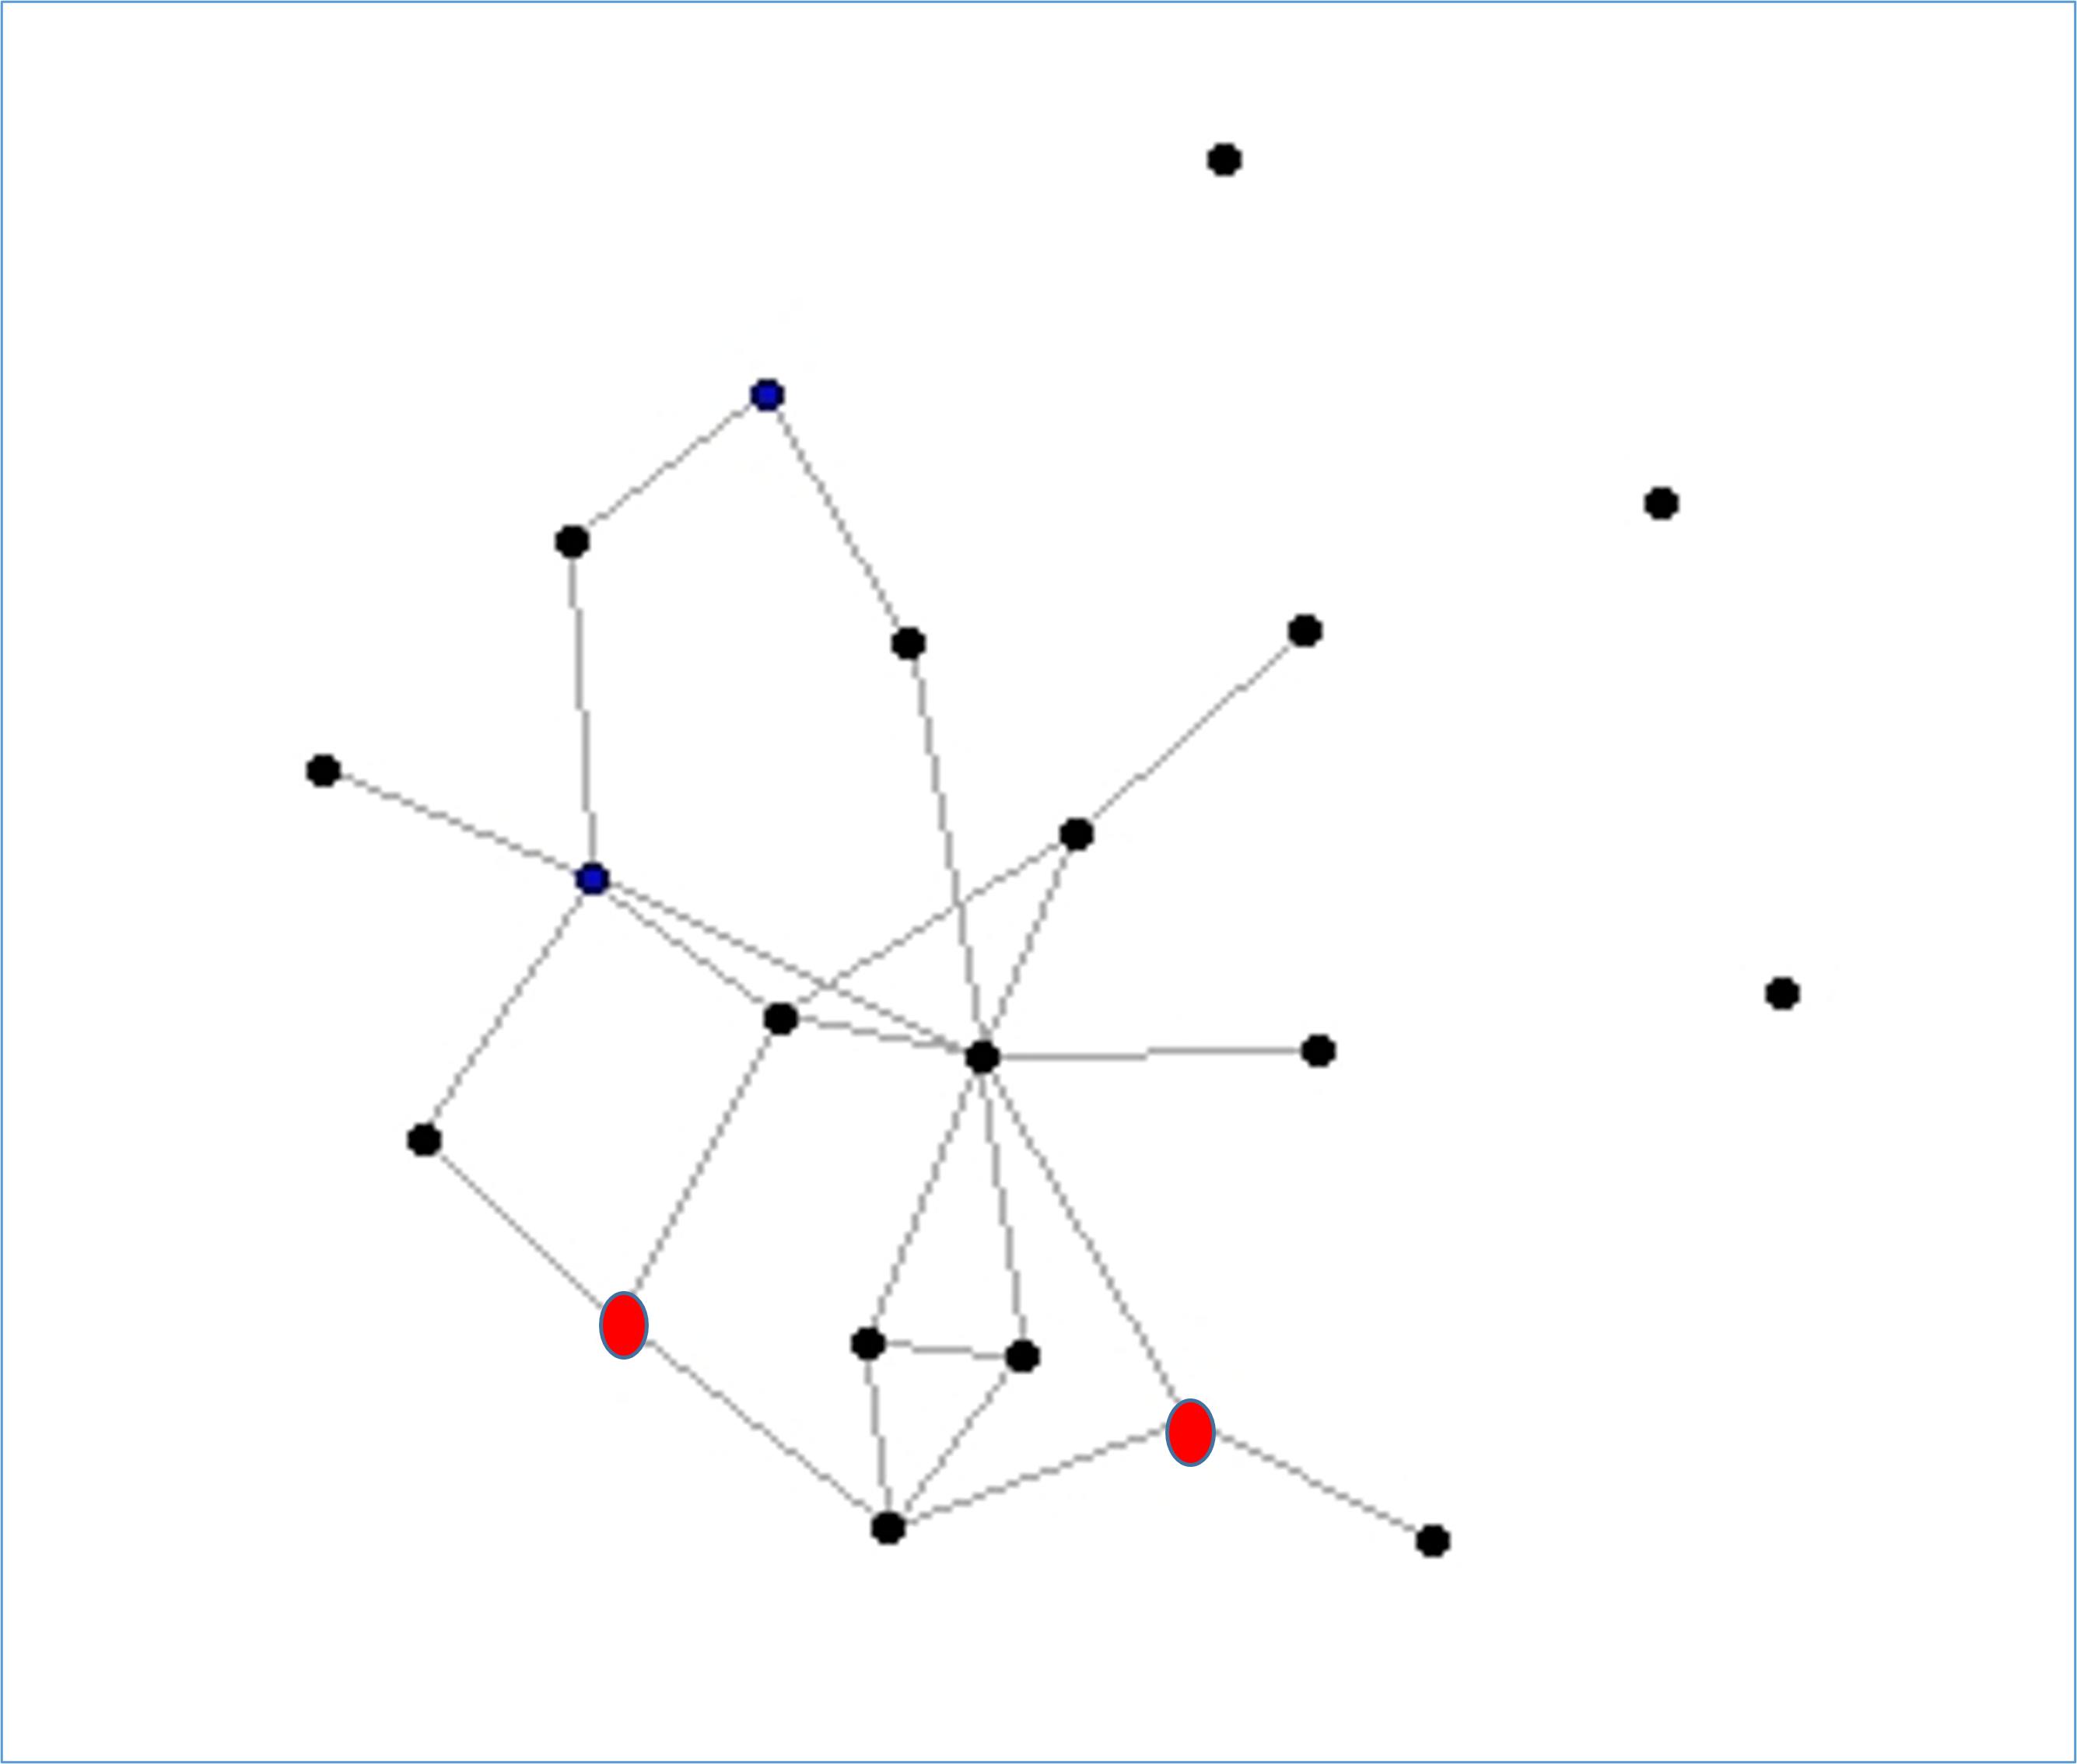
\includegraphics[scale=0.5]{Original Figures/Network Example 1.png}
    \caption{One possible realization of a simple network where $m = 2$ individuals are living with HIV (red nodes), and $N=R-m = 18$ individuals are currently uninfected (black nodes).}
    \label{fig: Figure 2}
\end{figure}

Suppose that the network links represent sexual partnerships. We can see from Figure \ref{fig: Figure 2} that only subset of individuals, $n$, have sexual partners living with HIV/AIDS at baseline (in this realization of the network, $n=5$ direct partnership contacts). For these $n$ individuals, their risk of acquiring HIV will be some probability $p$ between 0 and 1. On the other hand, the remaining $N-n$ uninfected individuals who have no sexual partners living with HIV/AIDS (here, 13 individuals) will have a probability of acquiring HIV equal to 0 (ignoring other transmission routes for simplicity). Thus, for each uninfected individual their probability of infection will be either $p_i$ or 0, while the average risk of infection in the population overall after one time step will be estimated by:
\begin{equation}\label{eq:9}
Y_{i}\left(\mathbf{\alpha} =0|G=g\right) = \frac{\sum_{i=1}^{n}(p_{i})}{N} = \frac{n\bar{p}}{N}.
\end{equation}

Now consider an intervention package delivered to this same population such that some proportion $k/N$ uninfected individuals receive PreP.  Following the intervention, the $n$ individuals who have a sexual partner living with HIV/AIDS will have either the same probability $p$ of infection as before or a lower probability $p'$ of infection if they are receiving PreP, since PreP aims to prevent infection following infectious exposure. 

Among the individuals with no partners living with HIV/AIDS, the risk of infection will remain unchanged at 0. If our intervention package happens to only deliver PreP to this latter group, the average risk of infection in the population will remain at $np/N$ regardless of the proportion of individuals given Prep. On the other hand, if we had distributed PreP only to individuals with infectious contacts, the average risk of infection would have been reduced. When $n=k$ and PreP is distributed to only those with infectious contacts, the average population risk is $kp'/N$.

Why does this matter? Our goal is to estimate how the HIV infection risk changes when we do versus do not deliver the intervention package to this network. But we can see from the above that the intervention “give PreP to $n$ individuals” can be implemented in a range of ways, resulting in a range of possible counterfactual outcomes for infection under the intervention package even when the network is the same. In general, we would expect this effect to be bounded between 0 and $(kp'/N - kp/N)$ for any single network structure, and the overall effect will then depend on the distribution of possible network structures. 

As an example, consider Figure \ref{fig: Figure 3}  below. In this image, a random 10\% of uninfected individuals have been assigned to receive PreP. In this particular realization of the network intervention, it happens that all individuals assigned to PreP are in fact not exposed. For those individuals, PreP does not change their initial probability of HIV infection; and for the entire network, the addition of PreP does not change the expected incidence of infection over the next time step.
\begin{figure}[H]
    \centering
    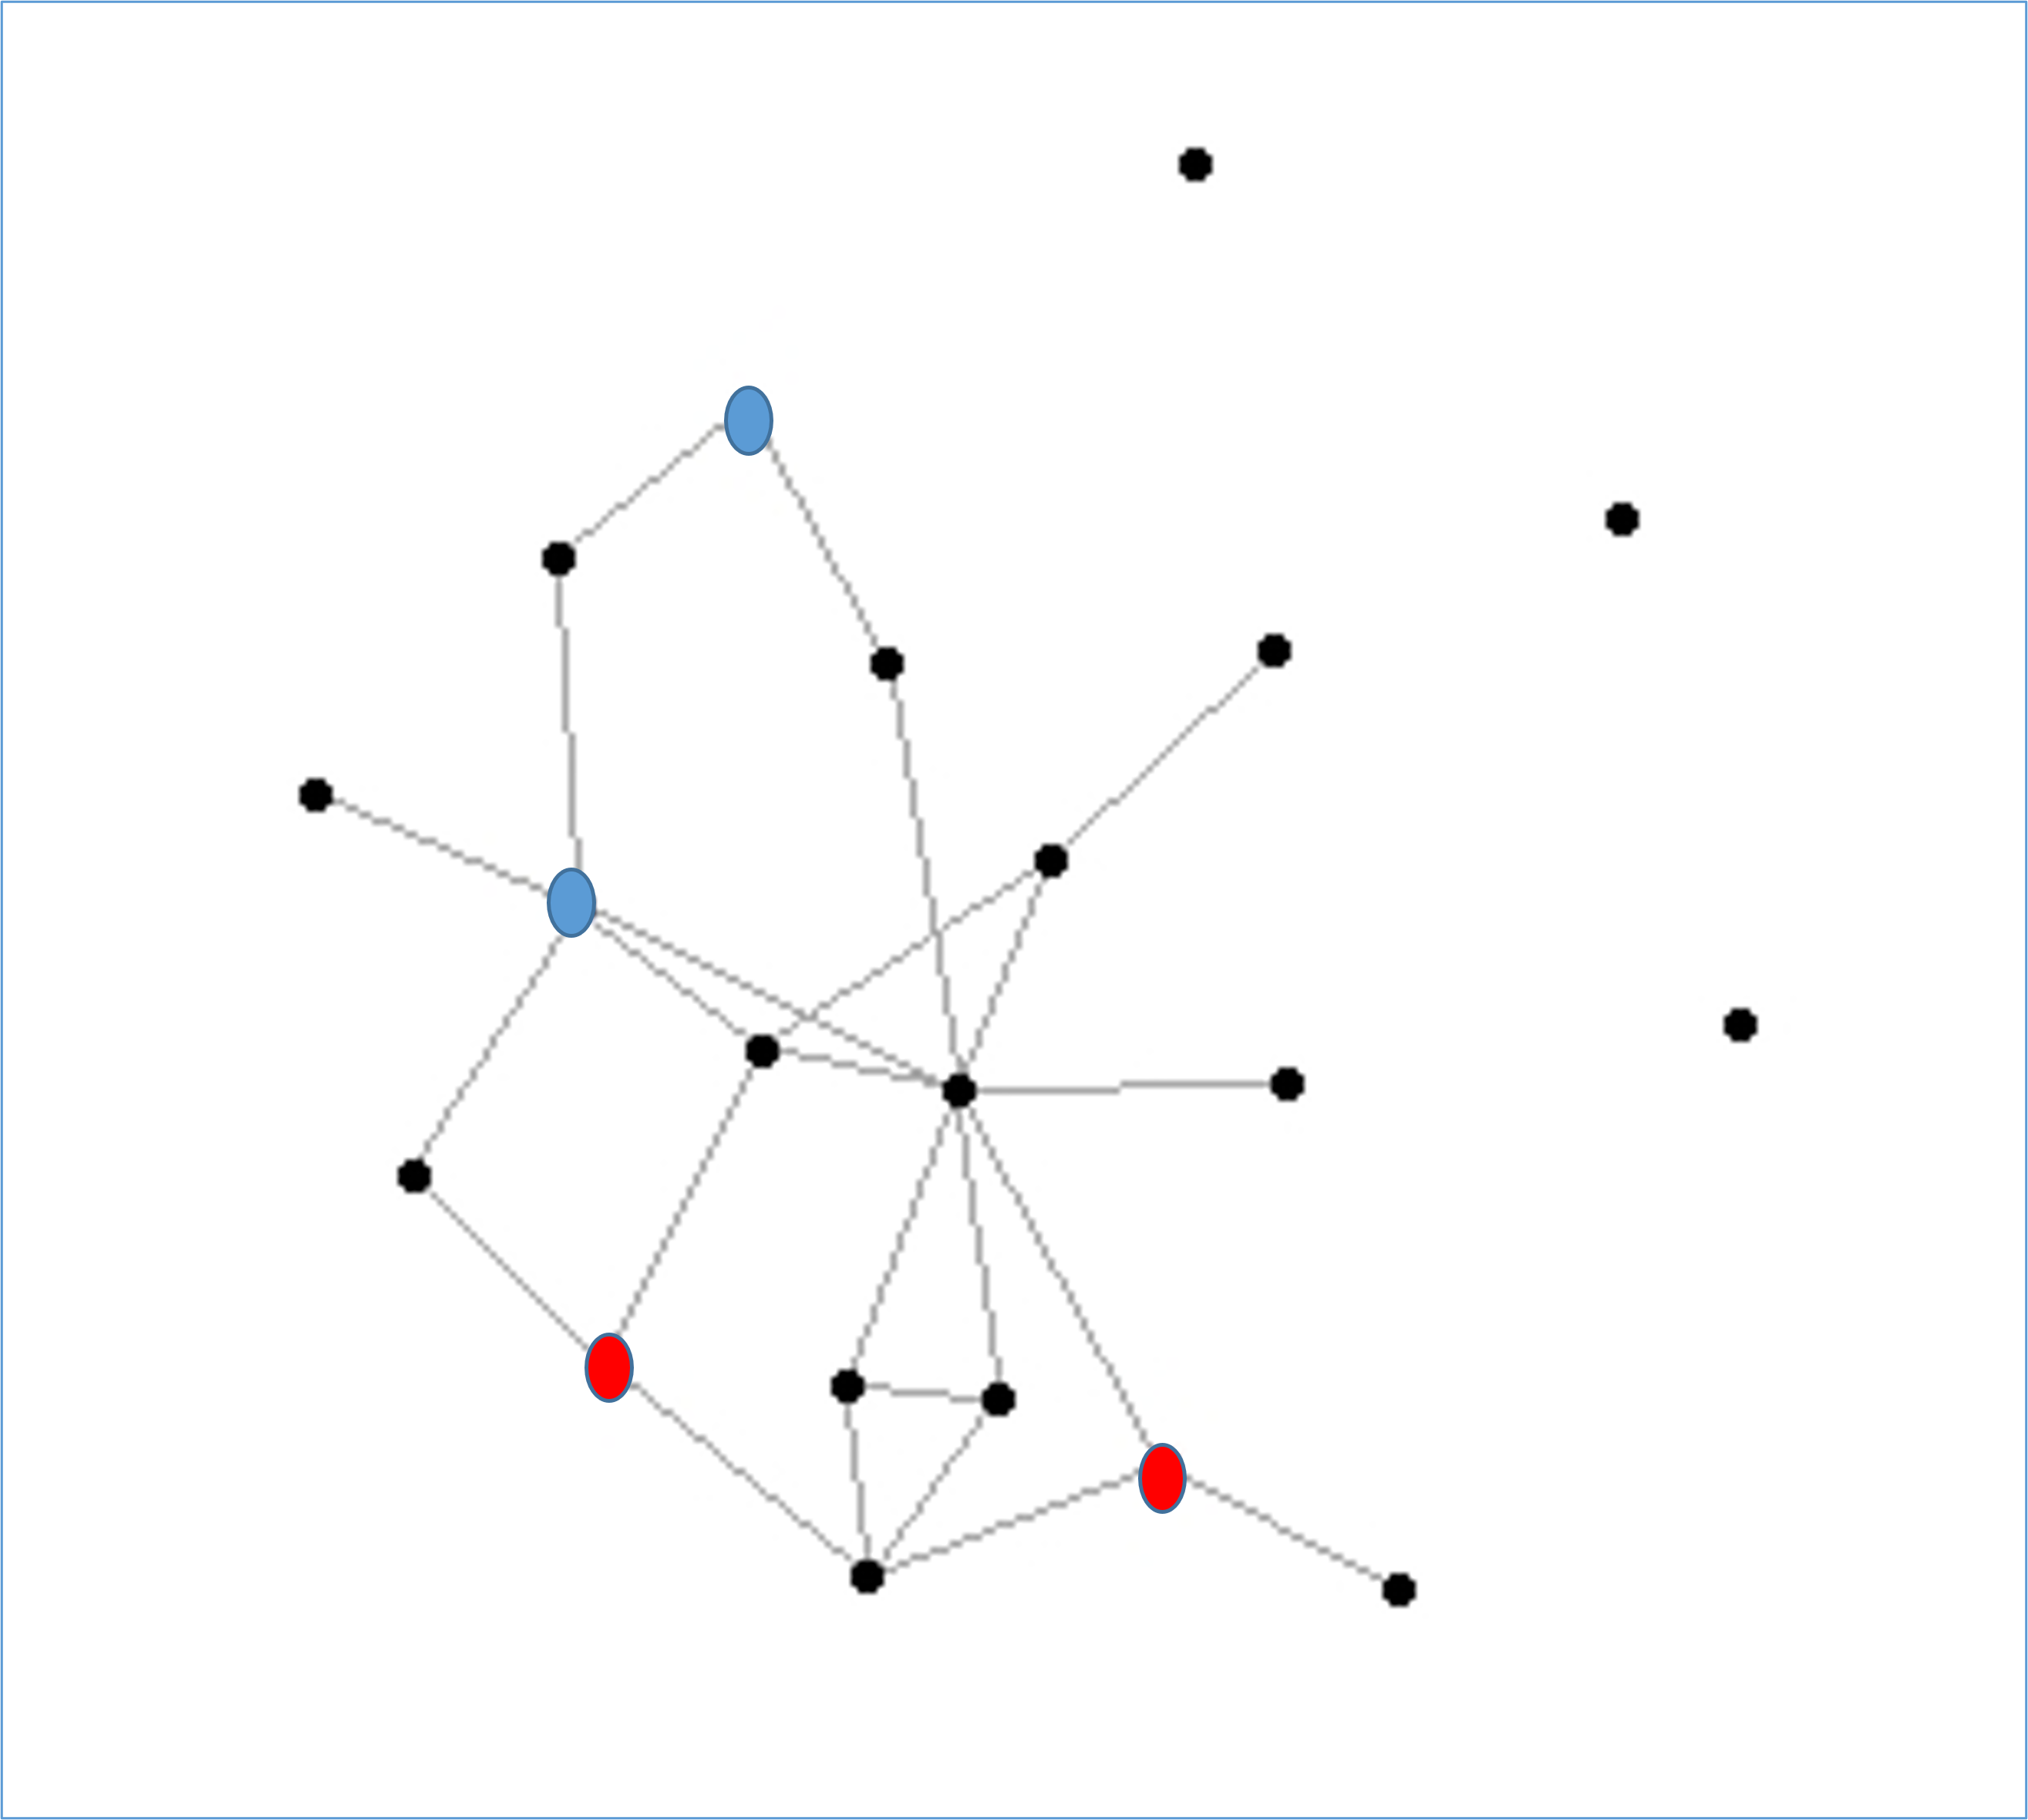
\includegraphics[scale=0.5]{Original Figures/Network Example 2.png}
    \caption{Random PrEP assignment to the network with 10\% coverage of uninfected individuals. The 2 blue nodes represent uninfected individuals assigned to PrEP; red nodes represent individuals living with HIV; black nodes are individuals without HIV and not assigned to PreP.}
    \label{fig: Figure 3}
\end{figure}

After PrEP assignment in Figure \ref{fig: Figure 3}, the counterfactual outcome over the next time step can be estimated using Equation \ref{eq:9} as follows:

\begin{align}
\begin{split}
Y_{i}\left(\mathbf{\alpha}|G=g\right) & = \frac{\sum_{i=1}^{n}(p_{i})}{N}  \\ 
& = P\left(Y|PrEP = 0, Contact = 1\right)P\left(PrEP = 1, Contact = 1\right)  \\ \nonumber
& +P\left(Y|PrEP = 0, Contact = 0\right)P\left(PrEP = 1, Contact = 0\right)  \\ \nonumber
& +P\left(Y|PrEP = 1, Contact = 1\right)P\left(PrEP = 0, Contact = 1\right) \\ \nonumber
&  +P\left(Y|PrEP = 1, Contact = 0\right)P\left(PrEP = 0, Contact = 0\right) \\ \nonumber
 &=  \frac{5}{18}*p_1 +  \frac{11}{18}*0 +\frac{0}{18}*p_2 +  \frac{2}{18}*0 \\ \nonumber
 &=\frac{5p_1}{18}  \nonumber
\end{split}
\end{align}

No individuals have both PrEP and an infectious contact, so the value of $p_2$ does not matter in this particular realization. Likewise, for individuals who have no infectious contacts, regardless of PrEP status they have no probability of infection (in the first time step). Therefore, the outcome will be entirely driven by the probability of transmission with an infectious contact and no PrEP, $p_1$.

Now, assume we are interested in estimating the causal effect of increasing PrEP coverage in networks of this type. A common network simulation approach would be to generate a new network with the same properties as the original network, but in which the PrEP coverage is more common -- say 20\%. Figure \ref{fig:Figure 6} gives an example using a new randomly generated network.

\begin{figure}[H]
    \centering
    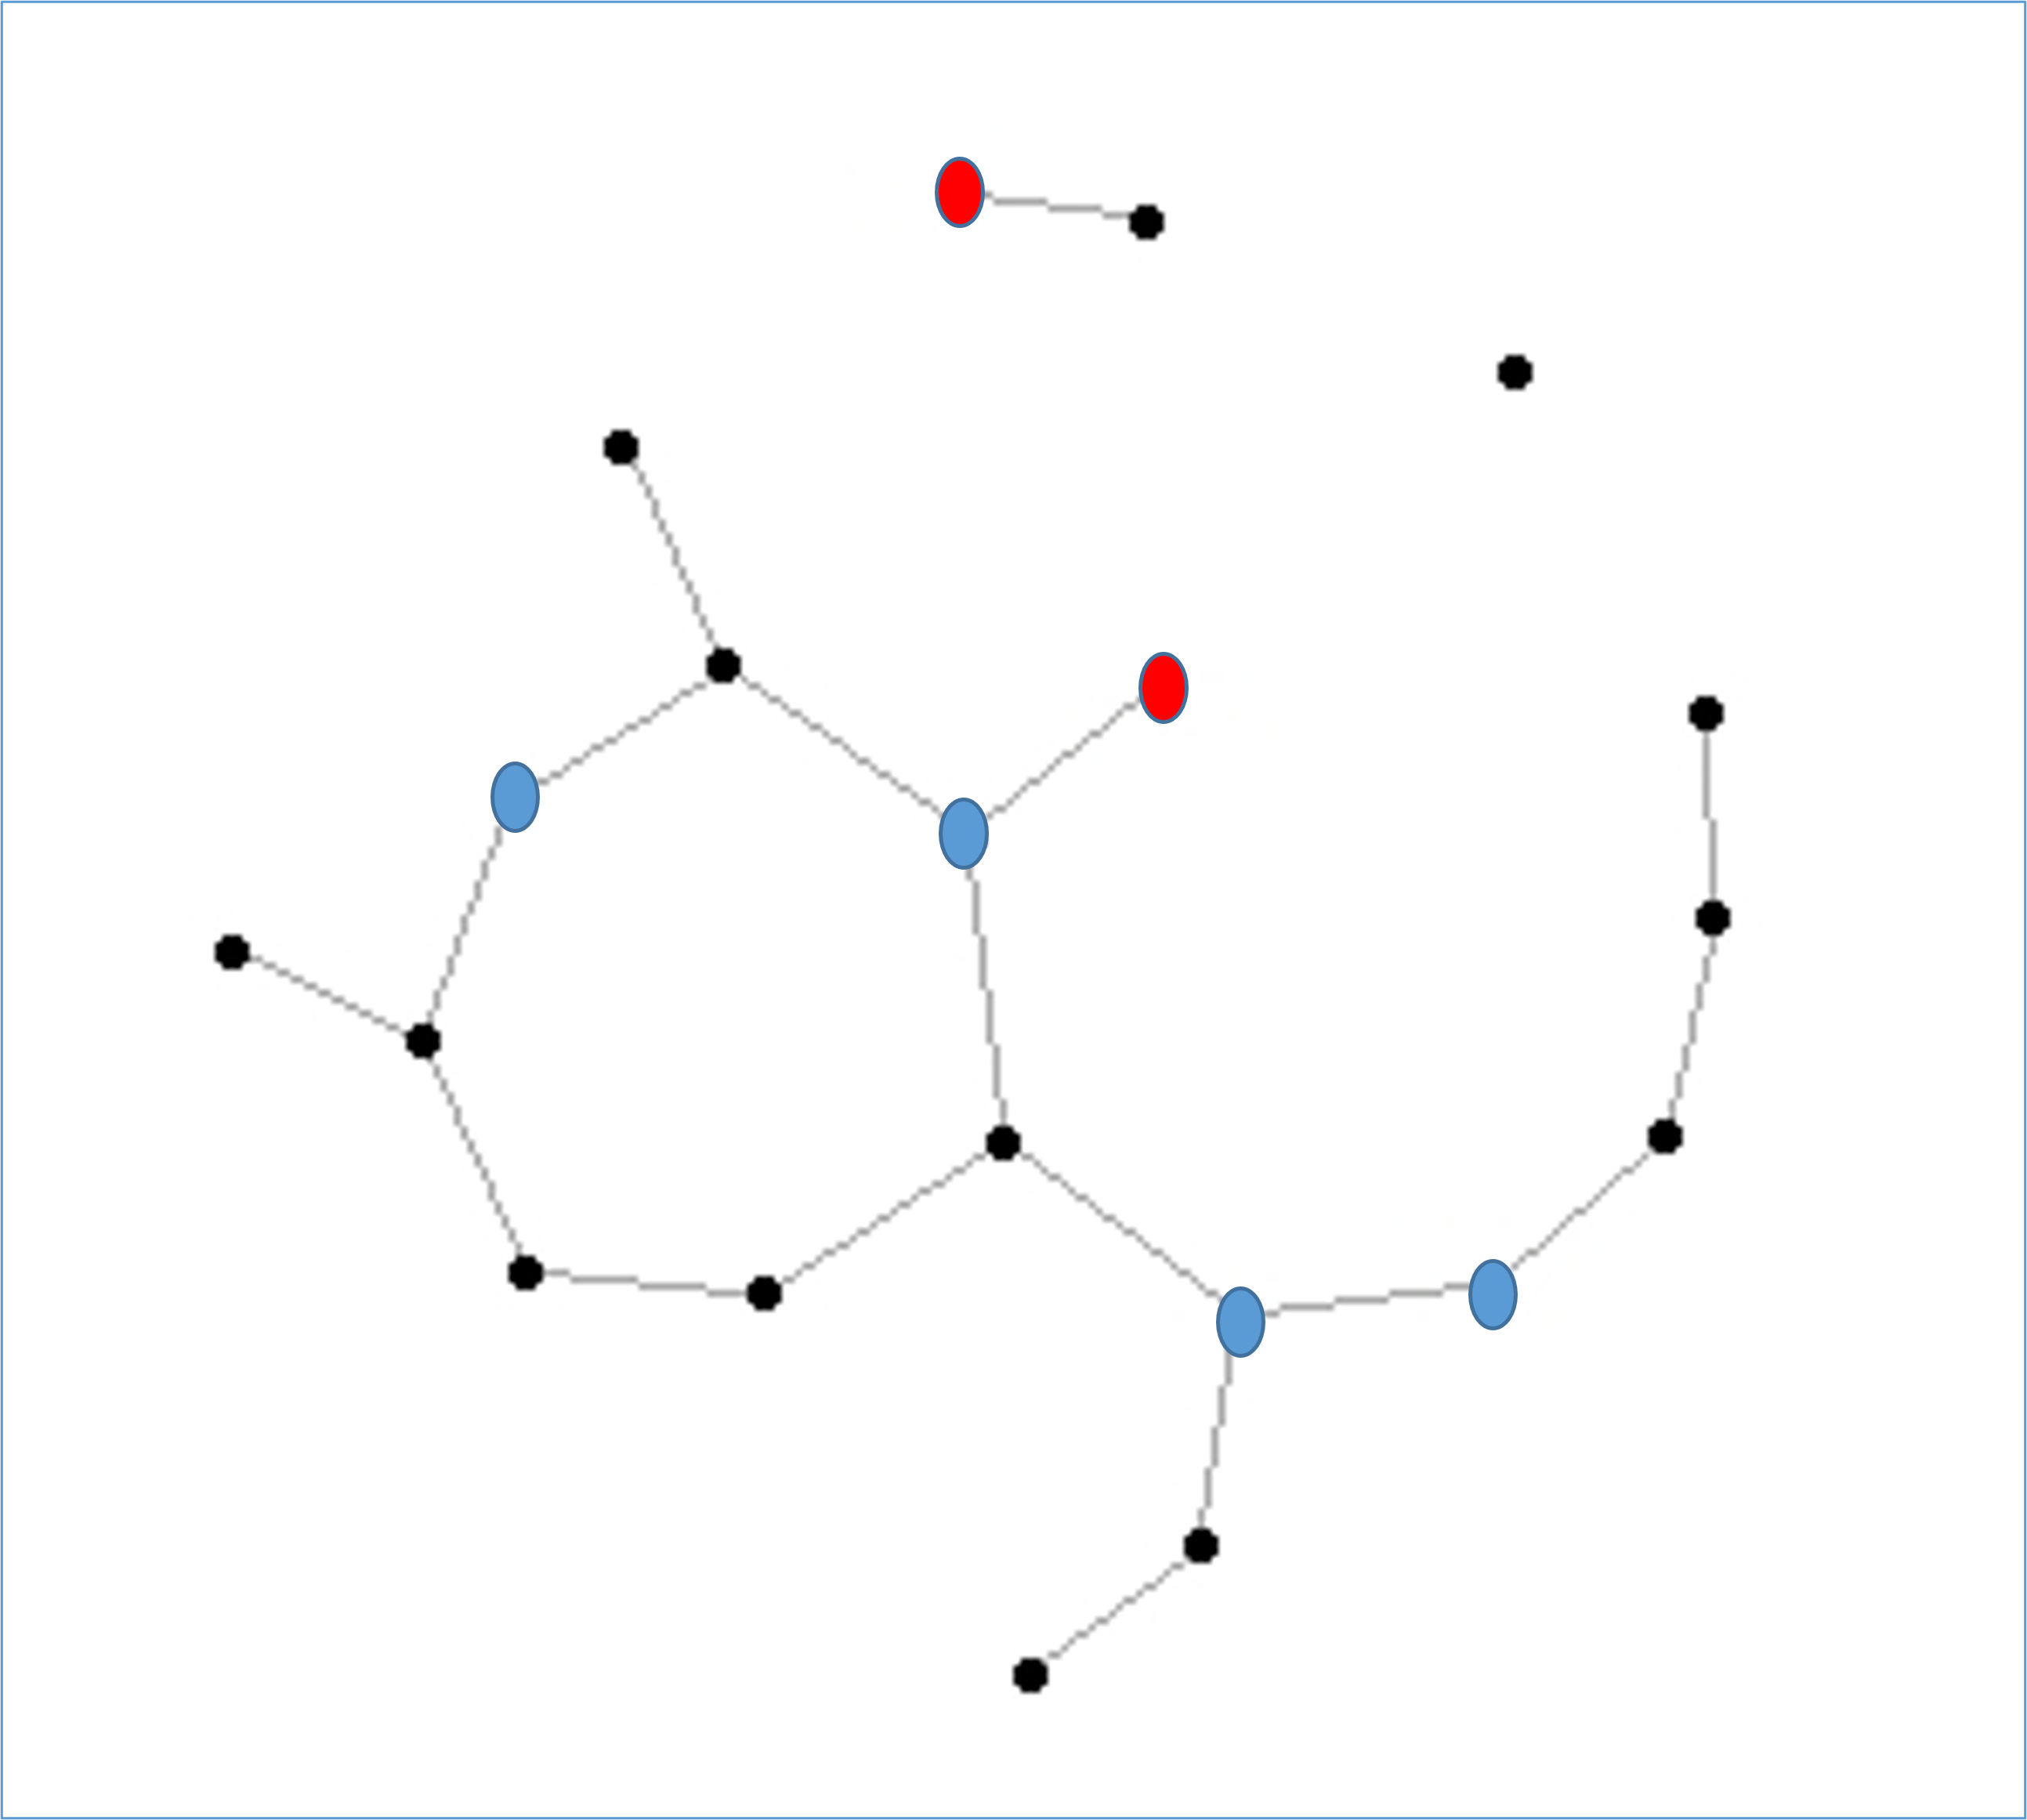
\includegraphics[scale=0.5]{Original Figures/Network Example 5.png}
    \caption{Re-generated network with 20 \% PrEP coverage randomly assigned to uninfected individuals. The 4 blue nodes represent uninfected individuals assigned to PrEP; the 2 red nodes represent individuals living with HIV; the 14 black nodes are individuals without HIV and not assigned to PrEP. }
    \label{fig:Figure 6}
\end{figure}

We can immediately see from comparison with the previous two figures that the structure of this new network is different. However, it still follows the same basic network parameters as the previous network. With the same number of individuals, same baseline HIV prevalence, and same probability of network contacts. There are once again 2 individuals living with HIV and 18 uninfected individuals. Now, 4 uninfected individuals have been assigned to PrEP, only one of whom has an infectious contact. In addition, one other individual not assigned to PrEP has an infectious contact; the remaining 14 uninfected individuals do not have infectious contacts. Now, the counterfactual outcome estimated using Equation \ref{eq:9} will depend on the probability of transmission following an infectious contact while on PrEP and while not on PrEP:

\begin{align}
\begin{split}
Y_{i}\left(\mathbf{\alpha*}|G=g*\right) & = \frac{\sum_{i=1}^{n}(p_{i})}{N}  \\ 
& = P\left(Y|PrEP = 0, Contact = 1\right)P\left(PrEP = 1, Contact = 1\right)  \\ \nonumber
& +P\left(Y|PrEP = 0, Contact = 0\right)P\left(PrEP = 1, Contact = 0\right)  \\ \nonumber
& +P\left(Y|PrEP = 1, Contact = 1\right)P\left(PrEP = 0, Contact = 1\right) \\ \nonumber
&  +P\left(Y|PrEP = 1, Contact = 0\right)P\left(PrEP = 0, Contact = 0\right) \\ \nonumber
 &= \frac{1}{18}*p_1 +  \frac{14}{18}*0 +\frac{1}{18}*p_2 +  \frac{3}{18}*0 \\ \nonumber
 &=\frac{p_1+p_2}{18}  \nonumber
 \end{split}
\end{align}

If we were to use this network to estimate the causal effect, without taking the fact that these are network-specific counterfactuals into consideration, we might conclude that this estimates the effect of increasing PrEP coverage from 10\% to 20\% . However, when we consider the quantities that were actually estimated on each network, we notice that this does not estimate either a network-specific effect nor an average effect across possible networks unless we can assume that network structure does not affect the counterfactual outcome. 

\begin{equation}\label{eq:12}
Y_{i}\left(\mathbf{\alpha*}|G=g*\right) -Y_{i}\left(\mathbf{\alpha}|G=g\right) = \frac{\left(p_1 +p_2\right)-\left(5p_1\right)}{18}= \frac{p_2-4p_1}{18}.
\end{equation}


Next consider a scenario where we retain the original network structure from Figure \ref{fig: Figure 2}, but apply additional PrEP assignment. There are multiple ways in which we can do this, but for simplicity we consider the following two options. In the first, we increase PrEP coverage to 20\% by selecting an additional random 10\% of uninfected individuals to receive treatment (Figure \ref{fig: Figure 4}). In the second, we discard prior treatment status and choose a random 20\% to receive PrEP (Figure \ref{fig:Figure 5}).


\begin{figure}[H]
    \centering
    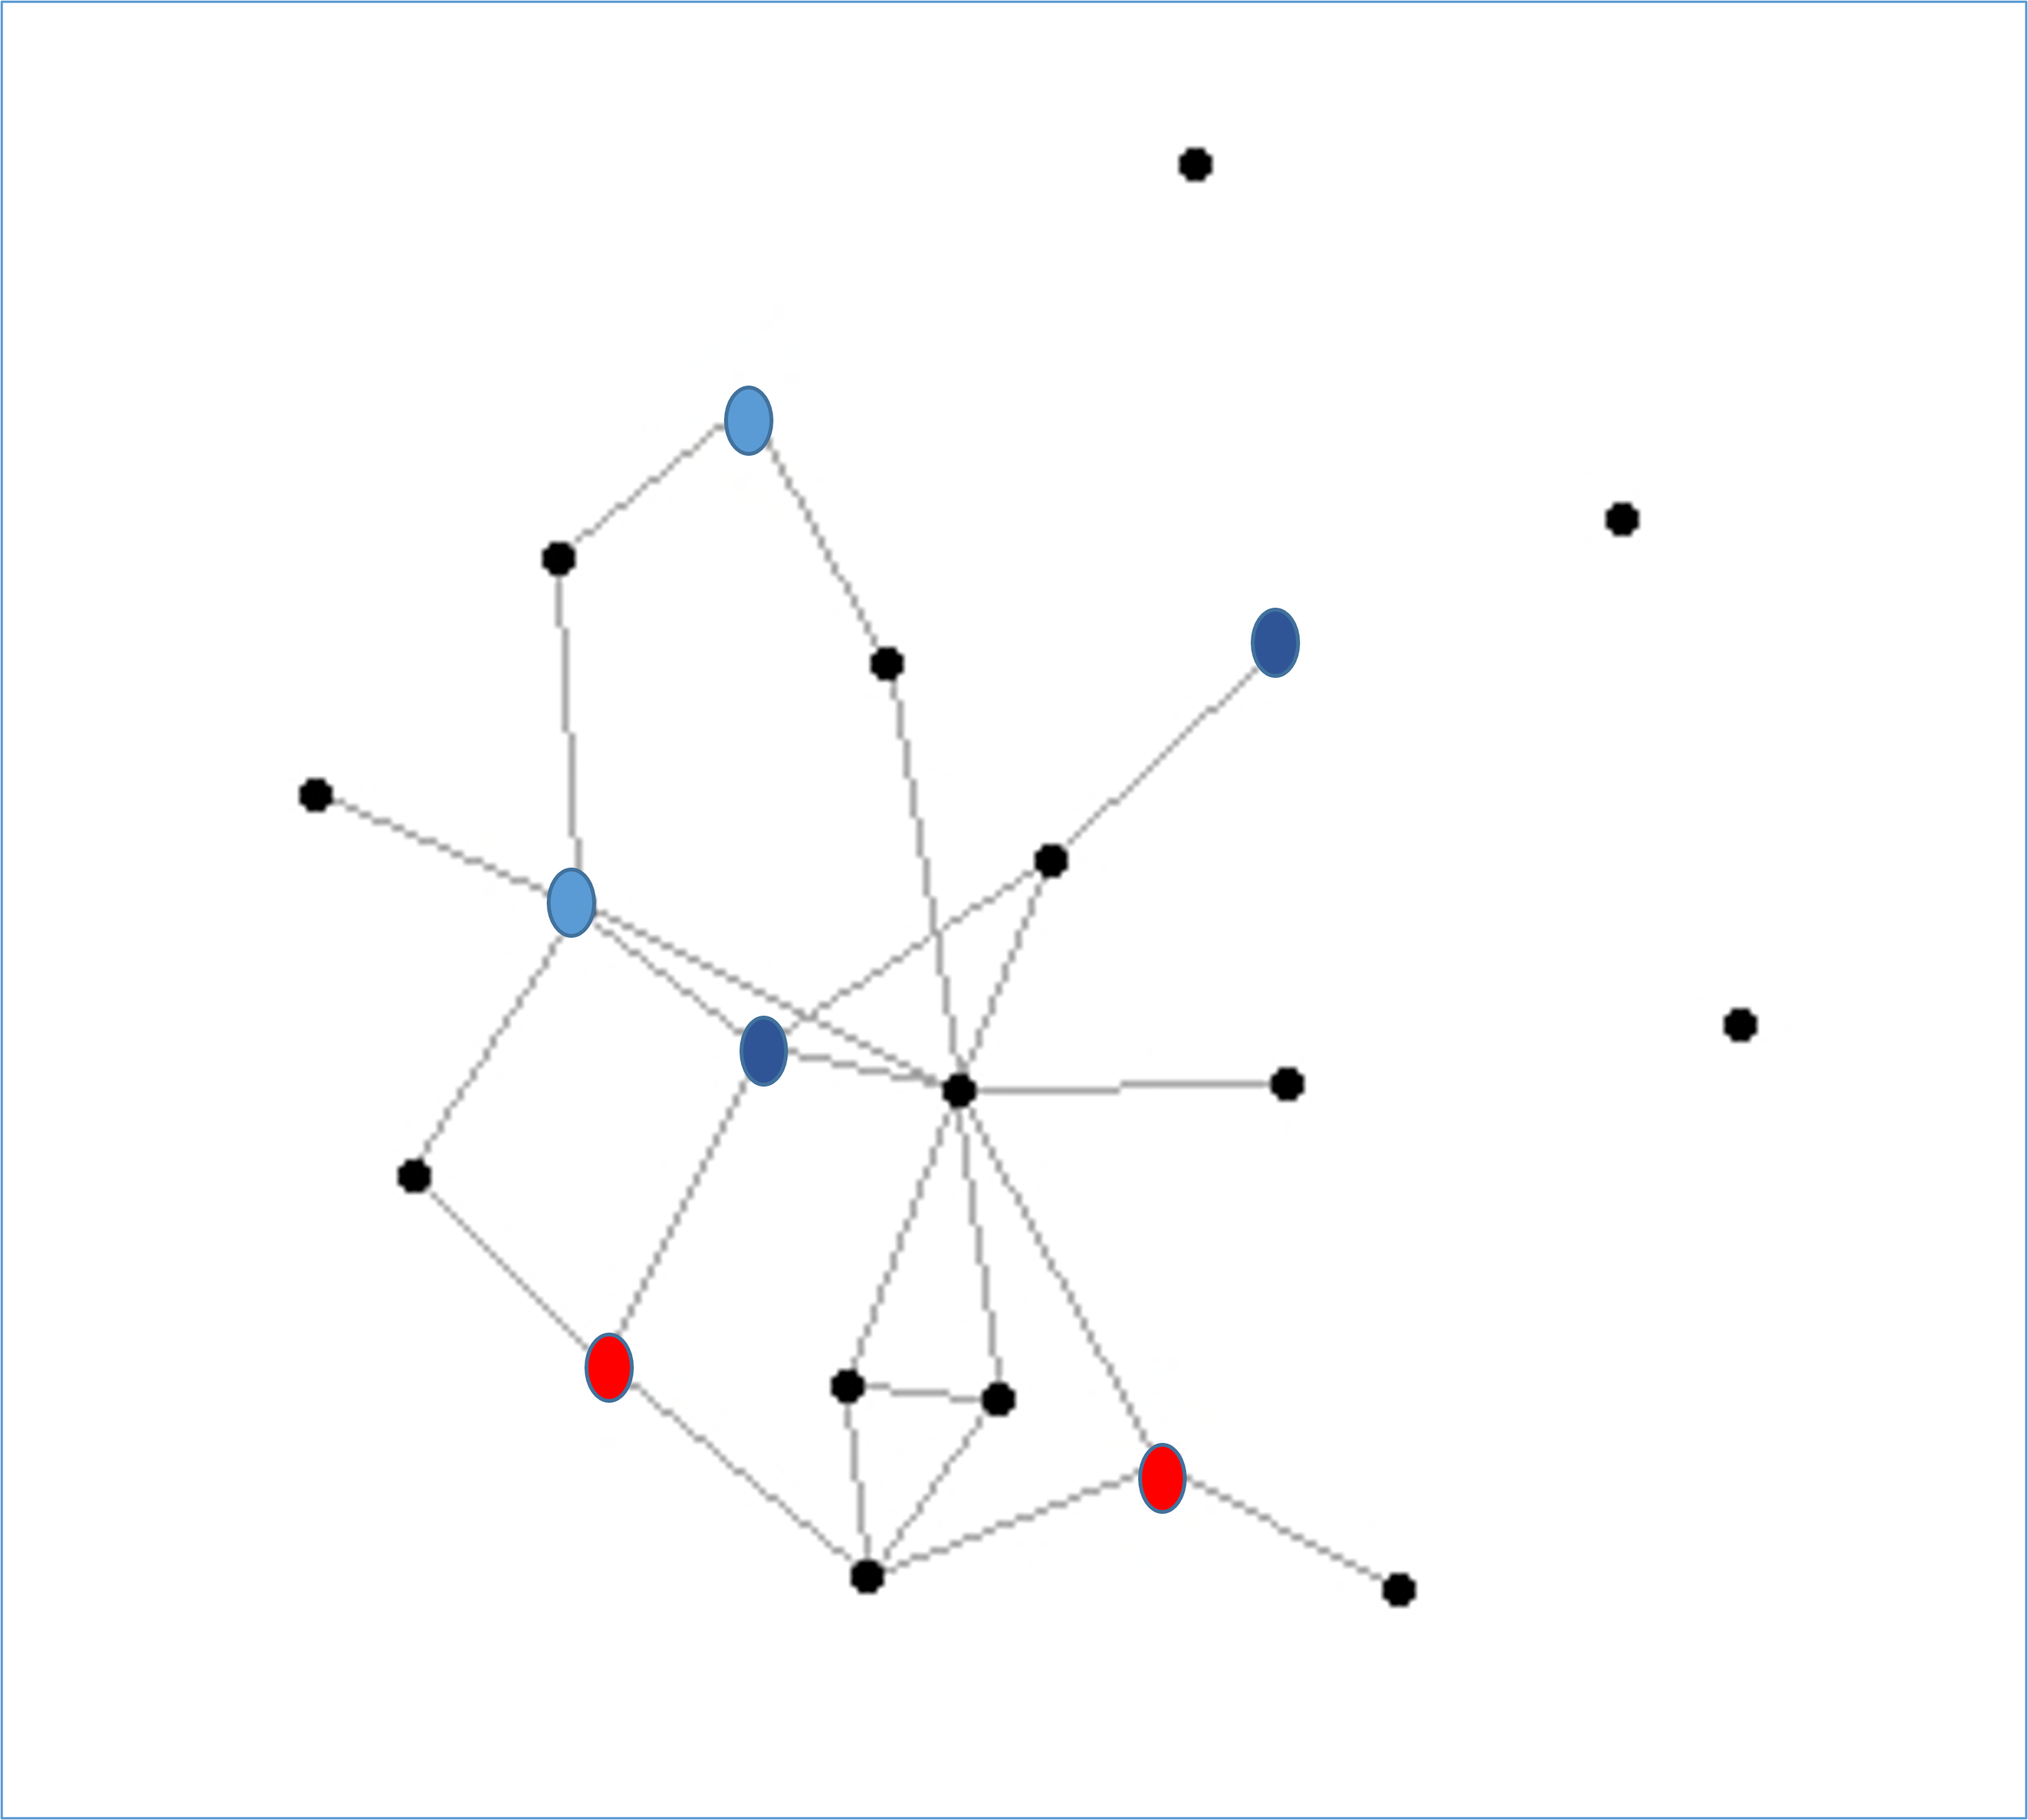
\includegraphics[scale=0.5]{Original Figures/Network Example 4.png}
    \caption{Additive scenario: Network structure from the control scenario, with an additional 10\%  of uninfected individuals randomly assigned to PreP. Blue nodes represent uninfected individuals assigned to PrEP; red nodes represent individuals living with HIV; black nodes are individuals without HIV and not assigned to PrEP.}
    \label{fig: Figure 4}
\end{figure}

Under the Additive treatment pattern, the original two individuals who were treated but did not have infectious contacts continue to receive treatment. We now additionally provide PrEP to two more randomly selected individuals, of whom one dose have an infectious contact. Of the remaining 14 uninfected and untreated individuals, 4 have infectious contacts. We now obtain the following estimate: 

\begin{align}
\begin{split}
Y_{i}\left(\mathbf{\alpha*}|G=g\right) & = \frac{\sum_{i=1}^{n}(p_{i})}{N}  \\ 
& = P\left(Y|PrEP = 0, Contact = 1\right)P\left(PrEP = 1, Contact = 1\right)  \\ \nonumber
& +P\left(Y|PrEP = 0, Contact = 0\right)P\left(PrEP = 1, Contact = 0\right)  \\ \nonumber
& +P\left(Y|PrEP = 1, Contact = 1\right)P\left(PrEP = 0, Contact = 1\right) \\ \nonumber
&  +P\left(Y|PrEP = 1, Contact = 0\right)P\left(PrEP = 0, Contact = 0\right)\\ \nonumber
 &= \frac{4}{18}*p_1 +  \frac{10}{18}*0 +\frac{1}{18}*p_2 +  \frac{3}{18}*0\\ \nonumber
 &=\frac{4p_1+p_2}{18}  \nonumber
 \end{split}
\end{align}

\begin{figure}[H]
    \centering
    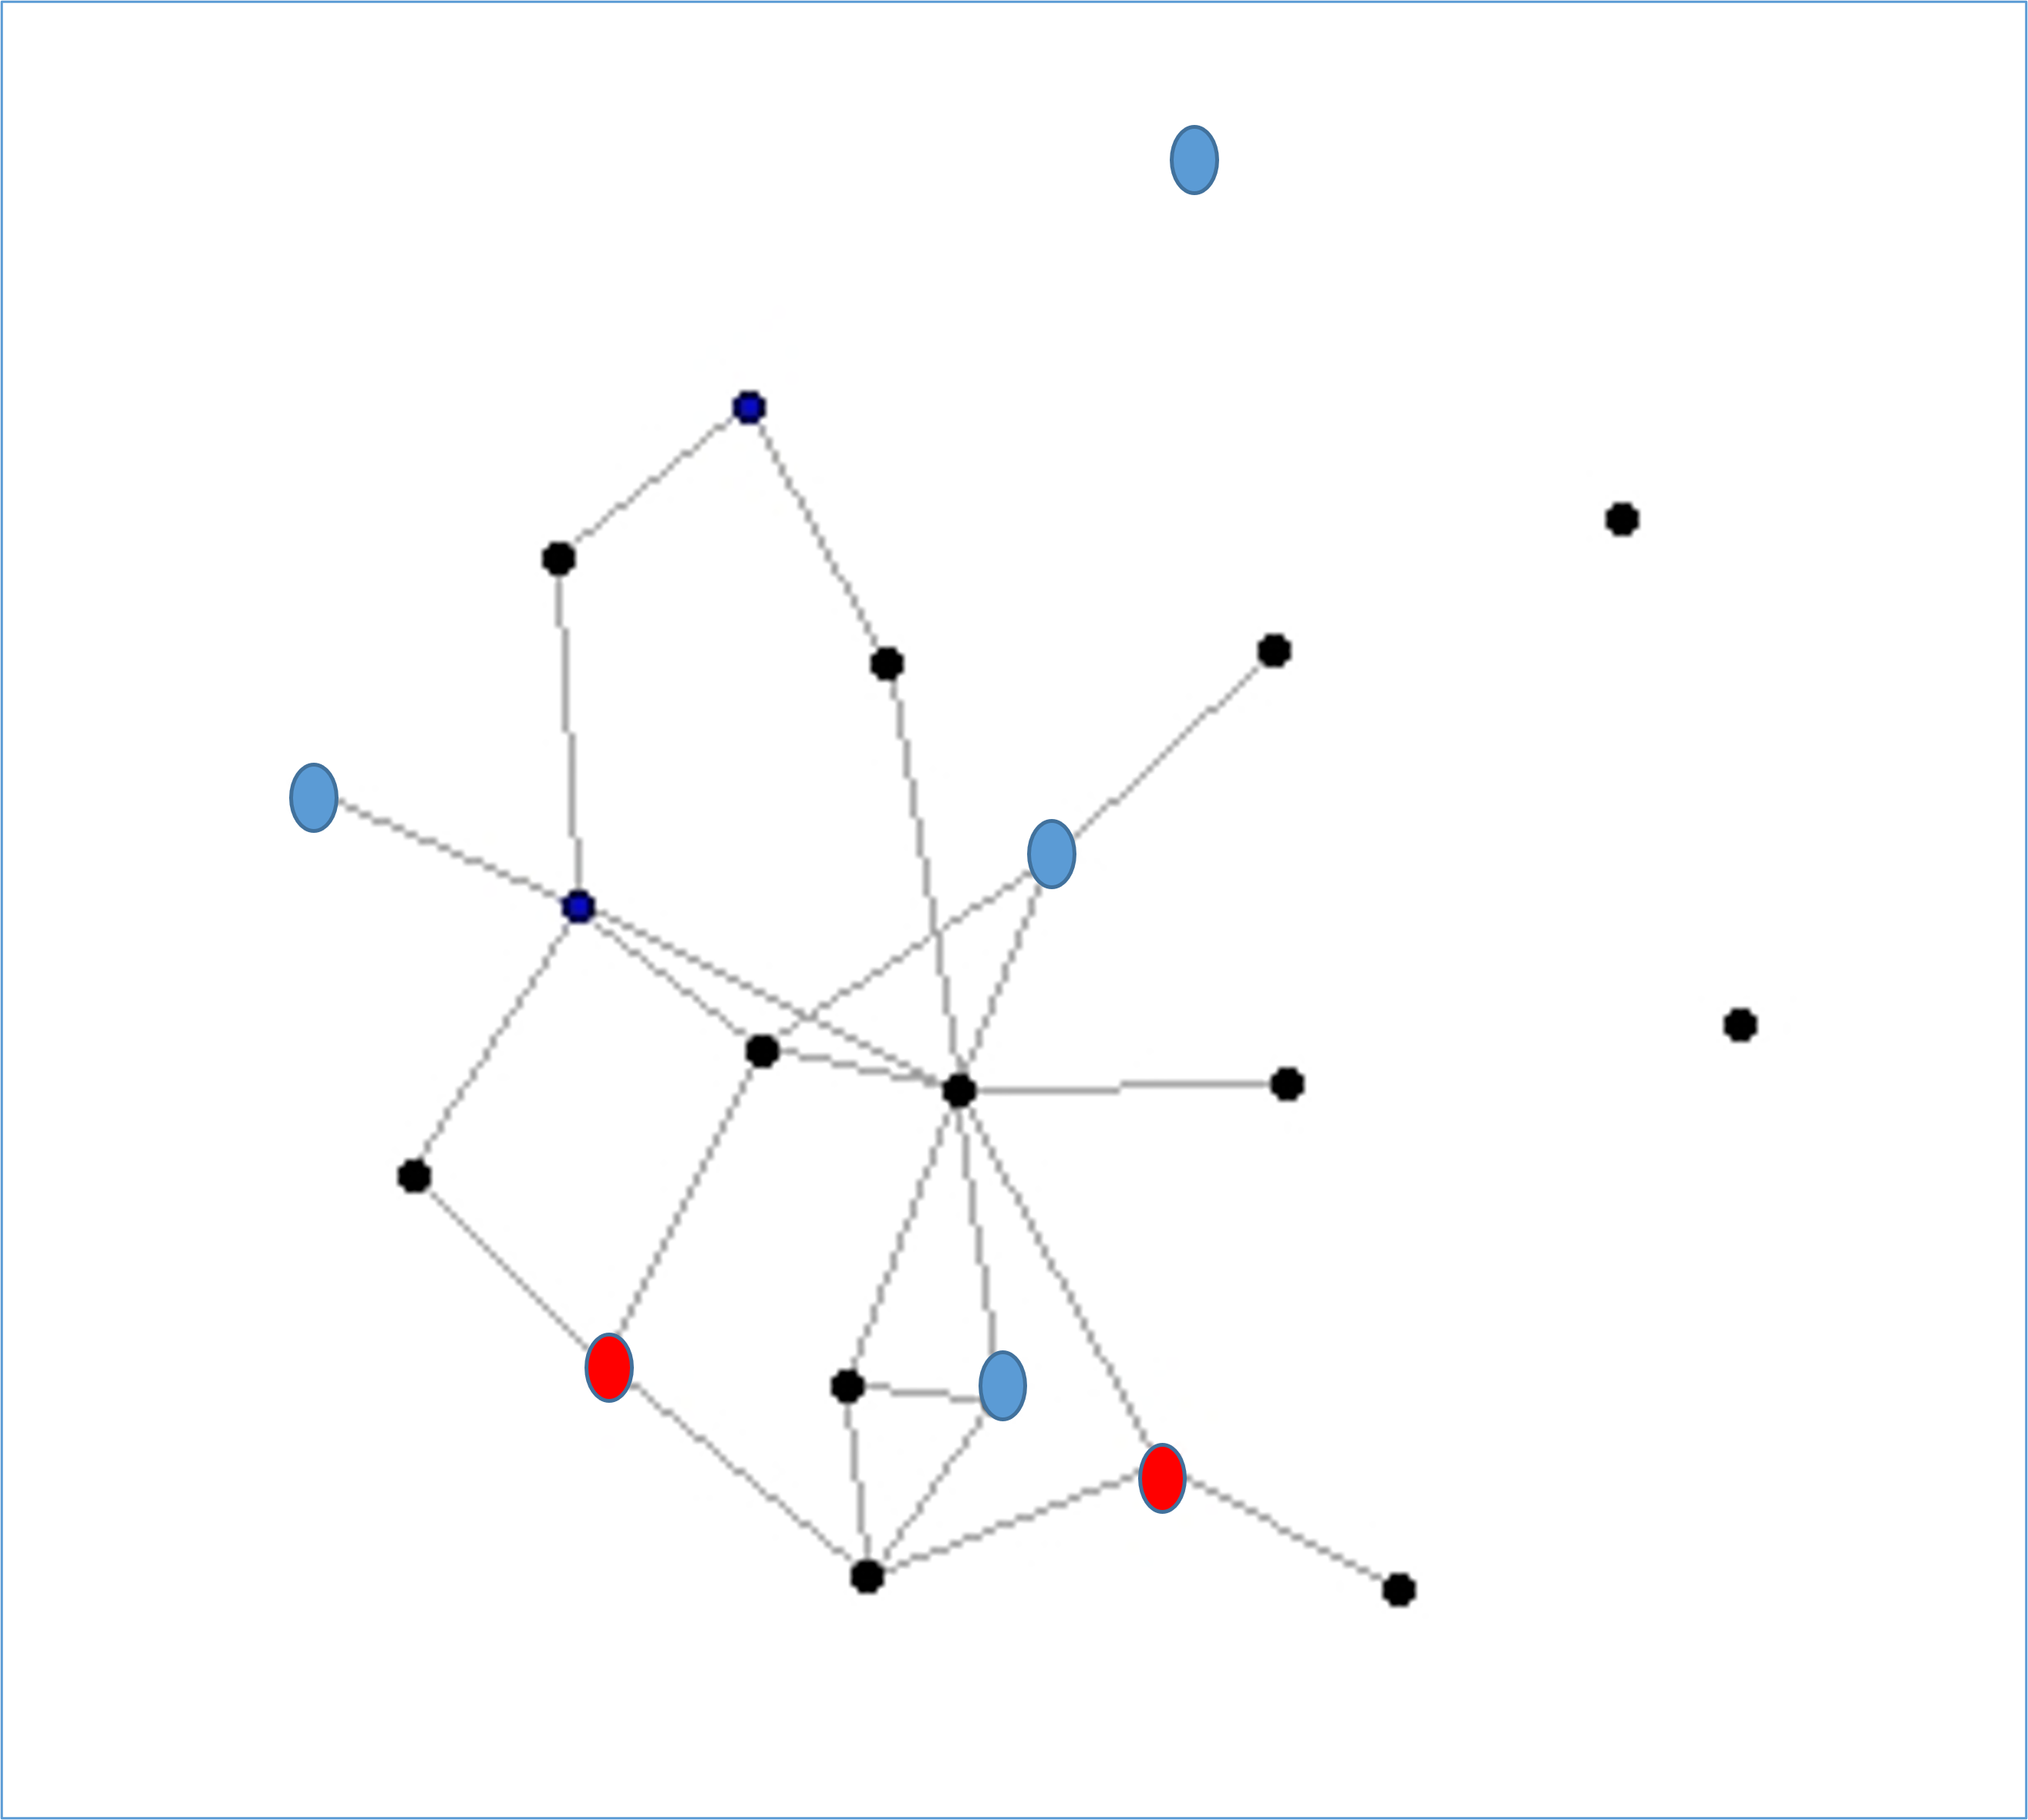
\includegraphics[scale=0.5]{Original Figures/Network Example 3.png}
    \caption{Random scenario: Network structure from the control scenario, with a newly selected 20\%  of uninfected individuals randomly assigned to PreP. Blue nodes represent uninfected individuals assigned to PrEP; red nodes represent individuals living with HIV; black nodes are individuals without HIV and not assigned to PreP.}
    \label{fig:Figure 5}
\end{figure}

Under the Random treatment pattern, all four of the newly selected PrEP recipients do not have an infectious contact. Of the remaining 14 uninfected and untreated individuals, 5 have infectious contacts. This time, we obtain the following estimate: 

\begin{align}\label{eq:14}
\begin{split}
Y_{i}\left(\mathbf{\alpha**}|G=g\right) & = \frac{\sum_{i=1}^{n}(p_{i})}{N}  \\ 
& = P\left(Y|PrEP = 0, Contact = 1\right)P\left(PrEP = 1, Contact = 1\right)  \\ \nonumber
& +P\left(Y|PrEP = 0, Contact = 0\right)P\left(PrEP = 1, Contact = 0\right)  \\ \nonumber
& +P\left(Y|PrEP = 1, Contact = 1\right)P\left(PrEP = 0, Contact = 1\right) \\ \nonumber
&  +P\left(Y|PrEP = 1, Contact = 0\right)P\left(PrEP = 0, Contact = 0\right)\\ \nonumber
 &= \frac{5}{18}*p_1 +  \frac{10}{18}*0+\frac{0}{18}*p_2 +  \frac{4}{18}*0  \\ \nonumber
 &=\frac{5p_1}{18}  \nonumber
 \end{split}
\end{align}

Comparing these results to our initial 10\% PrEP coverage scenario, we obtain the following estimates. For the Additive treatment pattern, we get:

\begin{equation}\label{eq:15}
E\left[Y_{i}\left(\mathbf{\alpha*}-\mathbf{\alpha}|G=g\right)\right] =  Y_{i}\left(\mathbf{\alpha*}|G=g\right) -Y_{i}\left(\mathbf{\alpha}= 0|G=g\right) = 
= \frac{\left(4p_1+p_2\right)-\left(5p_1\right)}{18}=
\frac{p2-p1}{18}
\end{equation}

and for the Random treatment pattern, we get:
\begin{equation}\label{eq:16}
E\left[Y_{i}\left(\mathbf{\alpha**}-\mathbf{\alpha}|G=g\right)\right] =Y_{i}\left(\mathbf{\alpha**}|G=g\right) -Y_{i}\left(\mathbf{\alpha}|G=g\right) = \frac{5p_1}{18} - \frac{5p_1}{18} =0.
\end{equation}

Note that like with the Regenerated network, all quantities in these contrasts are network-specific counterfactuals. However, unlike with the regenerated network, the new 20\% treatment counterfactuals are estimated conditional on the same network as the reference scenario counterfactuals. This provides a valid estimate of network-specific effects, even if these effects are not generalizable to all possible networks of this type. Also note that causal effects estimated by \ref{eq:15} and \ref{eq:16} are different, because they involve different treatment pattern comparisons.


\section{Amount of bias depends on network features}
In the previous section, we compared only two counterfactual estimates. More realistically, counterfactuals would be simulated multiple times each, so that the average effect could be estimated rather than the network-specific effect. As we have shown, the network-specific effect should be estimated by comparing network-specific counterfactuals before pooling across network realizations. However, this is only true because we cannot typically simulate all possible network realizations. We might expect then that as the number of realizations simulated increases to infinity, the potential bias from using the regeneration approach should reduce to zero.

Another important determinant of the expected bias is the size of the two parameters $n$ (individuals with infectious contacts) and $k$ (individuals receiving PrEP) relative to the size of the uninfected population $N$. If we randomly generate networks from our distribution, and randomly assign treatment to uninfected individuals, there are $\binom{N}{k}$ unique network realizations where $k$ individuals are treated. 

In each realization, some portion $n \le N$ will have an infectious contact. We can separate all possible network realizations into those in which at least one individual is both treated and has an infectious contact, and those in which all treated individuals have no infectious contact. Only for network realizations of the first type will treatment have any effect on the outcome -- when all treated individuals have no infectious contacts, there is no benefit to treatment. The proportion of networks where at least one treated individual has an infectious contact is (see Appendix \ref{Appendix 1} for derivation):

\begin{equation}\label{eq:17}
    \frac{{\binom{N}{k}}-{\binom{N-n}{k}}}{{\binom{N}{k}}}=1-\left(1-\frac{k}{N}\right)^{n}.
\end{equation}

That is, the probability of at least one node $i$ assigned to treatment with at least one infectious contact for a given network structure $g$ and treatment assignment is:
\begin{equation}\label{eq:18}
    P \coloneqq \mathbb{P}\left(n_{i}=1 \vert k_{i}=1,j,a,a*\right)=1-\left(1-\frac{k}{N}\right)^{n}.
\end{equation}
When $P$ is large, the majority of network realizations can be expected to contribute at least some information to the average effect. However, when $P$ is small, we can expect that most network realizations will be uninformative -- that is, most realizations of the network will be ones in which no individual is both treated and exposed to an infectious contact. Therefore, the magnitude of $P$ can provide insight into the number of realizations we need to simulate to obtain a stable estimate of effects across all network structures. In addition, note that
\begin{equation}\label{eq:19}
    \lim_{N \to \infty}P=\begin{cases}0 & k,n \text{ fixed} \\ 1 & k \to N \lor n \to N  \end{cases}
\end{equation}

That is, as the size of the uninfected network population increases, $P$ is expected to approach 0 for a fixed number of individuals receiving treatment and a fixed number with an infectious contact. On the other hand, if either the number of individuals treated or the number of individual with an infectious contact approaches the total number of uninfected individuals, then as $N$ increases, the value of $P$ will approach 1.

\section{Simulation example}
To demonstrate the potential impact of simulation approach, we repeated our simplified example across multiple network realizations. In the following section, we describe the simulation methods and results of this process.

\subsection{Methods}
We considered three types of network-based simulation models. Let $G=(V,E)$ be a graph representation of a network, with vertex set $V$ and edge set $E$. Let $N$ denote the \textit{order} of $G$, equal to the cardinality of the vertex set $\vert V \vert$. Network models were parameterized according to network size (graph order), and the generative model specifying the probability distribution from which the graph was drawn or the algorithm used to construct the graph. Let $deg(v)$ denote the degree of node $v$.

We first implemented the  Erdős–Rényi (ER) Random Graph Model with $G(N,p)$ parameterization, sclaing the edge formationn probability by the network size such that $p \coloneqq \frac{3}{N}$. This was done to avoid networks in which every susceptible individual had an infectious contact. 
% under which each of $N$ nodes has a binomially-distributed degree:
% \begin{equation*}
  %  \mathbb{P}(deg(v)=k)=\binom{n-1}{k}p^{k}\left(1-p\right)^{n-1-k}, \quad \forall v \in V . 
% \end{equation*}

We also implemented two other network generative models to assess the importance of specific aspects of network structure: \textit{preferential attachment} and \textit{clustering}. 

To assess preferential attachment we also implemented an Barabási–Albert (BA) scale-free graph model. This model involved constructing an initial connected graph, then adding a new nodes connected to the existing node $i$ with probability 
\begin{equation*}
    p_{i}=\frac{k_{i}}{\sum_{j}k_{j}}.
\end{equation*}

We use a generalization of the BA model, sometimes called the Nonlinear Preferential Attachment Model, with power parameter $\alpha$, where the degree distribution is given by:
\begin{equation*}
    p_{i}=\frac{k_{i}^{\alpha}}{\sum_{j}k_{j}^{\alpha}}.
\end{equation*}

Finally, to assess clustering, we used a Watts-Strogatz (WS) small world network model. The construction algorithm relied on 4 parameters: the dimension of the initial lattice (here always equal to 1), the size of the graph in each dimension (here always the final graph order $N$), the connected \textit{neighborhood size} $n$, and the rewiring probability $r$. The initial graph is a lattice where each node is connected to its $n$ neighbors. From the initial lattice graph, edges are randomly ``rewired", i.e. removed and connected to a different node, uniformly with probability $r$.

For each model type, we simulated the counterfactual infection probability after one time-step when 10\% of uninfected individuals were prescribed PrEP at random. We assume that treatment is assigned at random to all eligible (uninfected) individuals, with no attempt to target treatment based on an individual's outcome risk. While this is unrealistic for many real-world examples, in practice we generally do not with certainty whether an individual will or will not have an infectious contact at the time of treatment. In addition, we focus on a single time-step to avoid consideration of time-varying network structure changes.

In addition, we simulated comparison counterfactual data under 20\% of uninfected individuals prescribed PrEP, using the three approaches described in the previous simplified example: random reassignment of treatment on the same network realization (random condition); additive assignment of treatment on the same network realization (additive condition); and random reassignment of treatment on a regenerated network (regeneration condition). 

We estimated the average overall effect of 40\% versus 20\% PrEP coverage using the average counterfactual comparisons as described in the simplified example. Across a range of input parameters and model types, we present the risk difference estimate of the average overall effect using the following comparison approaches: (1) Additive approach -- 40\% coverage is achieved by adding an additional 20\% coverage to the existing 20\% coverage on a given network realization; (2) Random approach -- 40\% and 20\% coverage estimates obtained from random treatment on a given network realization; and (3) Regenerated approach -- 40\% and 20\% coverage estimates obtained from random treatment on different network realizations.

We varied the input parameters for each simulation model type as shown in the table below (Table \ref{tab:table1}).

\newpage
%%NOTE: please combine the two tables below with a column indicating which model type(s) the parameter applies to. Also, I'm not sure how to do the table caption, so please correct that. Thanks!
\begin{landscape}
\begin{table}[H]
    \centering
    \begin{tabular}{|c|c|c|c|c|}
    \hline
    \bf Parameter & \bf Model & \bf Alias in Code & \bf Default Value & \bf Range Considered  \\
    \hline
    Network size & Erdős–Rényi& $N$& 20 & $\Set{20,200}$\\
    \hline
    Network size & Watts-Strogatz and Barabási–Albert & $N$& 50 & Fixed \\
    \hline
    ER Edge Formation probability & Erdős–Rényi & ``eprob" & $\frac{3}{N}$ & Fixed \\
    \hline
    HIV prevalence & All & ``phiv" & 0.1 & $[0.1,0.8]$\\
    \hline
    Control PrEP Coverage & All & ``PrEP1" & 0.2 & $[0.1,1]$\\
    \hline
    Counterfactual PrEP Coverage & All & ``PrEP2" & 0.4 & $[0.1,1]$\\
    \hline
    $\mathbb{P}\left[\text{HIV} \vert \neg \text{PrEP} \cap \text{Contact}\right]$ & All & ``p1" & 0.2 & $[0.1,1]$\\
    \hline
    $\mathbb{P}\left[\text{HIV} \vert \text{PrEP} \cap \text{Contact}\right]$ & All & ``p2"  & 0.1 & $[0.1,1]$\\
    \hline
    Number of network realizations & All & ``nsim" & 200 & $\Set{200,2000,20000}$\\
    \hline
    Preferential Attachment power & Barabási–Albert& ``pow" & 1 & $\left[1,2 \right]$ \\
    \hline
    Neighborhood size & Watts-Strogatz & ``nb" & 5 & $\Set{5,10,15,20}$ \\
    \hline
    Rewiring probability & Watts-Strogatz &  ``rprob" & 0.05 &$\left[0.05, 0.95 \right]$ \\
    \hline
    \end{tabular}
    \caption{Parameters used in Static Network Simulation models}
    \label{tab:table1}
\end{table}
\end{landscape}
\newpage
% \begin{center}
%  \caption{Input Parameters for Erdős–Rényi Random Graph Models}
%     \label{table1}
%    \begin{tabular}{|c|c|c|c|}
%     \hline
         
        
%          \hline
%          
%          \hline
%         
%          \hline
%         
%          
%          \hline
%          
%          \hline
%          
%          \hline
%     \end{tabular}
% \end{center}


% \begin{center}
%  \caption{Input Parameters for Barabási–Albert (BA) and Watts-Strogatz Small-World Graph Models}
%     \label{table2}
%     \begin{tabular}{|c|c|c|}
%     \hline
%          Parameter & Default Value & Range Considered  \\
%          \hline
         
%          \hline
%          
%          \hline

%          HIV prevalence ``phiv" & 0.1 & Fixed\\
%          \hline
%          Control PrEP Coverage ``PrEP1" & 0.2 & Fixed\\
%          \hline
%          Counterfactual PrEP Coverage ``PrEP2" & 0.4 & Fixed\\
%          \hline
%          $\mathbb{P}\left[\text{HIV} \vert \neg \text{PrEP}\right]$ $p1$ & 0.2 & $[0.1,1]$\\
%          \hline
%          $\mathbb{P}\left[\text{HIV} \vert \text{PrEP}\right]$ $p2$ & 0.1 & $[0.1,1]$\\
%          \hline
%          Re-sampling sample size ``nsim" & 200 & Fixed\\
%          \hline
%     \end{tabular}
% \end{center}

Simulations were implemented in R 4.2.1. All code, data and figure files are available in the GitHub repository: \href{https://github.com/nico-dangelo/Network-Spillover}{Network Spillover}\footnote{https://github.com/nico-dangelo/Network-Spillover}. Network graphs were generated using igraph version 1.3.2. \cite{csardi_igraph_2005}. 
%Parallel implementation used the package ‘furrr’ version 0.3.0 \cite{vaughan_furrr_2022}


% \begin{table}[H]
%     \centering
%     \begin{tabular}{|c|c|c|}
%     \hline
%          \bf Object &  \bf Definition & \bf Variable name/alias in code  \\
%         \hline
%          $G_{\text{control}}=\left(V_{\text{control}},E_{\text{control}}\right)$& Network Graph for the control scenario & g \\
%      \hline
%      N_{\text{control}} & 
%     \end{tabul ar}
%     \caption{Notation for Static Simulation Effect Estimation}
%     \label{tab:my_label}
% \end{table}

%\subsection{Dynamic Simulations}

\section{Results}

%%FOR THE RESULTS BELOW, PLEASE DOUBLE CHECK THE RISK DIFFERENCE ESTIMATION IN THE CODE -- I THINK THAT WE SHOULD EXPECT POSITIVE VALUES TO BE ABOVE THE Y=X DIAGONAL AND NEGATIVE VALUES BELOW IT BUT THIS SEEMS LIKE ALMOST THE EXACT OPPOSITE OF WHAT ACTUALLY IS HAPPENING IN MANY CASES.
Across all simulation parameter sets and model types, we see that the general patterns in the risk difference estimates match our expectations. In general, when the Additive or Random approaches are used, there is smaller variance in the average risk difference estimates across runs, and a more predictable pattern of mean risk difference estimates across input parameters. By contrast, when the Regenerated approach is used, the variance of the risk difference estimates is typically larger and more variable across the parameter input space, and the patterns in mean risk difference estimates are inconsistent across parameter inputs. We highlight several representative results next, and include the results of all parameter variations in Supplementary Appendix (\ref{Appendix 4}).

\subsection{Network size and number of network realizations}
As predicted by our combinatorics result, for fixed probability of infectious contacts and a fixed proportion treated in the two treatment conditions (40\% treated versus 20\% treated), the mean risk difference gives a more variable estimate of the average overall treatment effect when the network size is smaller, and this variability is both larger and less interpretable when using the Regenerated approach. Figure \ref{fig:Figure 7} shows the pattern of risk difference estimates in one time-step across values of the probability of HIV infection for individuals with an infectious contact, when receiving PrEP (y-axis) versus when not receiving PrEP (x-axis). Individuals with an infectious contact are the only individuals in the model who can acquire HIV infection in a single time-step. For each subgraph, the diagonal line from the bottom left corner to upper right corner represents the scenario where the probability of infection is the same regardless of PrEP status -- for these squares, the true average overall effect across all possible network realizations should be the null (i.e., 0). The area above this diagonal represents scenarios where HIV infection is \textit{more} common when taking PrEP, and thus we expect the true overall effect to be greater than 0; the area below the diagonal represents scenarios where HIV infection is less common when taking PrEP and the true effect should be below 0. When the network size is small we see that there is a high degree of variability in the estimates, and the pattern of results does not necessarily match our expectations, regardless of simulation approach. On the other hand, when the network size increases, we see that for the Additive and Random approaches, the estimates become more stable and agree better with our expectations, whereas this is less true for the Regenerated approach (see Supplementary Appendix \ref{Appendix 4} for variance plots). 


\begin{figure}[H]
    \centering
    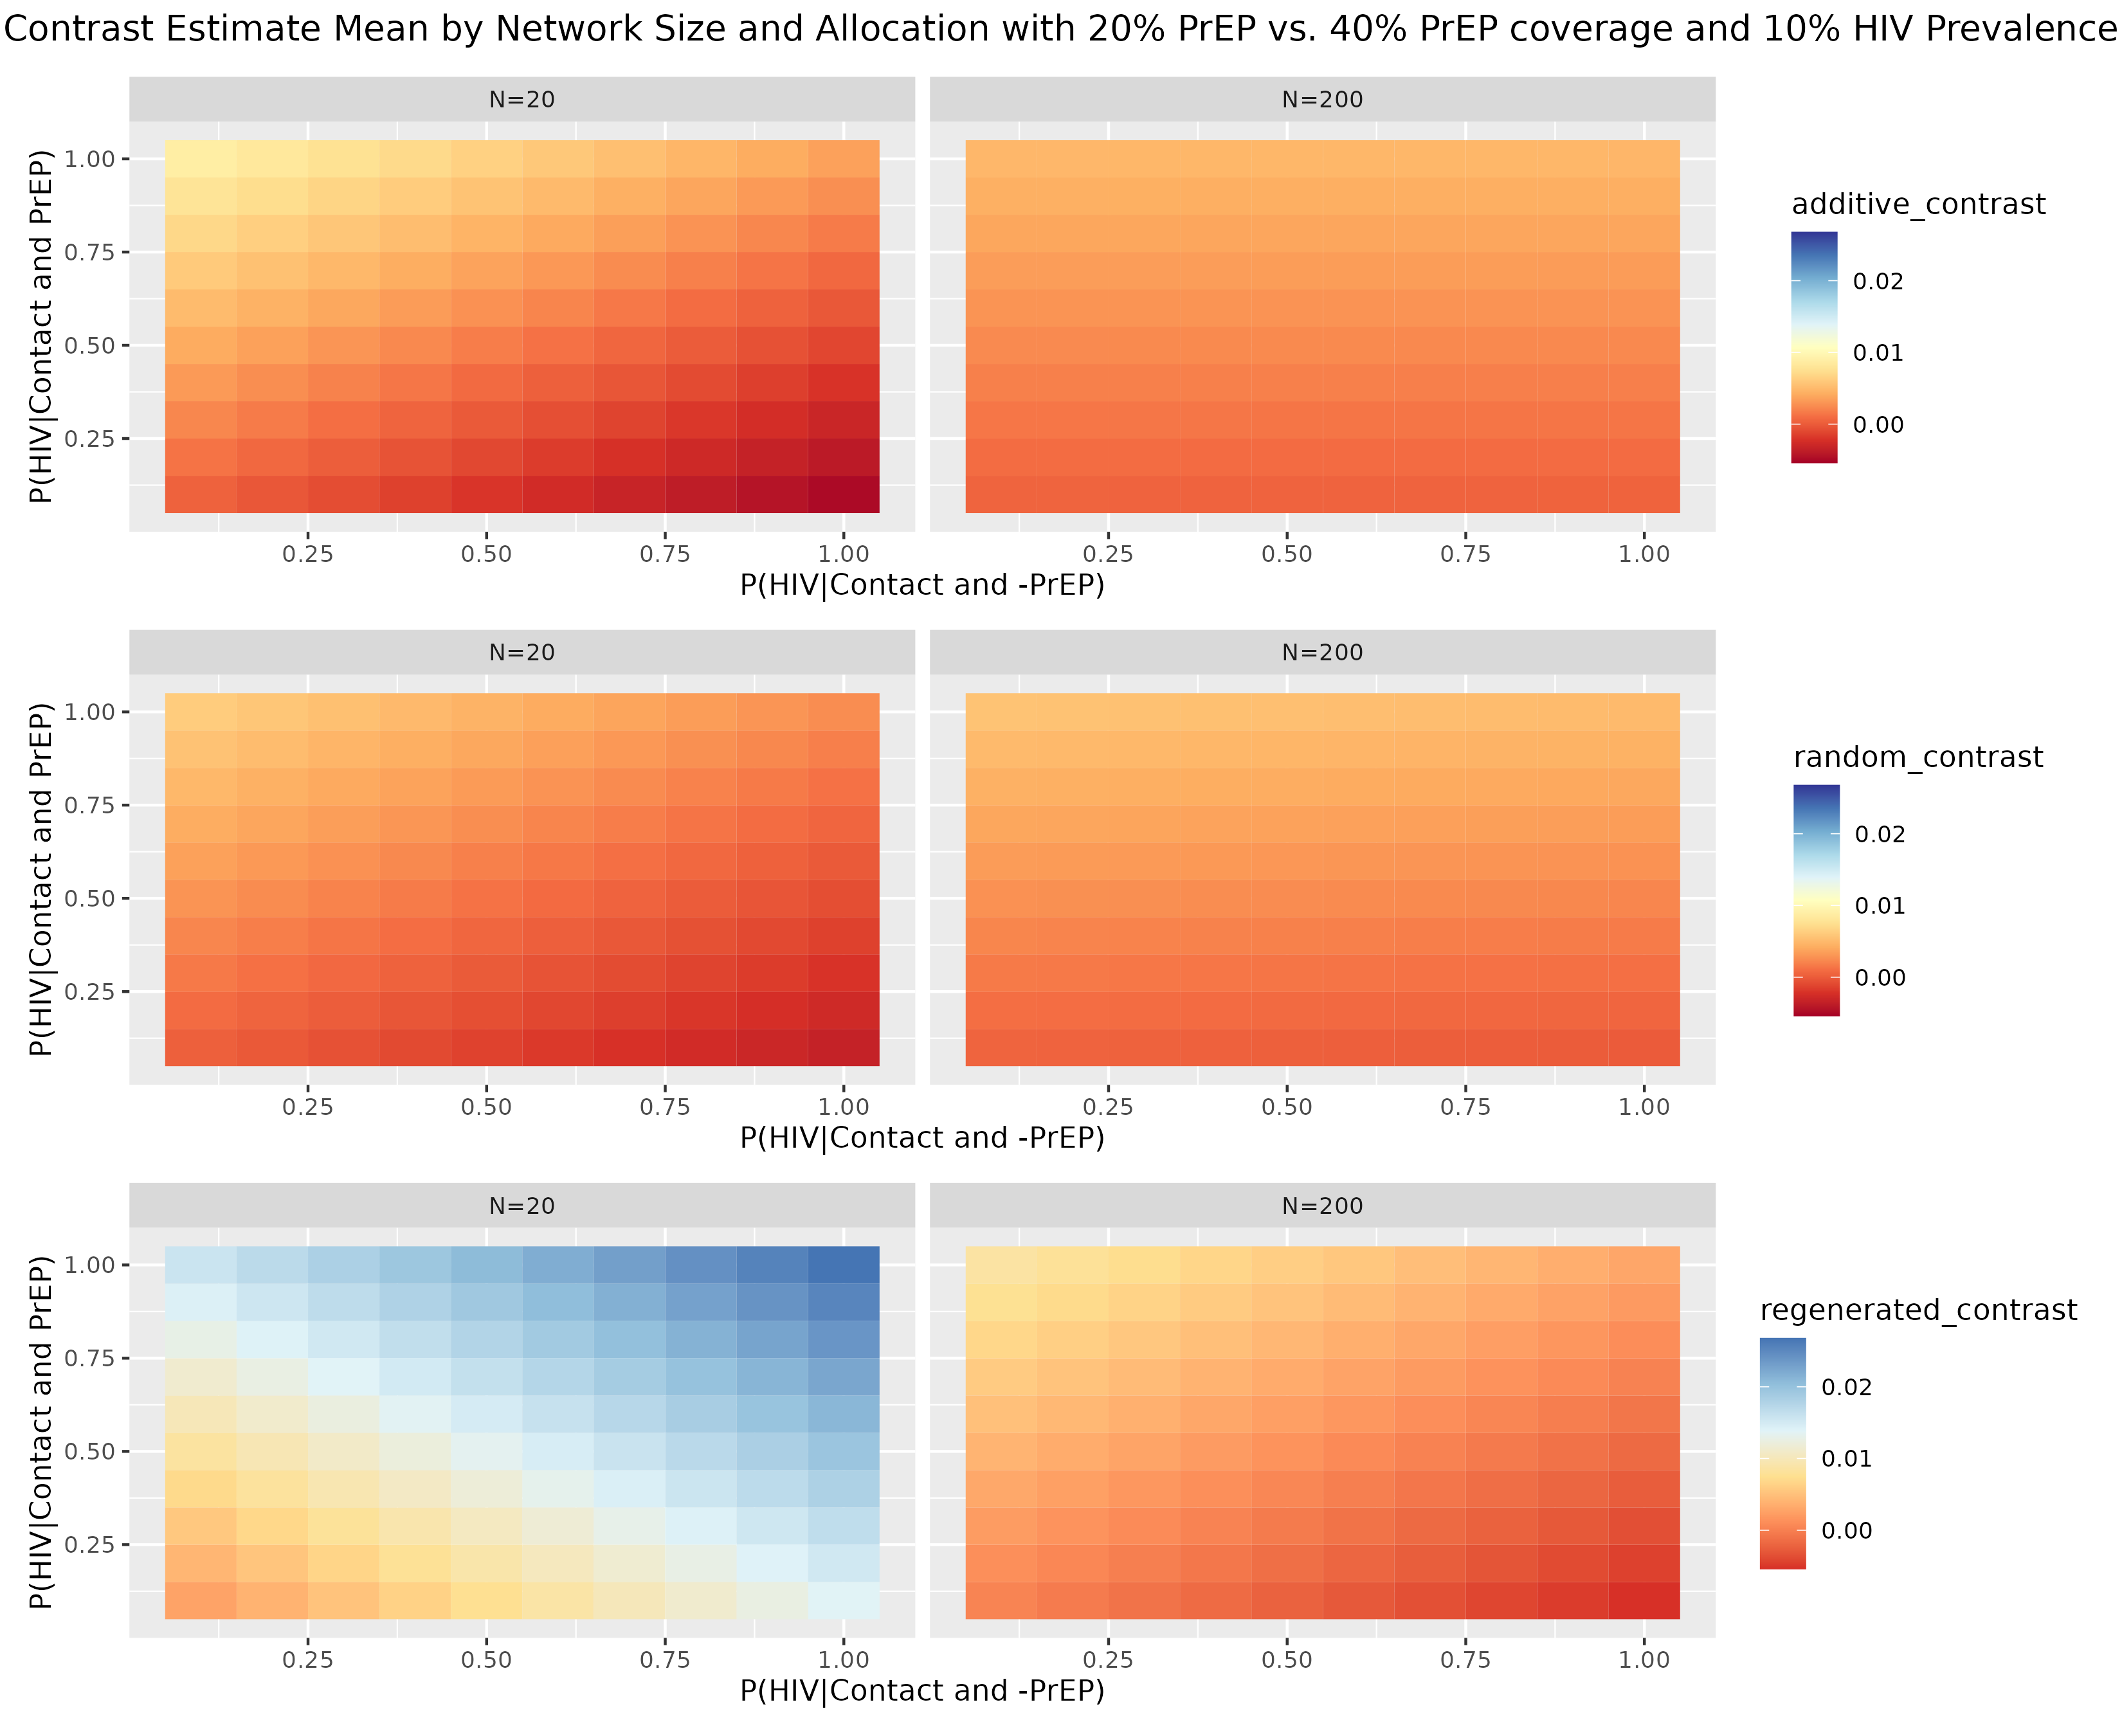
\includegraphics[width=\linewidth]{Corrected Figures/Network Size Mean Plot.png}
    \caption{Mean risk difference estimates comparing number of new infections when 40\% versus 20\% of uninfected nodes are treated with PrEP across varying levels of $\mathbb{P}\left[\text{HIV} \vert \neg \text{PrEP} \cap \text{Contact}\right]$ and $\mathbb{P}\left[\text{HIV} \vert \text{PrEP} \cap \text{Contact}\right]$, stratified by Network Size and using 200 simulation samples 
    From top to bottom: ``Additive" approach increases proportion on PrEP compared to a given network realization and given set of treated nodes; ``Random" approach compares PrEP allocation levels for a given network realization, without fixing the treated nodes; ``Regenerated" approach compares PrEP levels without fixing network realization or treated nodes. }
    \label{fig:Figure 7}
\end{figure}

We see similar patterns when we hold the network size fixed but vary the number of realizations simulated. The difference between the approaches here is most clearly visualized by a plot of the variance in risk difference estimate across all runs (Figure \ref{fig:Figure 8}). The variance in the risk difference estimates is smallest for the Additive approach, and largest for the Regenerated approach. Regardless of approach to simulation, the variance decreases as the number of simulation iterations increases.

\begin{figure}[H]
    \centering
    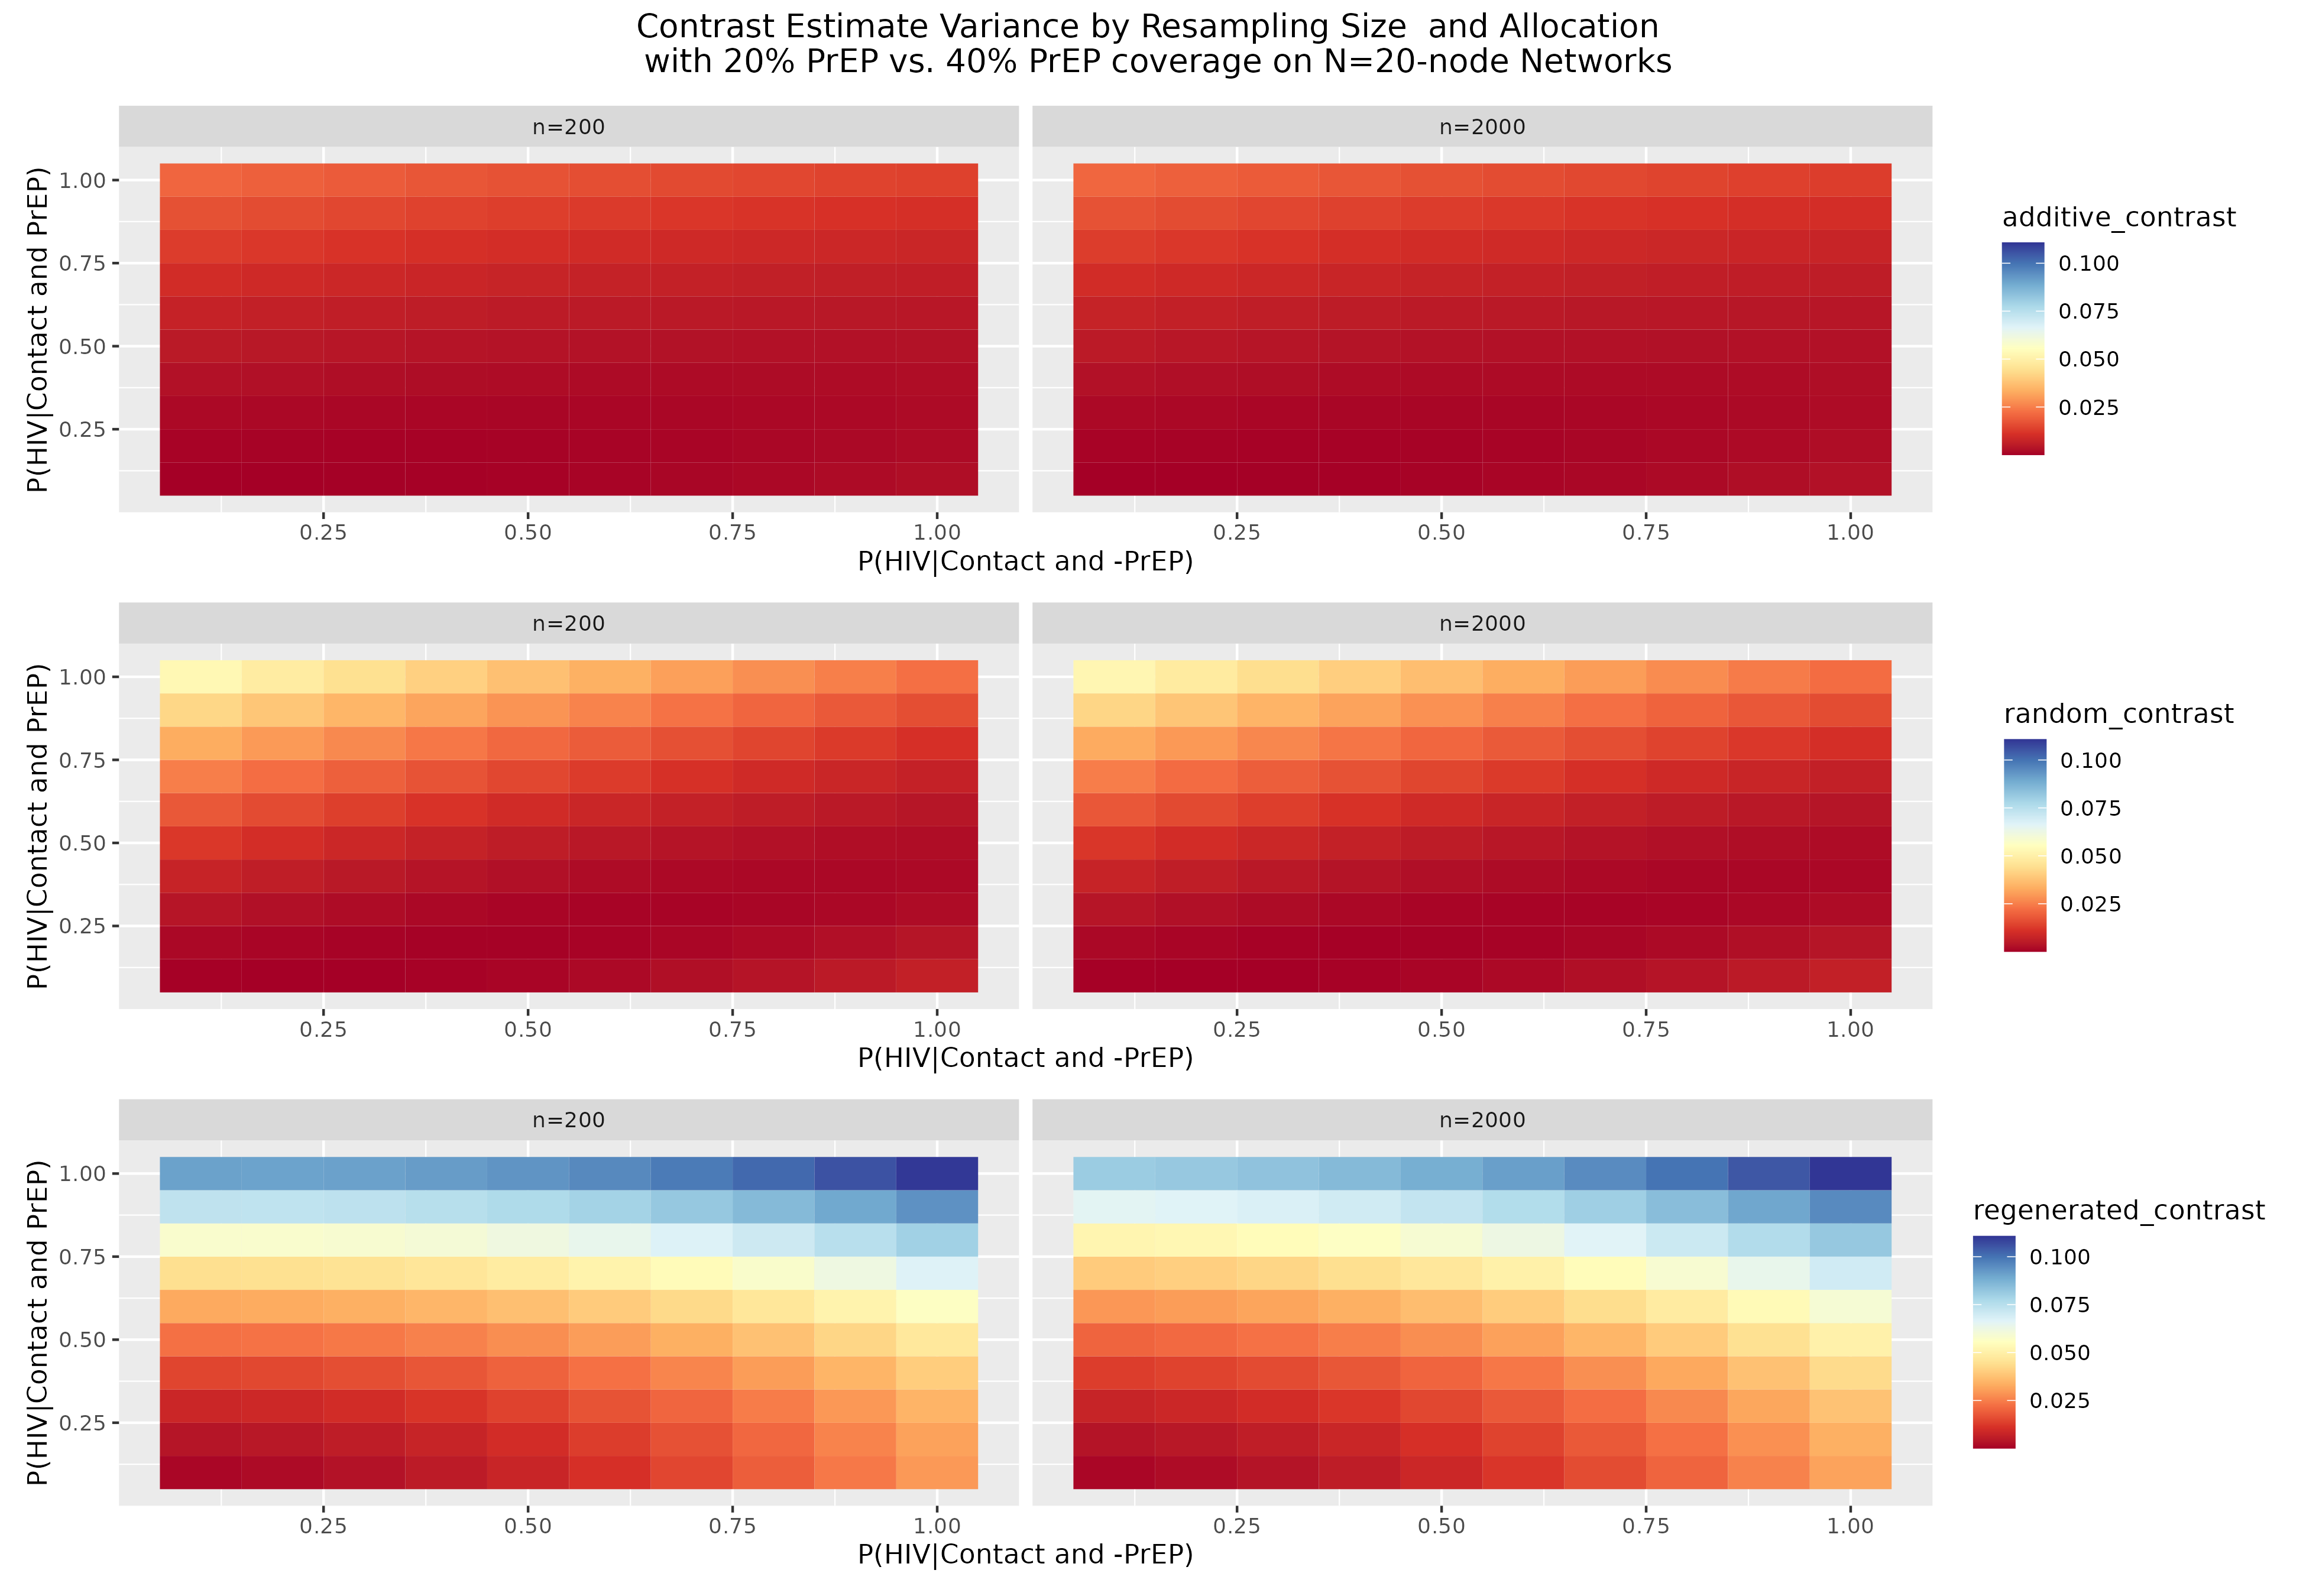
\includegraphics[width=\linewidth]{Corrected Figures/Resampling Size Variance Plot.png}
    \caption{Variance of risk difference estimates comparing number of new infections when 40\% versus 20\% of uninfected nodes are treated with PrEP across varying levels of $\mathbb{P}\left[\text{HIV} \vert \neg \text{PrEP} \cap \text{Contact}\right]$ and $\mathbb{P}\left[\text{HIV} \vert \text{PrEP} \cap \text{Contact}\right]$, stratified by number of simulations sampled when network size is 20 %%PLEASE ADD%%. 
    From top to bottom: ``Additive" approach increases proportion on PrEP compared to a given network realization and given set of treated nodes; ``Random" approach compares PrEP allocation levels for a given network realization, without fixing the treated nodes; ``Regenerated" approach compares PrEP levels without fixing network realization or treated nodes. }
    \label{fig:Figure 9}
\end{figure}

\subsubsection{Probabilities of infectious contact and infection given contact}
As described above, we anticipate that as either the proportion of individuals with an infectious contact or the proportion treated increases to the size of the uninfected network nodes, the proportion of network realizations in which at least one node has both treatment and an infectious contact will increase towards 100\%. However, at higher values of treatment and/or infectious contact, we might also expect to see greater variation in the \textit{number} of nodes with both treatment and an infectious contact across network realizations. This is what we see in the simulation -- comparing the estimated risk difference across increasing HIV infection prevalence (and thus increasing probability that any uninfected individual has an infectious contact), we see that the variance is relatively constant when using the Additive approach but very variable when using the Regenerated approach (Figure \ref{fig:Figure 10}.


\begin{figure}[H]
    \centering
    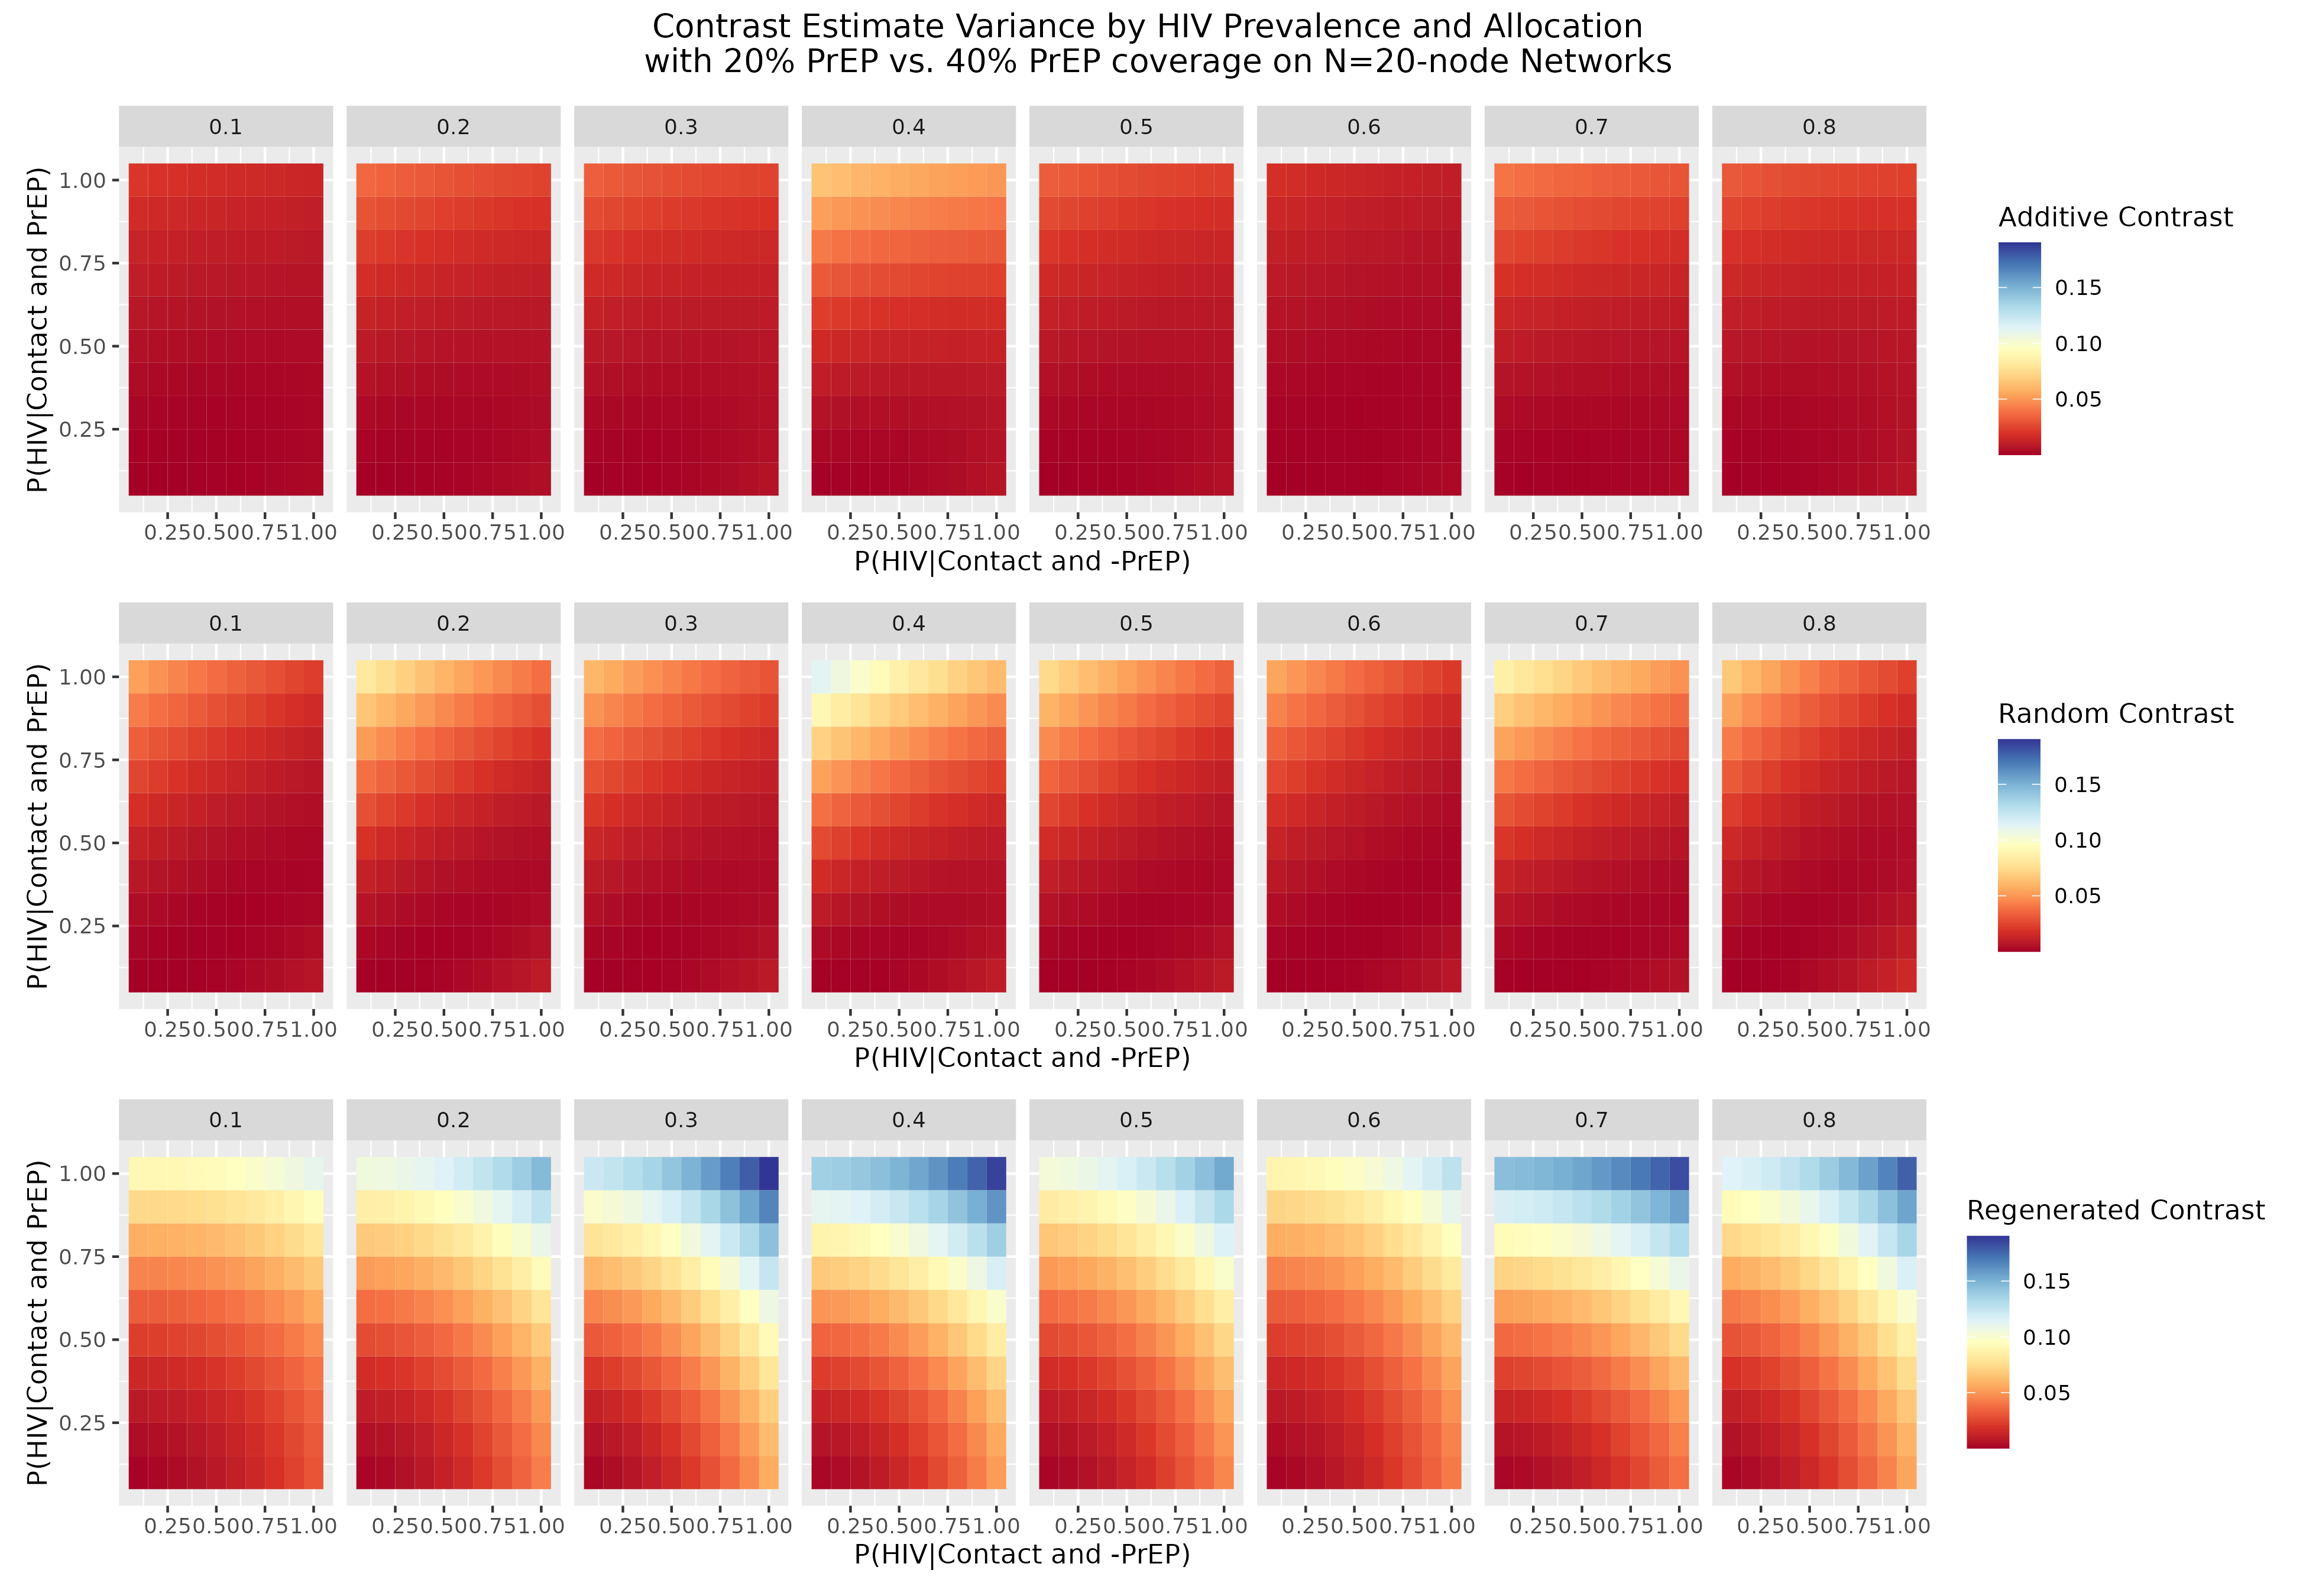
\includegraphics[width=\linewidth]{Corrected Figures/HIV Prevalence Variance Plot.png}
    \caption{Variance of risk difference estimates comparing number of new infections when 40\% versus 20\% of uninfected nodes are treated with PrEP across varying levels of $\mathbb{P}\left[\text{HIV} \vert \neg \text{PrEP} \cap \text{Contact}\right]$ and $\mathbb{P}\left[\text{HIV} \vert \text{PrEP} \cap \text{Contact}\right]$, stratified by starting HIV prevalence in the network with network size of 20 and 200 simulation samples.
    From top to bottom: ``Additive" approach increases proportion on PrEP compared to a given network realization and given set of treated nodes; ``Random" approach compares PrEP allocation levels for a given network realization, without fixing the treated nodes; ``Regenerated" approach compares PrEP levels without fixing network realization or treated nodes.}
    \label{fig:Figure 10}
\end{figure}


Likewise, when we hold the probability of infection given either PrEP (Figure \ref{fig:Figure 11}) or no PrEP (Figure \ref{fig:Figure 12}) constant and vary the other, we see that the estimated mean risk differences are much more consistent when using the Additive approach compared to the Regenerated approach. 


\begin{figure}[H]
    \centering
    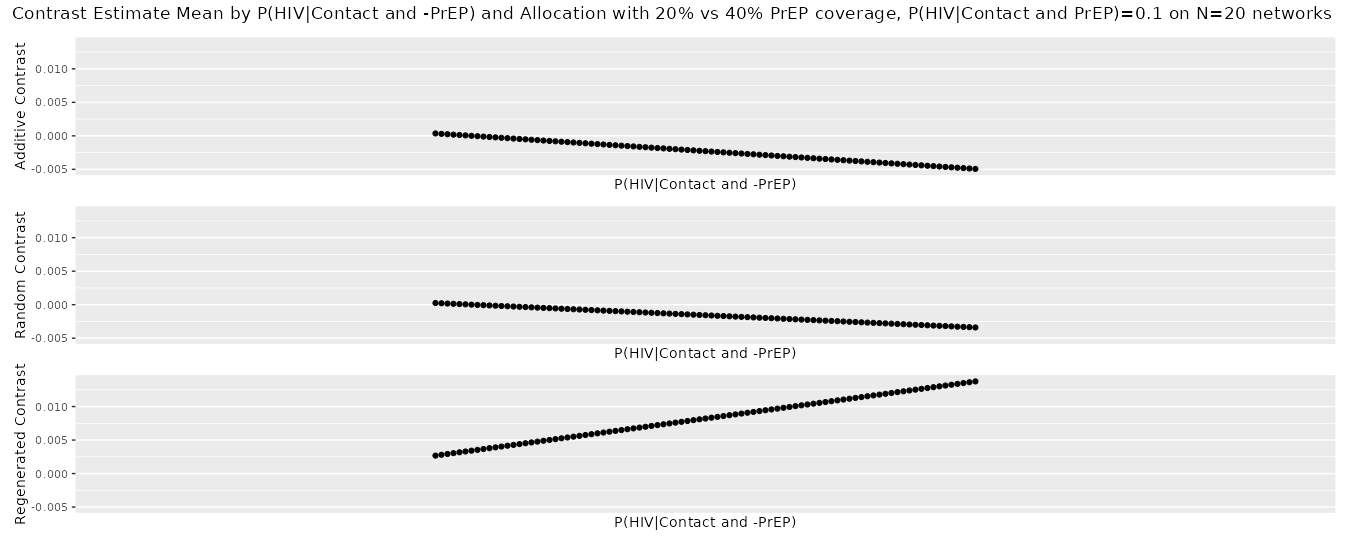
\includegraphics[width=\linewidth]{Corrected Figures/p1 Mean plots.png}
    \caption{Mean risk difference estimates comparing number of new infections when 40\% versus 20\% of uninfected nodes are treated with PrEP across varying levels of  $\mathbb{P}\left[\text{HIV } \vert \text {Contact } \cap \neg \text{ PrEP}\right]$ , with network size of 20,  200 simulation samples,  10\% HIV prevalence at baseline, and an 10 \% probability of infection given contact and PrEP.
    From top to bottom: ``Additive" approach increases proportion on PrEP compared to a given network realization and given set of treated nodes; ``Random" approach compares PrEP allocation levels for a given network realization, without fixing the treated nodes; ``Regenerated" approach compares PrEP levels without fixing network realization or treated nodes.}
    \label{fig:Figure 11}
\end{figure}

\begin{figure}[H]
    \centering
    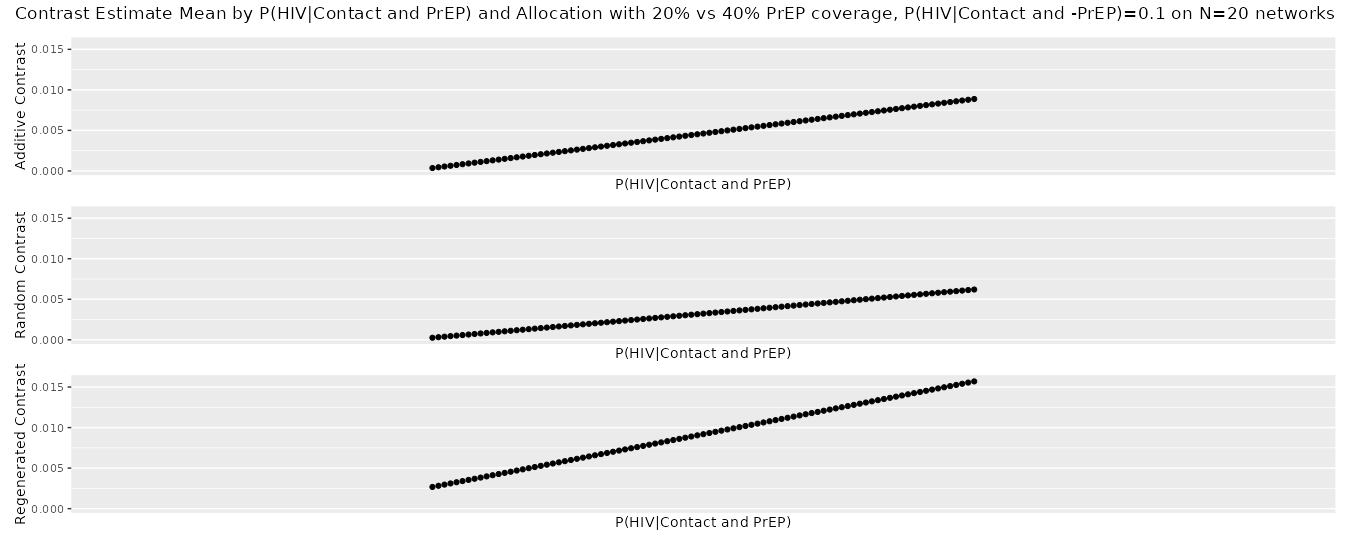
\includegraphics[width=\linewidth]{Corrected Figures/p2 Mean plots.png}
    \caption{
    Mean risk difference estimates comparing number of new infections when 40\% versus 20\% of uninfected nodes are treated with PrEP across varying levels of  $\mathbb{P}\left[\text{HIV } \vert \text{ PrEP}\right]$, with network size of 20 ,  200 simulation samples,  10\% HIV prevalence at baseline, and an 10 \% probability of infection given contact and no PrEP.
     From top to bottom: ``Additive" approach increases proportion on PrEP compared to a given network realization and given set of treated nodes; ``Random" approach compares PrEP allocation levels for a given network realization, without fixing the treated nodes; ``Regenerated" approach compares PrEP levels without fixing network realization or treated nodes.}
    \label{fig:Figure 12}

\end{figure}


\subsubsection{Network model type}
The patterns observed with the Erdos-Renyi network graphs were even more pronounced using the Barabasi-Albert scale-free model,  but less so with the Watts-Strogatz Small-world model (Figure \ref{fig:Figure 13}). Likely this is because of less variation in allowed contact patterns between WS network realizations, given the requirement of a fully-connected graph. 


\begin{figure}[H]
    \centering
    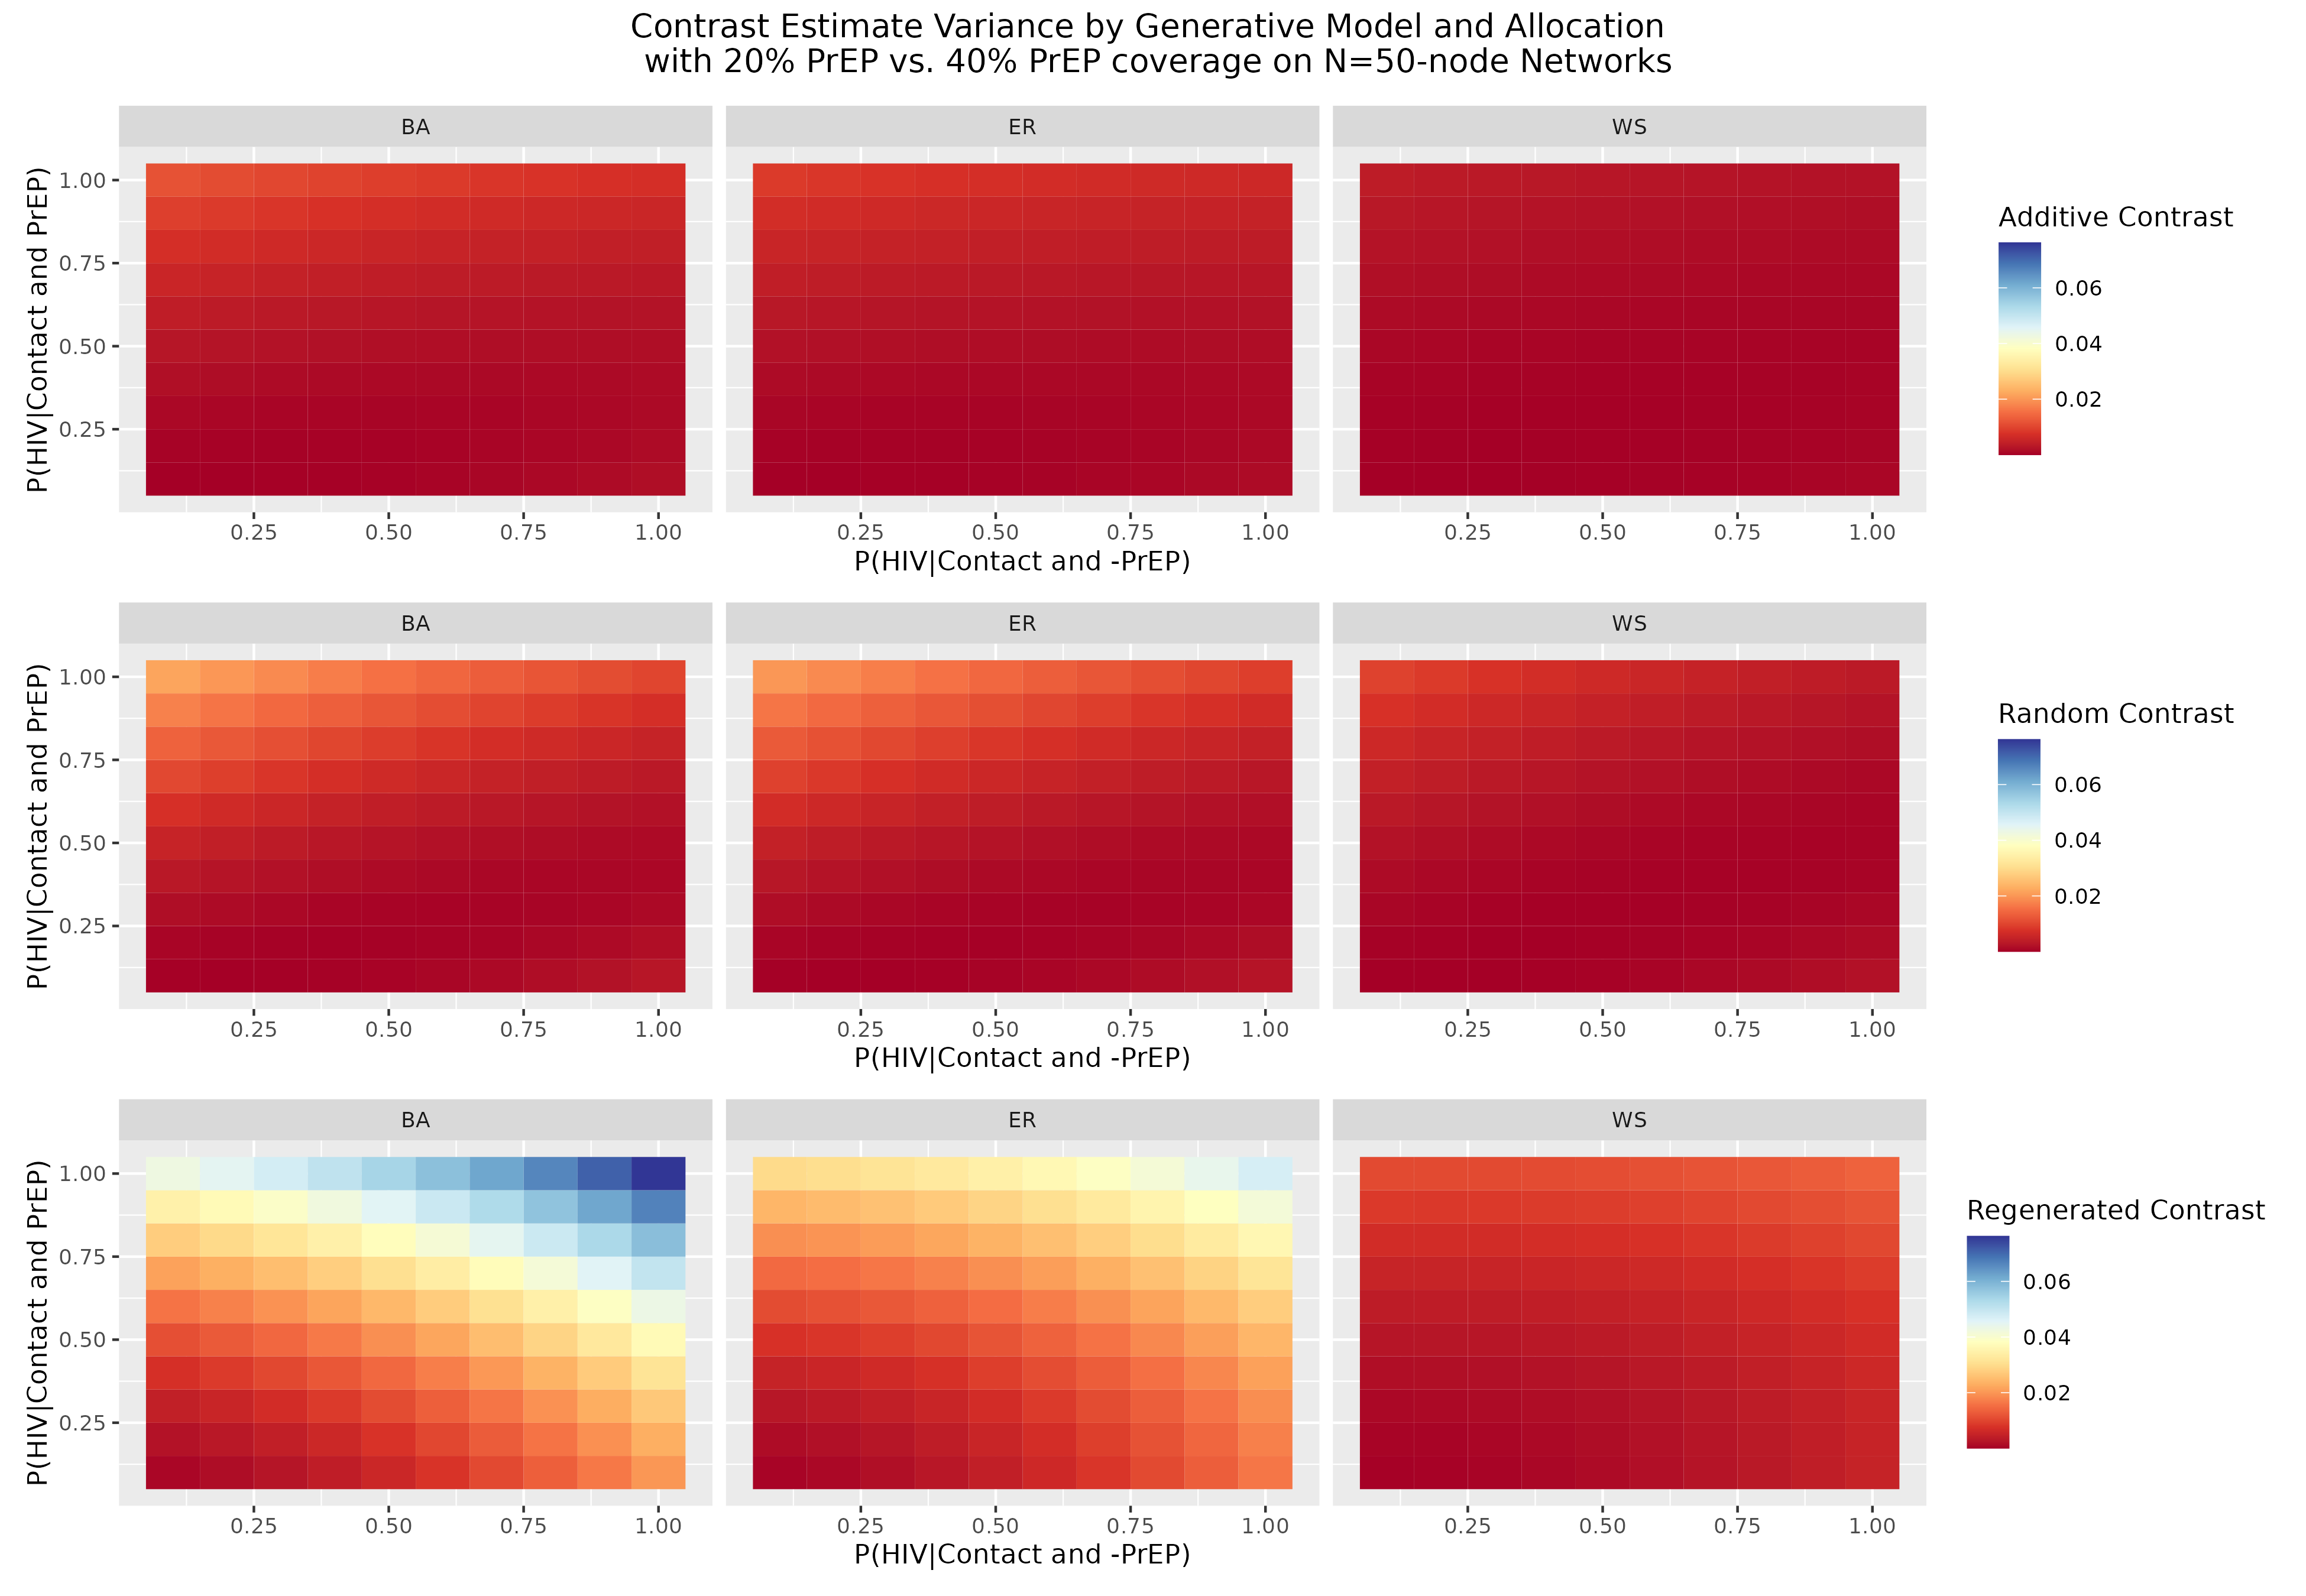
\includegraphics[width=\linewidth]{Corrected Figures/Generative Model Variance Plot.png}
    \caption{Variance of risk difference estimates comparing number of new infections when 40\% versus 20\% of uninfected nodes are treated with PrEP across varying levels of $\mathbb{P}\left[\text{HIV} \vert \neg \text{PrEP} \cap \text{Contact}\right]$ and $\mathbb{P}\left[\text{HIV} \vert \text{PrEP} \cap \text{Contact}\right]$, stratified by Network Generative Model with a Network Size of 50 and using 200 simulation samples %%PLEASE ADD%%. 
    From left to right, ``BA" the Barabási–Albert scale-free model, ``ER" the Erdős–Rényi Random Graph model, ``WS" the Watts-Strogatz Small-World model. From top to bottom: ``Additive" approach increases proportion on PrEP compared to a given network realization and given set of treated nodes; ``Random" approach compares PrEP allocation levels for a given network realization, without fixing the treated nodes; ``Regenerated" approach compares PrEP levels without fixing network realization or treated nodes. 
    }
    \label{fig:Figure 13}
\end{figure}


\section{Discussion}

 When estimating causal effects using network-based simulation models, the exact pattern of network contacts is a potential source of bias because it determines the outcome and the potential range of causal effects under different treatment patterns on that realization. Whenever a simulation study must use a finite number of network realizations, but does not have a specific empiric network structure of interest, it is important that the each counterfactual contrast be estimated on every network realization to reduce the impact of this bias. 

 In both our simplified example and our more complex simulations, we see that this potential for bias can affect our estimates when an inappropriate choice of network simulation approach is used.  For all model parameters considered, our simulations showed evidence of effect modification of the relationship between risks of HIV given infectious contact with and without PrEP treatment. This effect modification is the source of the bias in the estimated average overall effects when we do not estimate counterfactuals conditional on network realization. 

 In our simulations, the impact of network parameters on the amount of bias aligned with our expectations based on the probability of informative networks. The variance estimates appear to converge for sufficiently large resampling sizes. In addition, the effect estimates tend toward the null as network sizes increases, at least across one order of magnitude. Larger magnitudes could not be implemented due to computational constraints. We also see an impact of transmission-related parameters, including per-contact infectivity and baseline infection prevalence, on the amount of bias. These simulation results agree with our expectations regarding the effect of proportion with infectious contacts and proportion receiving treatment on the potential for uninformative network realizations. 

We focused on examples that considered only the first time step of the simulation and as a result the impact of interference in our analyses was minimal. Because of this, we chose to present only the average overall effect estimates. However it is important to be aware that the bias described here is not restricted to the average overall effect. In fact, all causal effects for depending happenings are expected to be vulnerable to this bias. As time in the simulation increases, there will generally be an increase in the number of people infected and thus the proportion of the population who are uninfected and treated and/or have an infectious contact will change. This will change the distribution of informative network realizations (those where at least one treated individual has an infectious contact), and the amount of expected bias when not conditioning on network-realization will thus evolve over time. 

Overall, when network-based causal effects are of interest and the true network structure(s) is unknown so that the network must be simulated, we recommend that every simulated realization of the network be subjected to all treatment patterns under study, so that network-specific causal effects can be estimated for each realization and then pooled across all simulated network realizations. This approach will ensure the smallest variance and least bias in the results, for a given set of parameters, and will often allow smaller or fewer network simulations to be run. In the rare case where the exact structure of the network of interest is known, the same approach is appropriate except that the resulting causal effect estimate will be the average network-specific causal effect, not the average causal effect across all networks with the given parameter set.




\newpage

\bibliographystyle{unsrt}
\bibliography{references}
\newpage


\appendix
\counterwithin{figure}{section}
\section{Appendix 1: Derivation of  \textit{P}}
\label{Appendix 1}
Here we describe the details of the definition for $P$, the probability of at least one node $i$ in a network being assigned to treatment with at least one infectious contact for a given network structure $j$ and a given treatment $a$ or $a*$.

In the following calculation, we will be using the notation $f(x)\approx g(x)$ to mean that $f(x)=\Theta(g(x))$. Big theta notation is used to denote that there exists $N$ such that for $x>N$, there exist constants $c$ and $d$ such that:

 $$c\cdot g(x)< f(x) < d \cdot g(x) $$

It is easy to show that if $0<a<x<b$ and $0<c<y<d$, then $-d<-y<-c$ and $\frac{1}{d}<\frac{1}{y}<\frac{1}{c}$.  Therefore, the following are true:
\begin{enumerate}
\item $ac<xy<bd$
\item $0<\frac{a}{d}<\frac{x}{y}<\frac{b}{c}$
\end{enumerate}

It follows that if $f_1(x)=\Theta{\left(g_1(x)\right)}$ and $f_1(x)=\Theta{\left(g_2(x)\right)}$ where $f_1$,$f_2$, $g_1$ and $g_2$ are strictly positive then:
\begin{enumerate}
\item $f_1(x)f_2(x)=\Theta{\left(g_1(x)g_2(x)\right)}$
\item $\frac{f_1(x)}{f_2(x)}=\Theta{\left(\frac{g_1(x)}{g_2(x)}\right)}$
\end{enumerate}

In our notation, this means:
\begin{enumerate}
     \item $f_1(x)f_2(x)\approx g_1(x)g_2(x)$ 
     \item $\frac{f_1(x)}{f_2(x)}\approx \frac{g_1(x)}{g_2(x)}$.
\end{enumerate}


Additionally, we will be using this version of Stirling's approximation,

$$n!= \Theta\left(\sqrt{2\pi n}\left(\frac{n}{e}\right)^n \right)$$

Now, assume that $N$ is the network population at a given time point, that $k<N$ is the number of individuals that receive treatment, and that $n<N$ is the number of individuals with an infectious contact. Then, there are $\binom{N}{k}$ unique network configurations.
 
The expected number of unique network configurations in which all treated individuals have no infectious contacts (and thus a contribution of 0 to the effect estimate) is then given by $\binom{N-n}{k}$. Then, the proportion of network configurations in which at least one treated individual has at least one infectious contact is 
\begin{equation} 
\frac{{\binom{N}{k}}-{\binom{N-n}{k}}}{{\binom{N}{k}}}=1-\frac{{\binom{N-n}{k}}}{{\binom{N}{k}}}  \nonumber
\end{equation}
Expanding the RHS gives:
\begin{equation}
1-\frac{\left(N-n\right)!\left(N-k\right)!}{k!\left(N-n-k\right)!} \nonumber
\end{equation}
Using Stirling's Approximation as appropriate,
\begin{equation}
\approx 1-\frac{\sqrt{2\pi\left(N-n\right)}\left(\frac{N-n}{e}\right)^{N-n}\sqrt{2\pi\left(N-k\right)}\left(\frac{N-k}{e}\right)^{N-k}}{\sqrt{2\pi N}\left(\frac{N}{e}\right)^{N}\sqrt{2\pi \left(N-n-k\right)}\left(\frac{N-n-k}{e}\right)^{N-n-k}}     \nonumber
\end{equation}
%see page 2b
We can then make the following approximations and simplifications:
\begin{equation}
    \frac{\sqrt{2\pi \left(N-n\right)}}{\sqrt{2\pi N}}=\sqrt{\frac{N-n}{N}}\approx 1 \text{ for } N>>n \nonumber\\
    \end{equation}
    \begin{equation}
    \frac{\sqrt{2 \pi \left(N-k\right)}}{\sqrt{2 \pi \left(N-n-k\right)}}\approx 1 \nonumber
\end{equation}
    \begin{align}
    \frac{\left(\frac{\left(N-n\right)}{e}\right)^{N-n}}{{\left(\frac{N}{e}\right)^{N}}}&=\frac{\left(N-n\right)^{N-n}e^{N}}{N^{N}e^{N-n}} \nonumber\\
     &=\frac{e^{n}}{N^{n}}\left(\frac{N-n}{N}\right)^{N-n} \nonumber\\
     &=\frac{e^{n}}{N^{n}}\left(1-\frac{n}{N}\right)^{N-n} \nonumber\\
     &=\frac{e^{n}}{N^{n}}\frac{\left(1-\frac{n}{N}\right)^{N}}{\left(1-\frac{n}{N}\right)^{n}} \nonumber\\
     &\approx \frac{e^{n}}{N^{n}}\lim_{N \to \infty}\frac{\left(1-\frac{n}{N}\right)^{N}}{\left(1-\frac{n}{N}\right)^{n}} \nonumber\\
     &=\frac{e^{n}}{N^{n}}\frac{e^{-n}}{1^{n}} \nonumber\\
     &=\frac{1}{N^{n}} \nonumber
\end{align}
\begin{align}
    \frac{\left(\frac{N-k}{e}\right)^{N-k}}{\left(\frac{N-n-k}{e}\right)^{N-n-k}}&\stackrel{M\coloneqq N-k}{=}\frac{\left(\frac{M}{e}\right)^{M}}{\left(\frac{M-n}{e}\right)^{M-n}}\to M^{n} \nonumber\\
    \frac{M^{n}}{N^{n}}&=\left(\frac{N-k}{N}\right)^{n}\nonumber
\end{align}
simplifying as appropriate gives
\begin{align}
    & \approx 1- \frac{\left(N-n\right)^{N-n}\left(N-k\right)^{N-k}}{N^{N}\left(N-n-k\right)^{N-n-k}} \nonumber\\
    &= 1- N^{-N}\left(\frac{N-n}{N}\right)^{N-n}\left(N-k\right)^{n}\left(\frac{N-k}{N-n-k}\right)^{N-n-k} \nonumber\\
    &=1-\left(\frac{N^{n}\left(1-\frac{n}{N}\right)^{N}\left(N-k\right)^{n}}{\left(1-\frac{n}{N}\right)^{n}}\right)\left(\frac{N-n-k}{N-k}\right)^{k+n-N} \nonumber\\
    &=1-\left(\frac{N^{-n}e^{-n}\left(N-k\right)^{n}}{1}\right)\left(\frac{\left(1-\frac{n}{N-k}\right)^{n}}{\left(1-\frac{n}{N-k}\right)^{N-k}}\right) \nonumber\\
    &=1-\frac{N^{-n}\left(N-k\right)^{n}e^{-n}}{e^{-n}} \nonumber\\
    &=1-\frac{\left(N-k\right)^{n}}{N^{n}} \nonumber\\
    &=1-\left(\frac{N-k}{N}\right)^{n}.\nonumber
\end{align}

\newpage
\section{Appendix 2: Summary Statistics}
\label {Appendix 2}
\subsection{Definitions}
\begin{definition}[Connected Components]
A connected component of a graph $G=(V,E)$ is a subgraph $G'=(V' \subseteq V,E' \subseteq E)\subseteq G$ such that there exists a path between any two nodes in $V'$.
\end{definition}
\begin{definition}[Betweenness Centrality]
The Betweenness Centrality for a node $v$ is given by: $$g(v)=\sum_{s\neq t\neq v}\frac{\sigma_{s,t}(v)}{\sigma_{s,t}},$$ where $\sigma(s,t)$ is  the number of shortest paths between node s and node t, and  $\sigma_{s,t}(v)$ is the number of shortest paths between node $s$ and node $t$ containing the node $v$ \cite{barabasi_network_2016}.
\end{definition}
\begin{definition}[Edge Density]
The (edge) density of a graph is the proportion of possible edges between nodes
that are actually present in the graph.
\end{definition}
\begin{definition}[Geodesic distance]
The geodesic distance between two nodes is the length of the shortest path between them.
\end{definition}
\begin{definition}[Graph diameter]
The diameter of a graph or graph component is the largest path length between any two nodes is the graph (component).
\end{definition}
\begin{definition}[Transitivity]
Transitivity is the proportion of closed triangles in a graph.
\end{definition}
\begin{definition}[$k$-core decomposition]
A $k$-core of a graph is a subgraph in which all nodes are connected to at least $k$ other nodes in the subgraph.
\end{definition}
\subsection{Results by Network Model}
\begin{figure}[H]
    \centering
    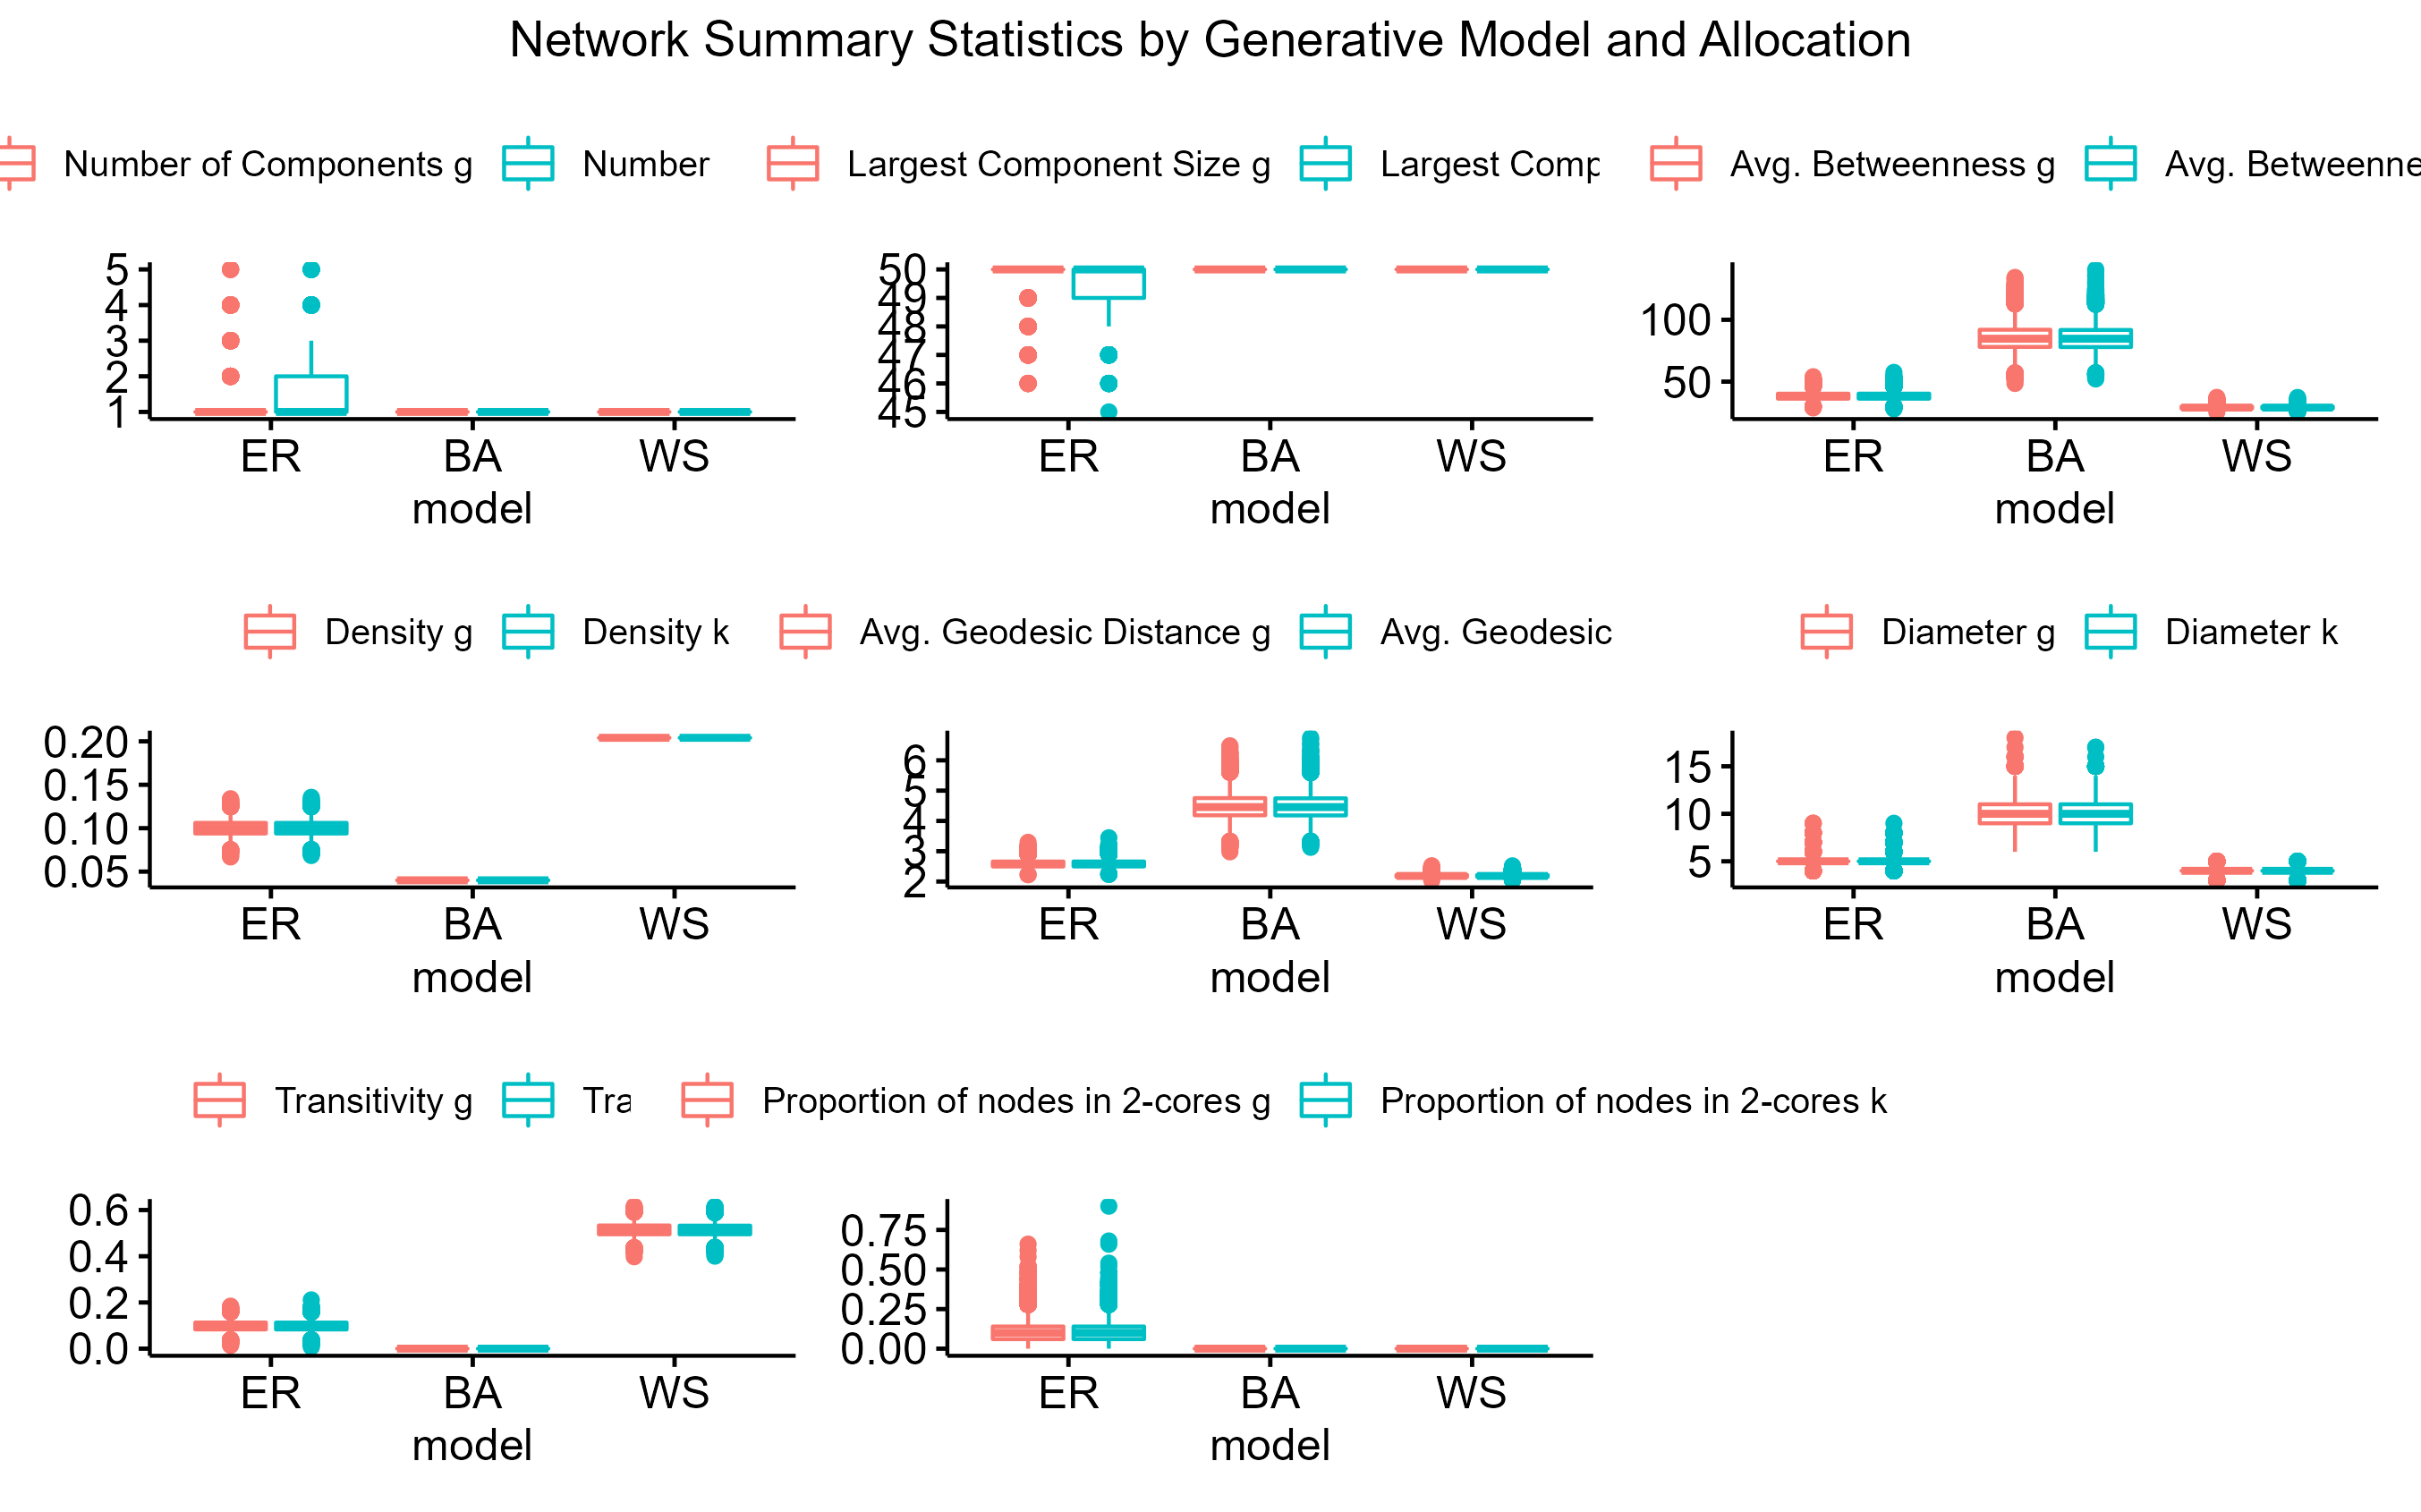
\includegraphics[width=\linewidth]{Original Figures/Network Summary Statistics.png}
    \caption{Select Network Summary Statistics by Network Generative Model}
    \label{fig:Figure B1}
\end{figure}
% \section{Expanded Effect Definitions}

% \subsection{Overall Effect}
%As before,  let $Y$ be the outcome of interest, $a$, $a∗$ be counterfactuals of treatment strategy $A$, and $j$ be an identifier of a network.
% The Overall Effect (OE) at timestep $t$ of counterfactual PrEP allocation $a>a*$ is the difference of the marginal population average potential outcomes under $a$ and $a*$:
% \begin{equation}
%     OE(a)=\mathbb{E} [Y_{t}^{a}]-\mathbb{E}[Y_{t}^{a*}].
% \end{equation}


\newpage
\section{Algorithm for simulating the average overall effect on networks}
\label{Appendix 3}

    \begin{enumerate}
\item In each simulation iteration, let $G_{\text{control}}=\left(V_{\text{control}},E_{\text{control}}\right)$ be the ``control" network graph, with $\vert V_{\text{control}}\vert \eqqcolon N_{\text{control}}$. The vertex attributes of $V_{\text{control}}$ are initialized to one of three states: 
\begin{itemize}
        \item  $N_{HIV}(V_{\text{control}})=N_{\text{control}}p_{hiv}$ nodes are initialized to the  ``infectious" state.
        \item $N_{PrEP_{1}}\left(V_{\text{control}}\right)=\left[N_{\text{control}}-N_{HIV}\left(V_{\text{control}}\right)\right]p_{PrEP_{1}}$ nodes are initialized to the ``treated,susceptible" state. 
        \item The remaining $N_{\text{control}}-\left[N_{HIV}\left(V_{\text{control}}\right)+N_{PrEP_{1}}\left(V_{\text{control}}\right)\right]$ nodes are initialized to the ``untreated, susceptible" state.
    \end{itemize}
    \item The set $IC(V_{\text{control}})$ of susceptible nodes with at least one infectious contact is identified from each node's neighborhood.
    \item The probability of HIV given treatment in the control scenario, $\mathbb{P}(\text{HIV} \vert \text{PrEP})_{\text{control}}$ is computed:
    \begin{enumerate}
     
    \item We compute $\mathbb{P}\left( \text{PrEP} \cap \text{Infectious contact}\right)$ as the proportion of the treated set  $T(V_{\text{control}})$ that have an infectious contact: \begin{equation}
        \mathbb{P}\left( \text{PrEP} \cap \text{Infectious contact}\right)=\frac{\vert IC\left(V_{\text{control}}\right) \bigcap \left({T\left(V_{\text{control}}\right)}\right)\vert}{\vert T\left(V_{\text{control}}\right)\vert}.\nonumber
    \end{equation}
    \item The probability $\mathbb{P}\left(\text{HIV} \vert \text{PrEP}\right)_{\text{control}}$ is then 
    \begin{equation}
        \mathbb{P}\left(\text{HIV} \vert \text{PrEP}\right)_{\text{control}}=\mathbb{P}\left(\text{HIV} \vert \text{PrEP} \cap \text{Infectious Contact}\right) \mathbb{P}\left(\text{PrEP} \cap \text{Infectious Contact}\right)\nonumber
    \end{equation}
    \end{enumerate}
    \item We then similarly compute the probability of HIV given no treatment in the control scenario, $\mathbb{P} \left(\text{HIV} \vert \neg \text{PrEP}\right)_{\text{control}}$:
    \begin{enumerate}
    \item We compute $\mathbb{P}\left(\neg \text{PrEP} \cap \text{Infectious Contact} \right)  $ as the proportion of untreated susceptible nodes that have an infectious contact:
    \begin{equation}
        \mathbb{P}\left(\neg \text{PrEP} \cap \text{Infectious Contact} \right)=\frac{\vert IC\left(V_{\text{control}}\right) \bigcap \left({T'\left(V_{\text{control}}\right)}\right)\vert}{\vert T'\left(V_{\text{control}}\right)\vert},\nonumber
    \end{equation}

    where $T'\left(V_{\text{control}}\right)$ denotes the set of untreated susceptible nodes.
    \item The probability $\mathbb{P}\left(\text{HIV} \vert \neg \text{PrEP}\right)_{\text{control}}$ is then
    \begin{equation}
        \mathbb{P}\left(\text{HIV} \vert \neg \text{PrEP}\right)_{\text{control}}=\mathbb{P}\left(\text{HIV} \vert \neg \text{PrEP} \cap \text{Infectious Contact}\right) \mathbb{P}\left( \neg \text{PrEP} \cap \text{Infectious Contact}\right).\nonumber
    \end{equation}
    \end{enumerate}
    \item For the ``random" and ``additive" $\text{PrEP}_{2}$ treatment allocation  scenarios, the topology of $G_{\text{control}}$ is fixed, but treatment attributes on the vertex set are varied. 
    \begin{enumerate}
        \item For the ``random" $\text{PrEP}_{2}$ scenario, the infectious nodes from the control scenario are fixed, but the treatment set is instead a randomly selected $N_{\text{control}}PrEP_{2}$ nodes.
        %check me %
        \item For the ``additive" scenario, the infectious nodes are fixed, with the treated set $T\left(V_{\text{additive}}\right)$ contains the original treated nodes in addition to $\left[N_{\text{control}}-N_{HIV}-N_{PrEP1}\right]PrEP_{2}$ treated nodes.
    \end{enumerate}
    \item For the ``regenerated" treatment scenario, a new graph $G_{\text{regenerated}}=\left(V_{ \text{regenerated}},E_{\text{regenerated}}\right)$ with new attributes on the vertex set is generated.
    \begin{itemize}
        \item $N_{HIV}\left(V_{\text{regenerated}}\right)p_{hiv}$ nodes are assigned to the ``infectious" state.
        \item $N_{PrEP_{2}}\left(V_{\text{regenerated}}\right)=\left[N_{\text{regenerated}}\left(V_{\text{regenerated}}\right)-N_{HIV}\left(V_{\text{regenerated}}\right)\right]p_{PrEP_{2}}$ nodes are assigned to the ``susceptible, treated" state. 
    \end{itemize}
    \item The probabilities of infection with and without treatment are then computed similarly to the control scenario.
    \item The combined probability of HIV is computed, given each PrEP coverage and allocation
    \item The contrast estimate between each of the counterfactual allocations (``random", ``additive", ``regenerated") and the control are computed as the difference  between each of these combined probabilities and that for the control.
    \item These simulations are repeated $n_{sim}$ times and the means of these contrast estimates are computed.
\end{enumerate}


\newpage
\section{Example Annotated Networks for all Generative Models}
\label{sec: D}
This appendix reproduces example networks for all generative models, demonstrating the relationship between the control network and the random and additive simulation approach for the intervention networks, compared to the regenerated network approach.

\begin{figure}
    \centering
    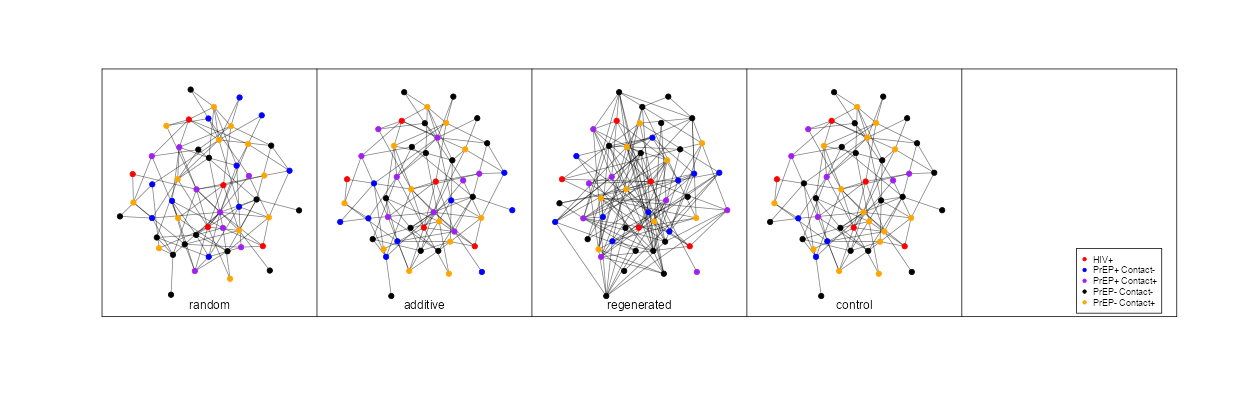
\includegraphics[width=\linewidth]{Original Figures/ER Network Example.png}
    \caption{Annotated Example ER Network showing color-coded treatment and disease states by network (control vs. regenerated) and allocation strategy(control vs. random, additive)}
    \label{fig: D1}
\end{figure}
\begin{figure}[H]
    \centering
    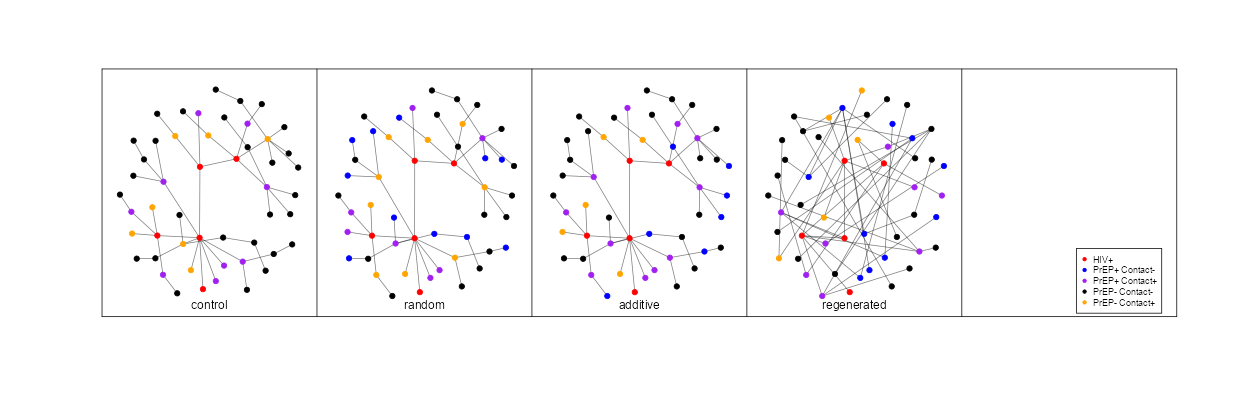
\includegraphics[width=\linewidth]{Original Figures/BA Network Example.png}
    \caption{Annotated Example BA Network showing color-coded treatment and disease states by network (control vs. regenerated) and allocation strategy(control vs. random, additive)}
    \label{fig: D2}
\end{figure}
\begin{figure}[H]
    \centering
    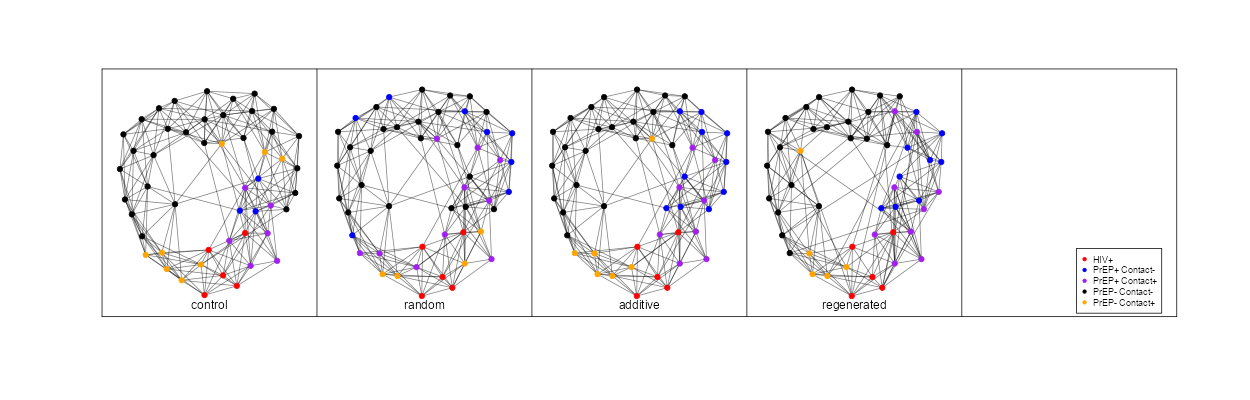
\includegraphics[width=\linewidth]{Original Figures/WS Network Example.png}
    \caption{Annotated Example WS Network showing color-coded treatment and disease states by network (control vs. regenerated) and allocation strategy (control vs. random, additive)}
    \label{fig: D3}
\end{figure}

\newpage

\section{Simulation model results across all input parameter and model type variations}
\label{sec: F}

\subsection{Erdős–Rényi  Random Graph Models}

\subsubsection{Effect Modification by Network Size}
\begin{figure}[H]
    \centering
    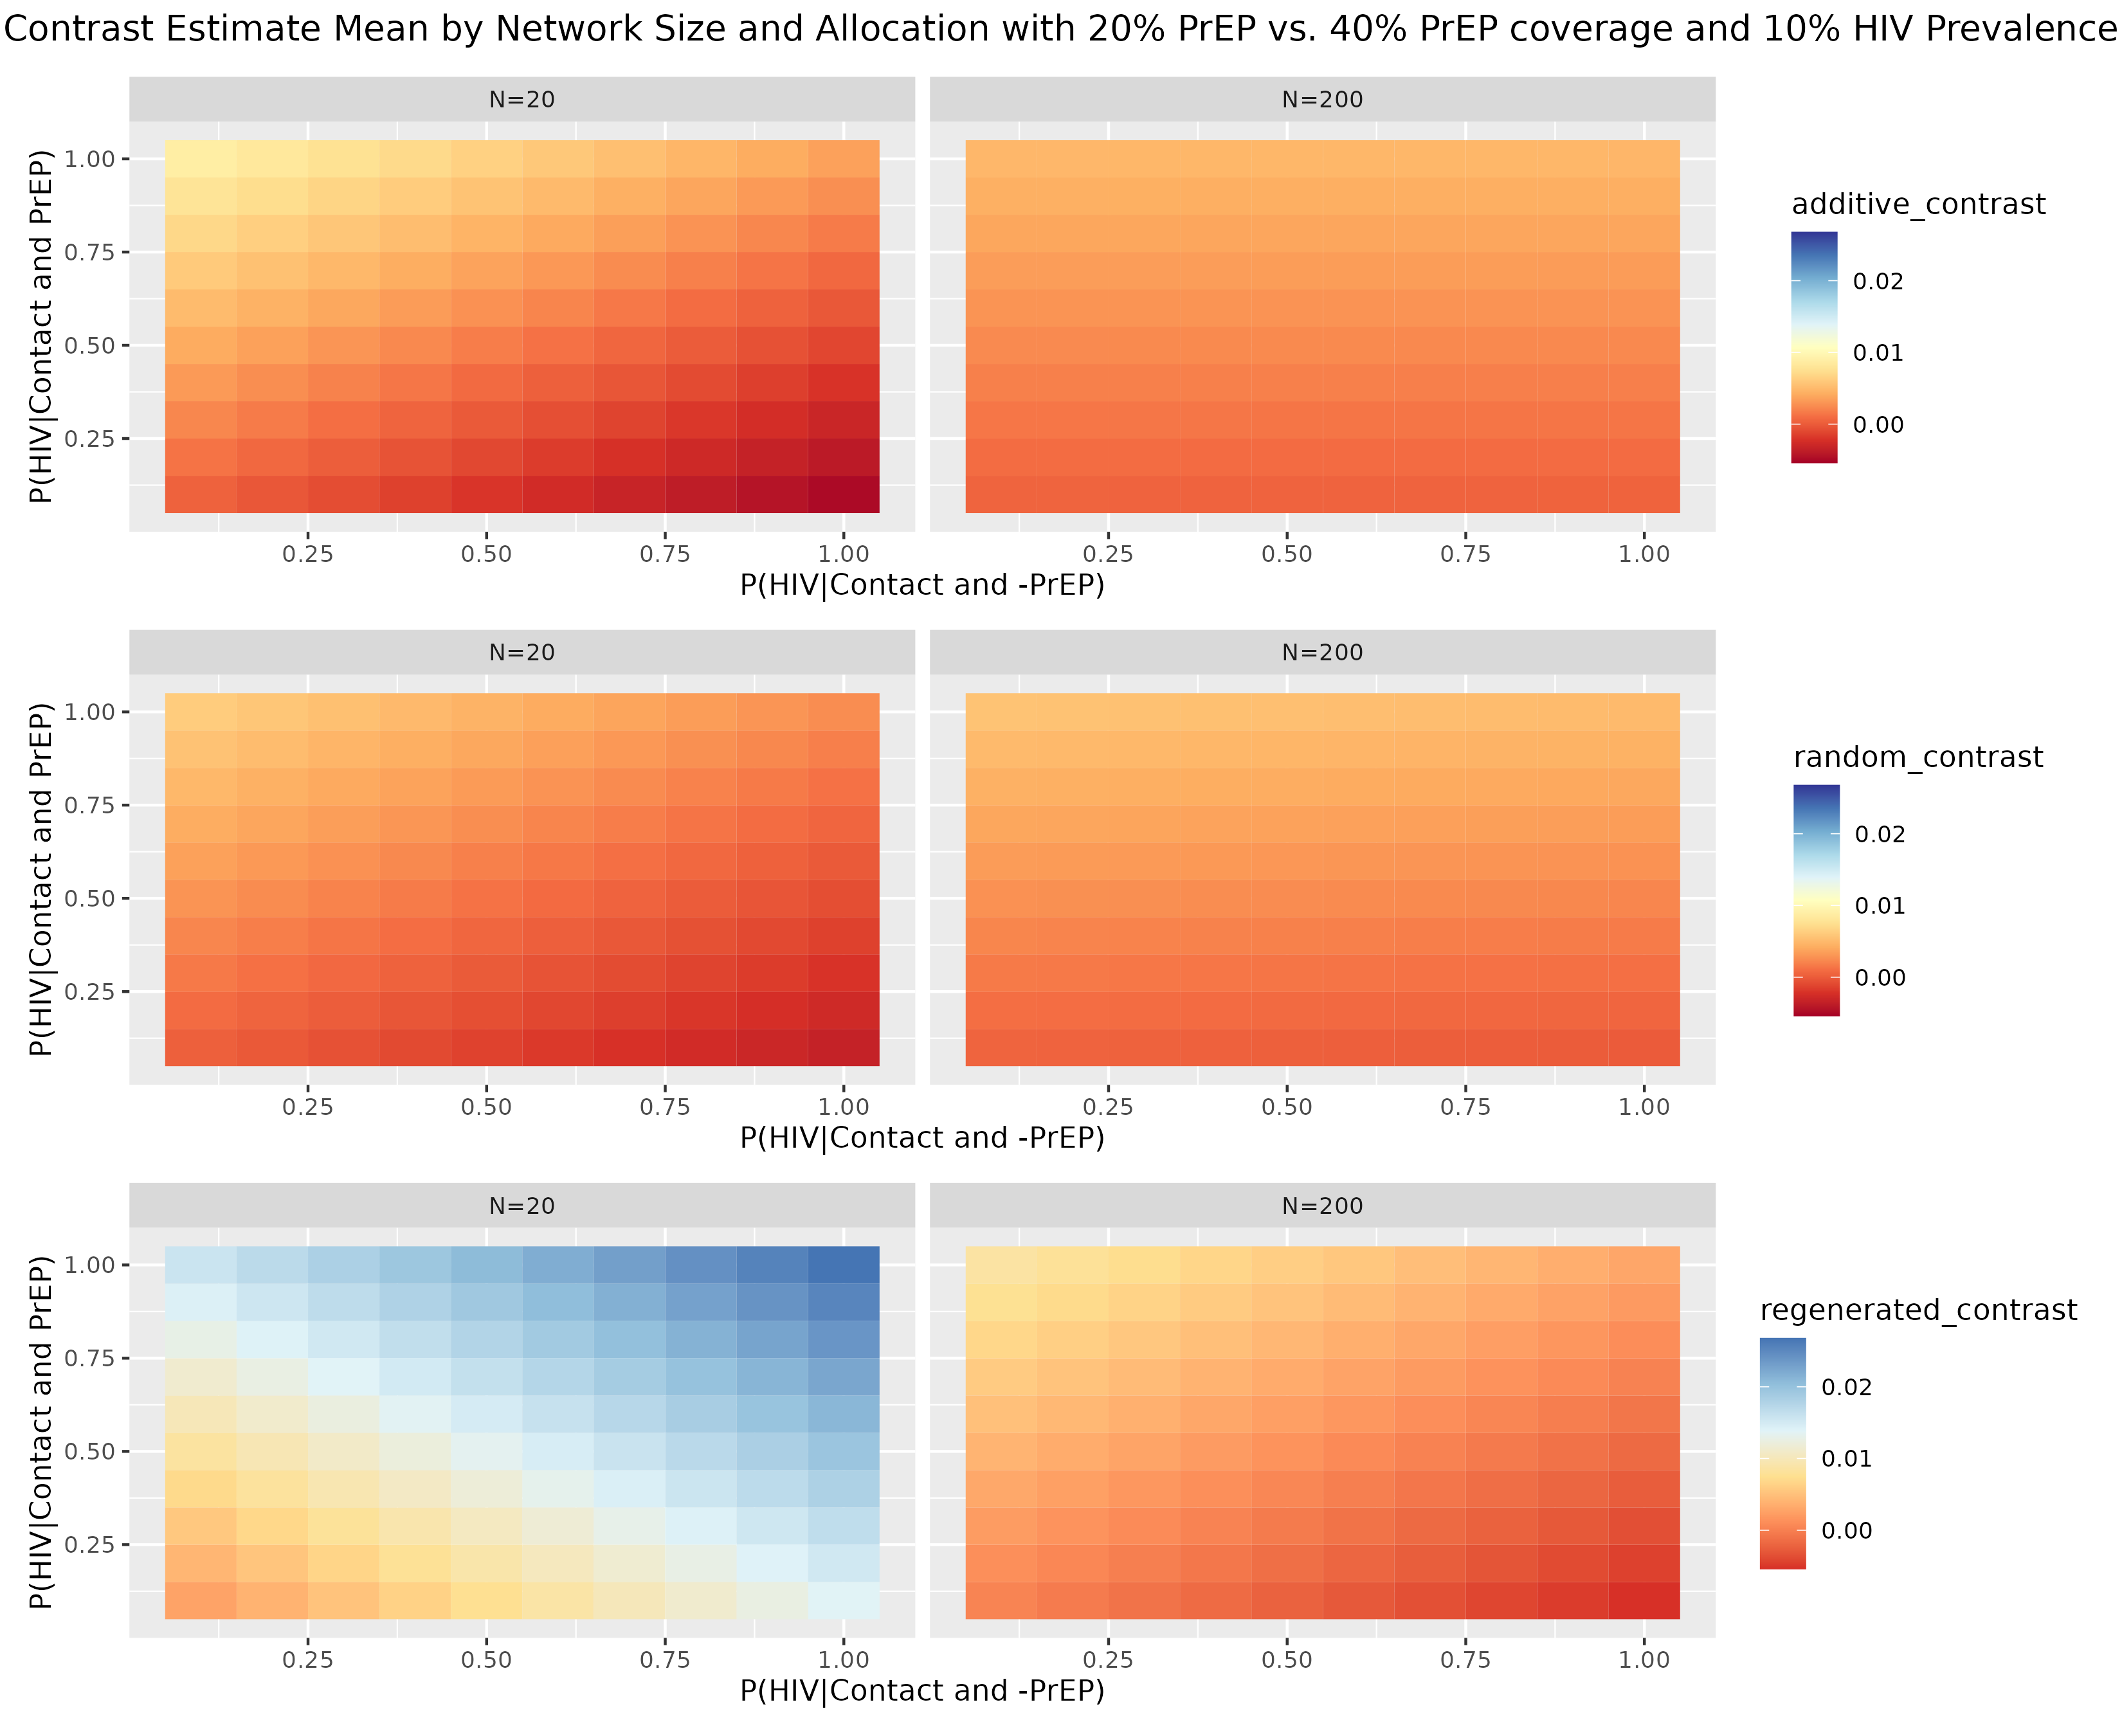
\includegraphics[width=\linewidth]{Corrected Figures/Network Size Mean Plot.png}
    \caption{Mean Causal Contrast estimates as $\mathbb{P}\left[\text{HIV} \vert \neg \text{PrEP} \cap \text{Contact}\right]$ and $\mathbb{P}\left[\text{HIV} \vert \text{PrEP} \cap \text{Contact}\right]$ increase, stratified by Network Size/Graph Order. From top to bottom: ``additive" Mean Contrast of random 20\% additional vs. random 20\% PrEP allocation control, ``random" Mean Contrast of random 40\% PrEP allocation vs. random 20\% control, ``regenerated" Mean Contrast of random 40\% allocation on regenerated network vs. random 20\% control. }
    \label{fig: Figure S4.1}
\end{figure}
\begin{figure}[H]
    \centering
    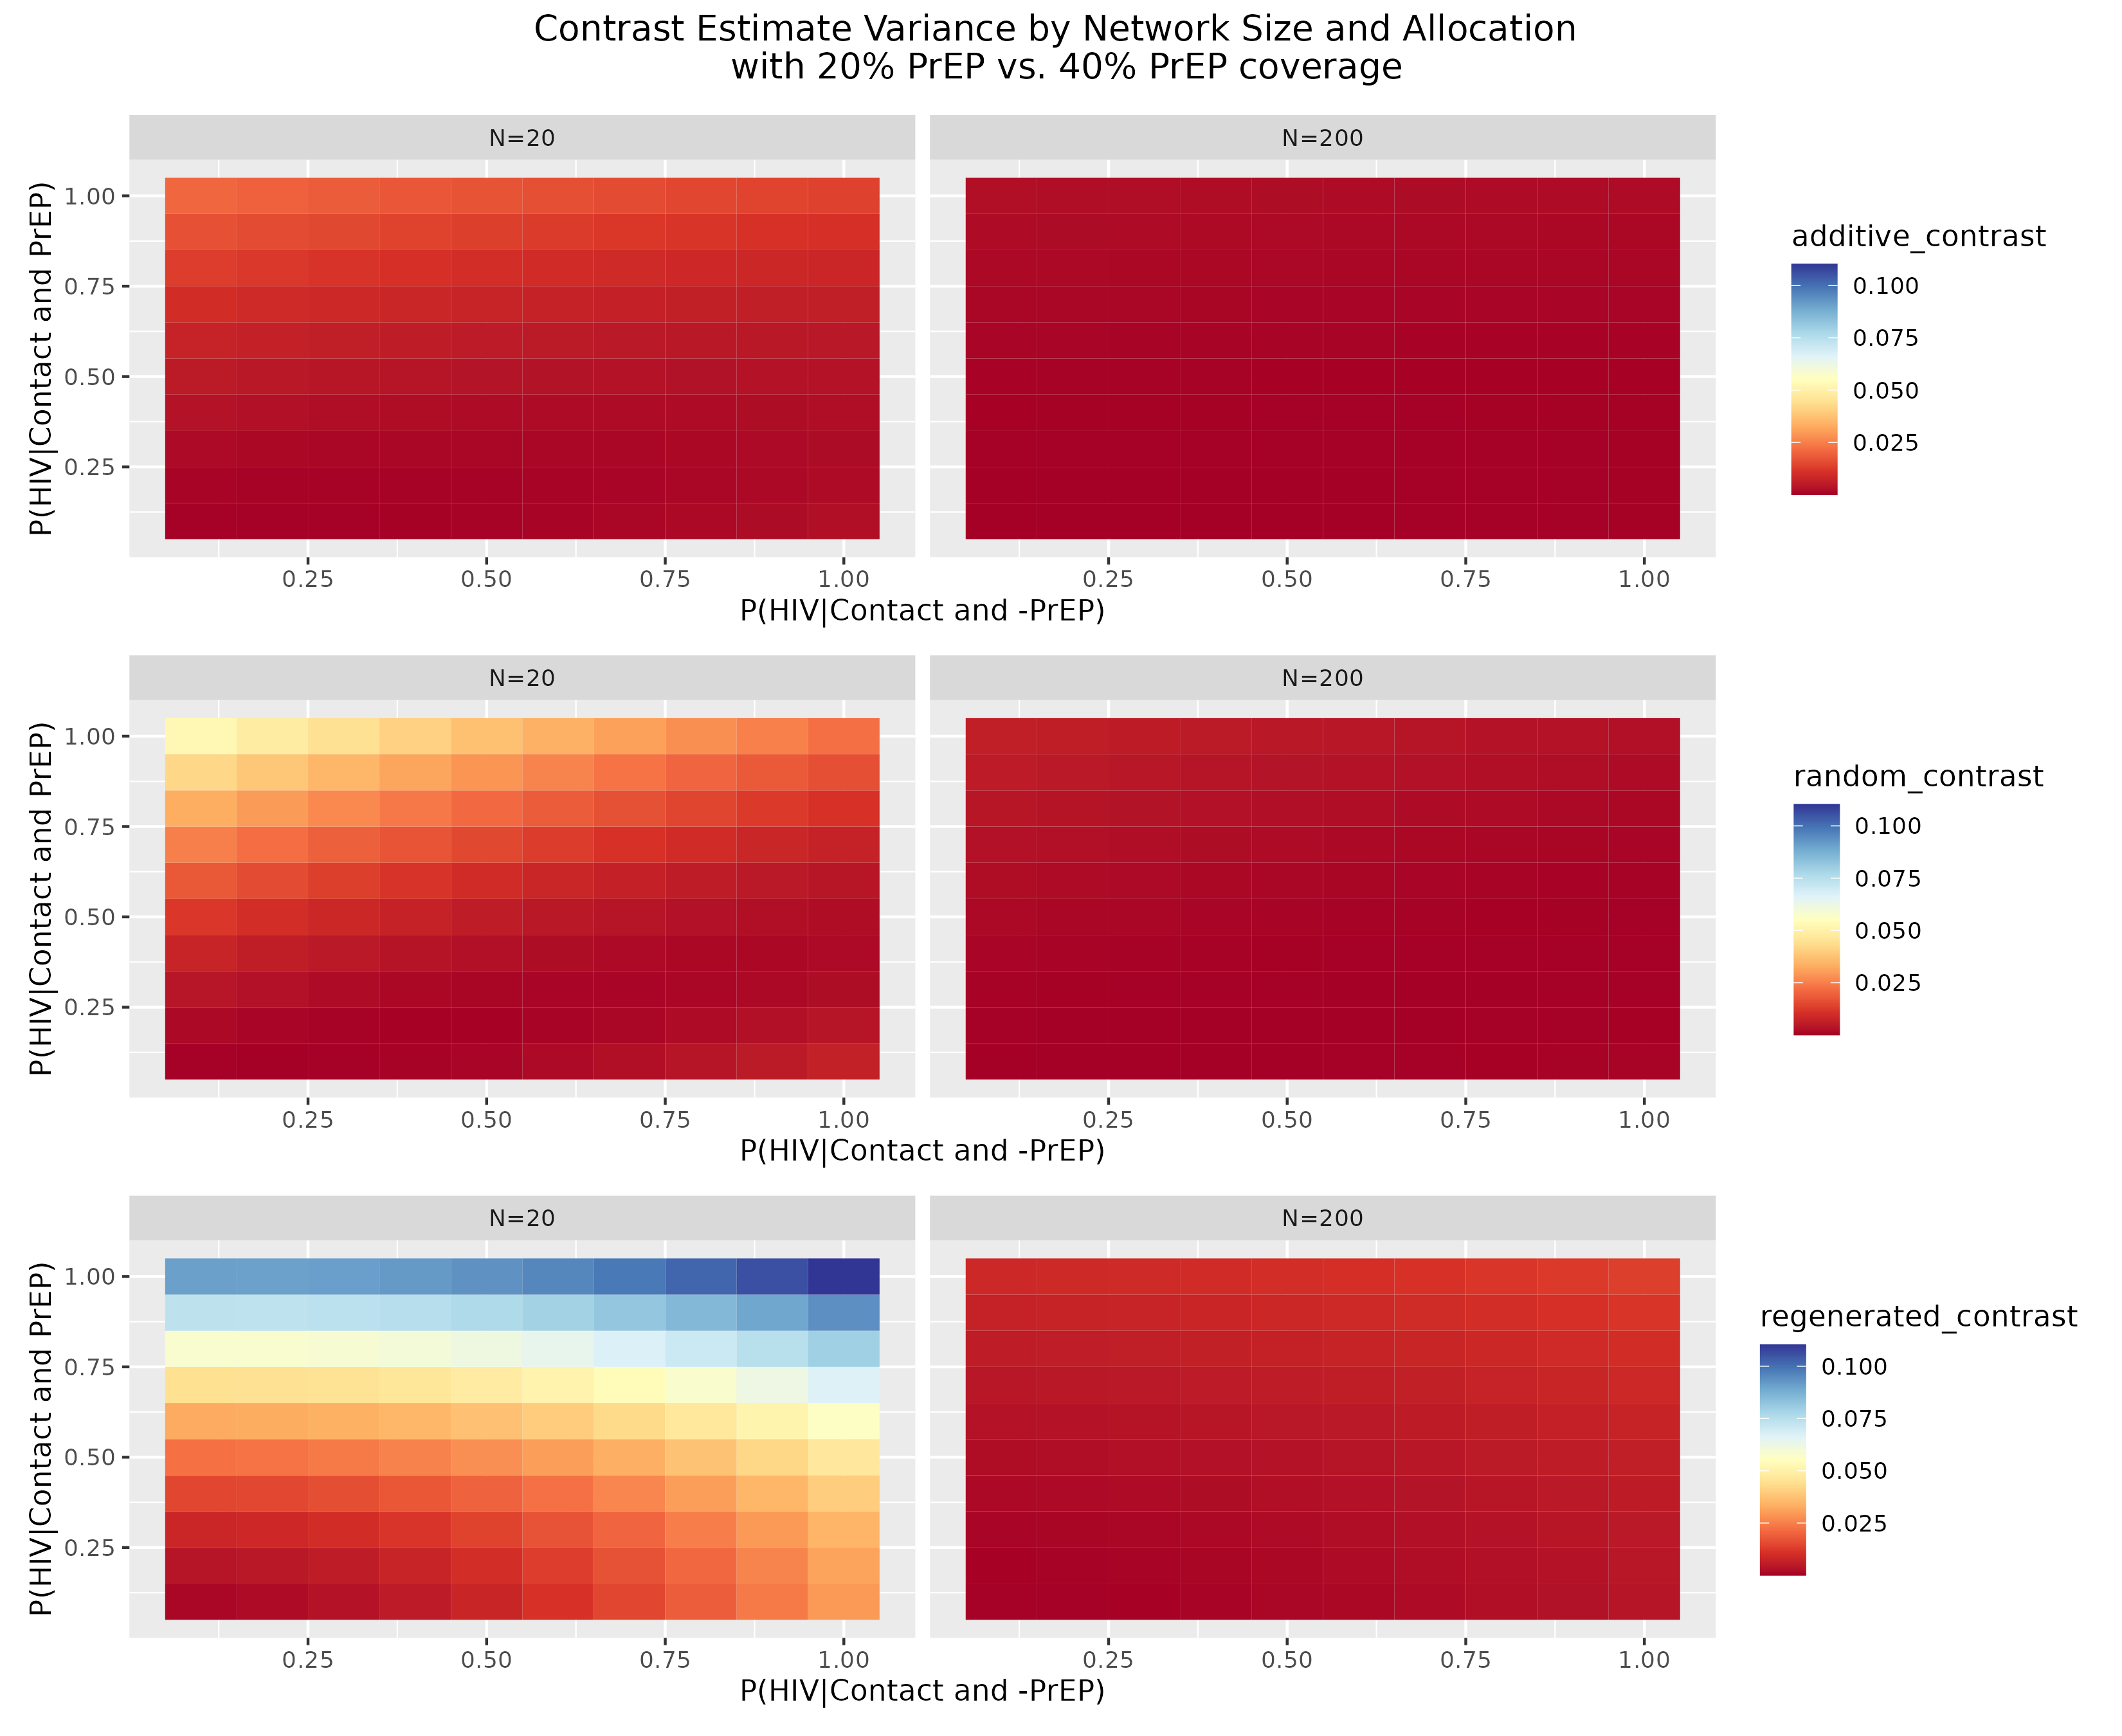
\includegraphics[width=\linewidth]{Corrected Figures/Network Size Variance plots.png}
    \caption{Variance of Causal Contrast estimates  as $\mathbb{P}\left[\text{HIV} \vert \neg \text{PrEP} \cap \text{Contact}\right]$ and $\mathbb{P}\left[\text{HIV} \vert \text{PrEP} \cap \text{Contact}\right]$ increase, stratified by Network Size/Graph Order. From top to bottom: ``additive" Variance of Contrast of random 20\% additional vs. random 20\% PrEP allocation control, ``random" Variance of Contrast of random 40\% PrEP allocation vs. random 20\% control, ``regenerated" Variance of Contrast of random 40\% allocation on regenerated network vs. random 20\% control.}
    \label{fig:Figure S4.2}
\end{figure}
From both the Mean and Variance plots above, there is apparent effect modification of the relationship between ``risks" of HIV and treatment allocation strategy at small network sizes. However, this modification essentially disappears in (order of magnitude) larger networks. The effect modification is particularly apparent with respect to the regenerated networks where the means are most variable across risk combinations (as well as the variances themselves).  

\subsubsection{Effect Modification by Sample Size}
\begin{figure}[H]
    \centering
    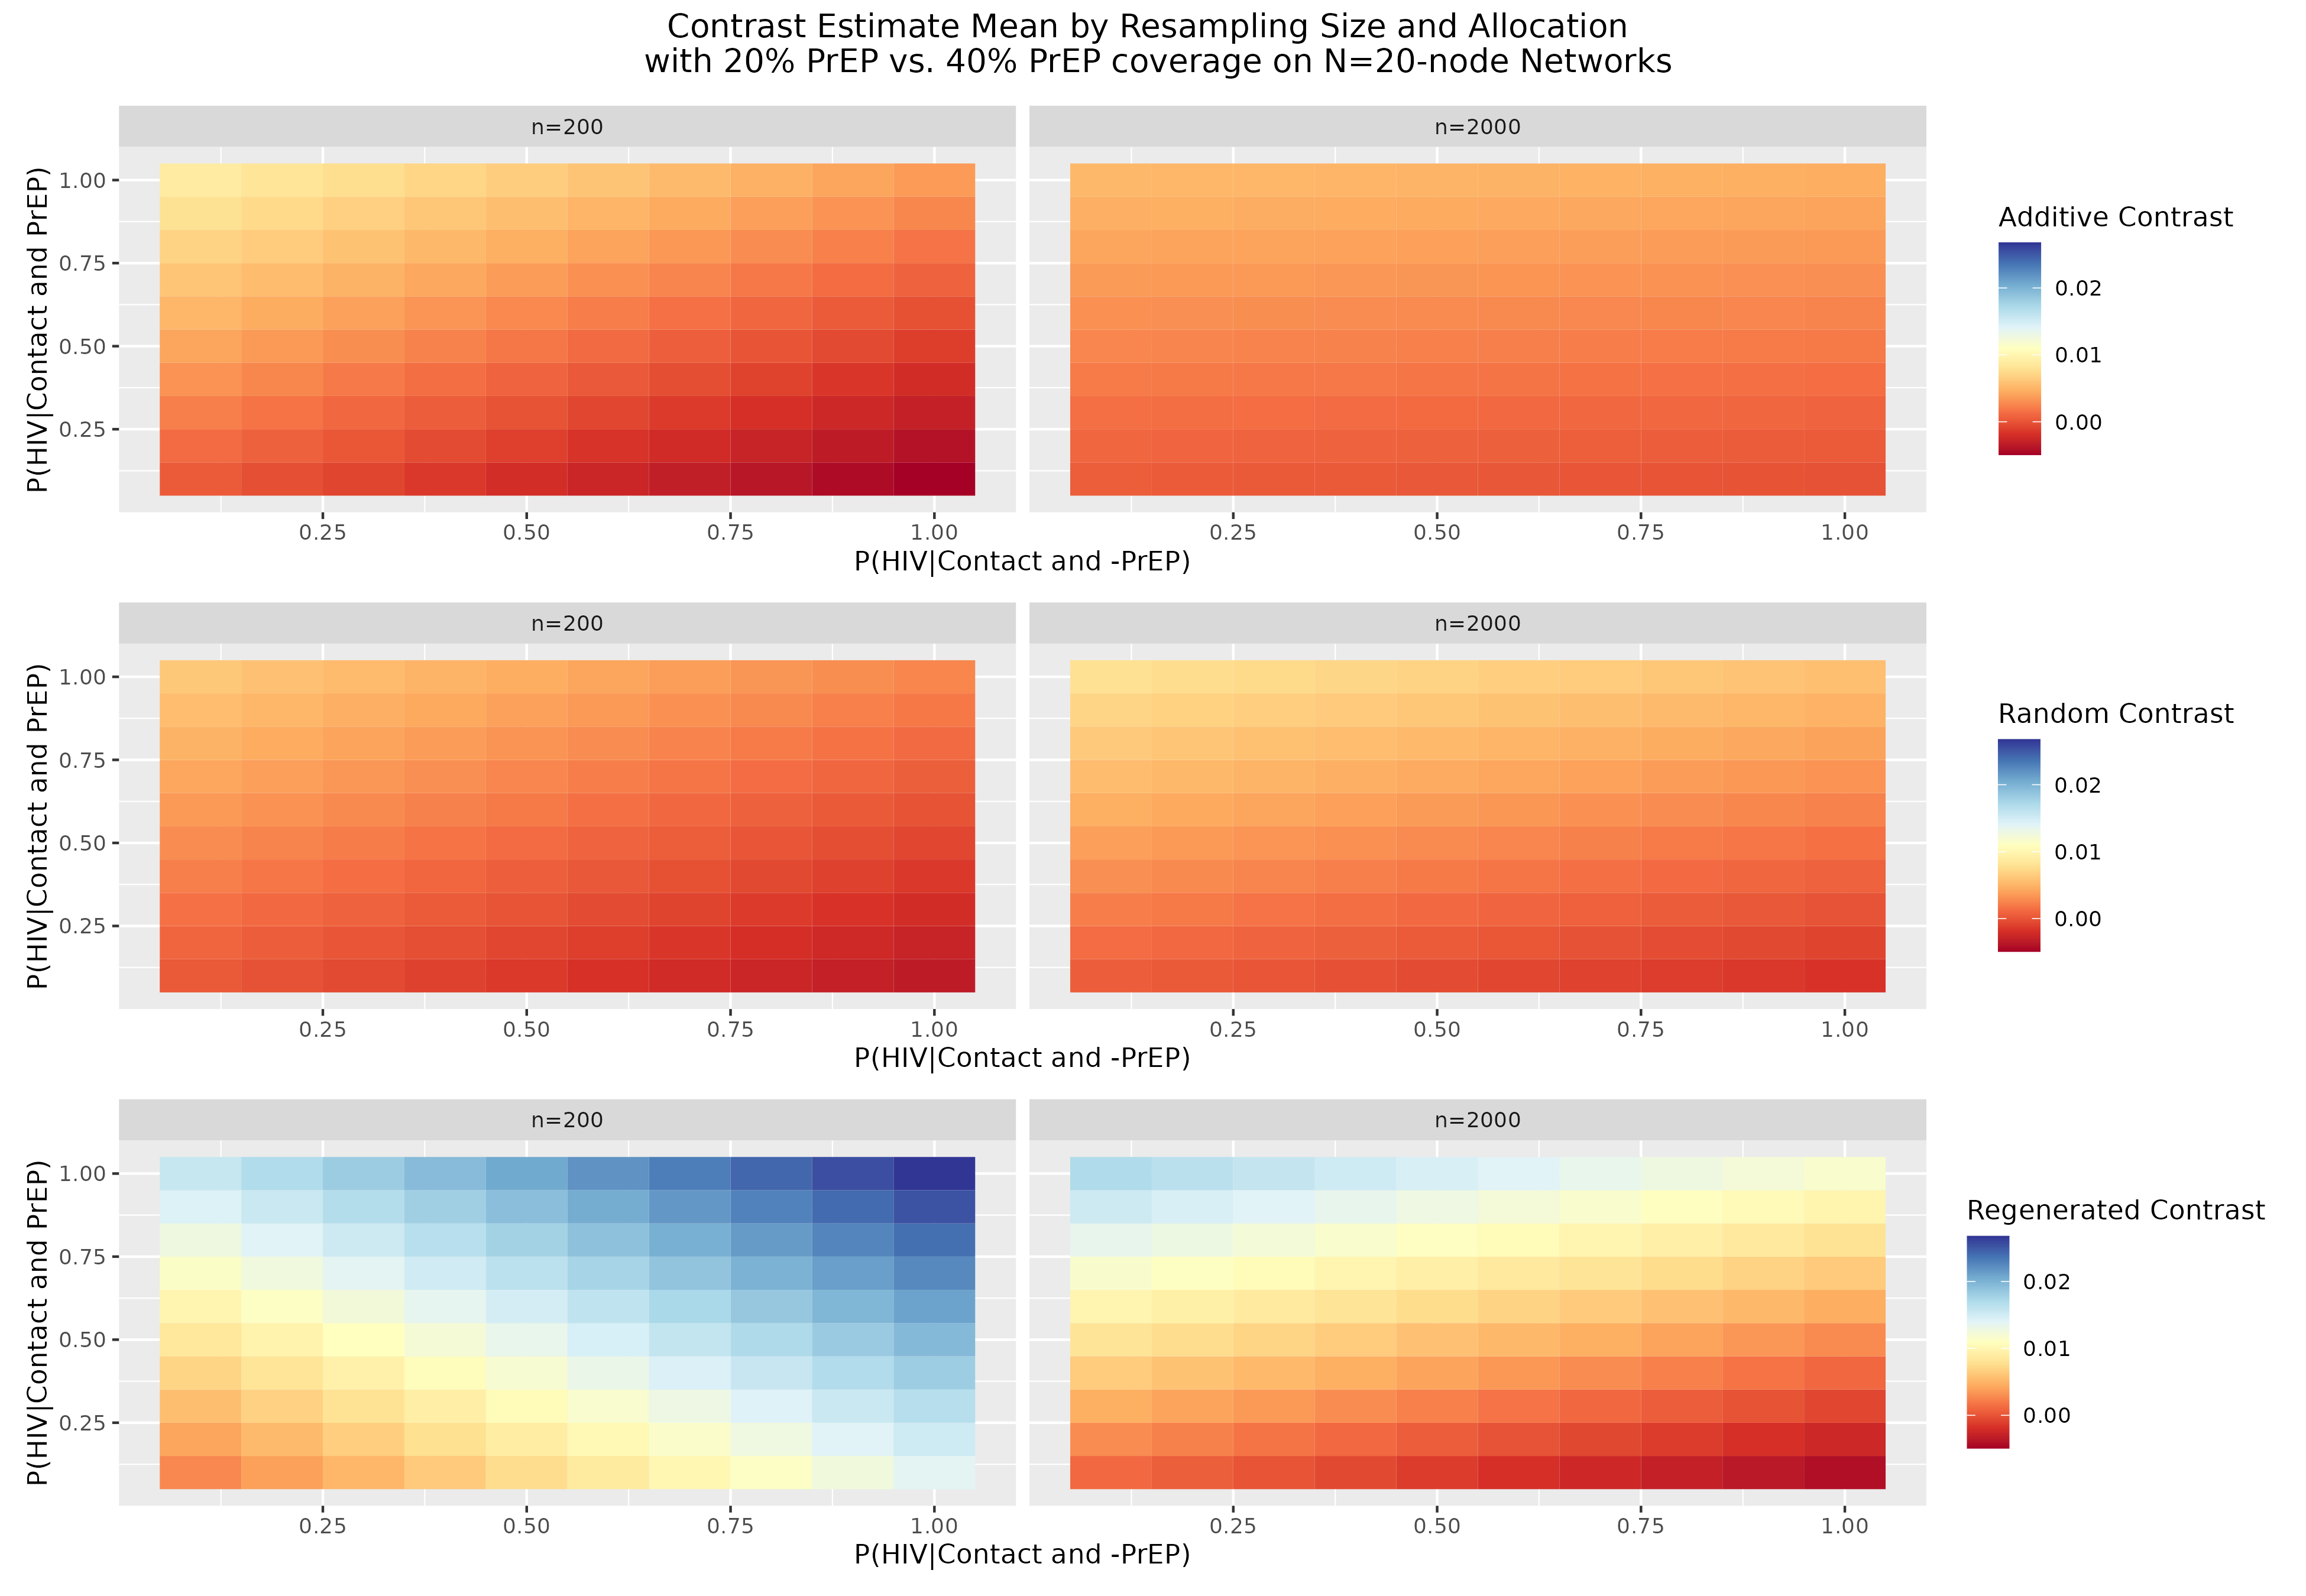
\includegraphics[width=\linewidth]{Corrected Figures/Resampling Size Mean Plot.png}
    \caption{Mean Causal Contrast estimates as $\mathbb{P}\left[\text{HIV} \vert \neg \text{PrEP} \cap \text{Contact}\right]$ and $\mathbb{P}\left[\text{HIV} \vert \text{PrEP} \cap \text{Contact}\right]$ increase, stratified by resampling sample size. From top to bottom: ``additive" Mean Contrast of random 20\% additional vs. random 20\% PrEP allocation control, ``random" Mean Contrast of random 40\% PrEP allocation vs. random 20\% control, ``regenerated" Mean Contrast of random 40\% allocation on regenerated network vs. random 20\% control.}
    \label{fig:Figure S4.3}
\end{figure}
\begin{figure}[H]
    \centering
    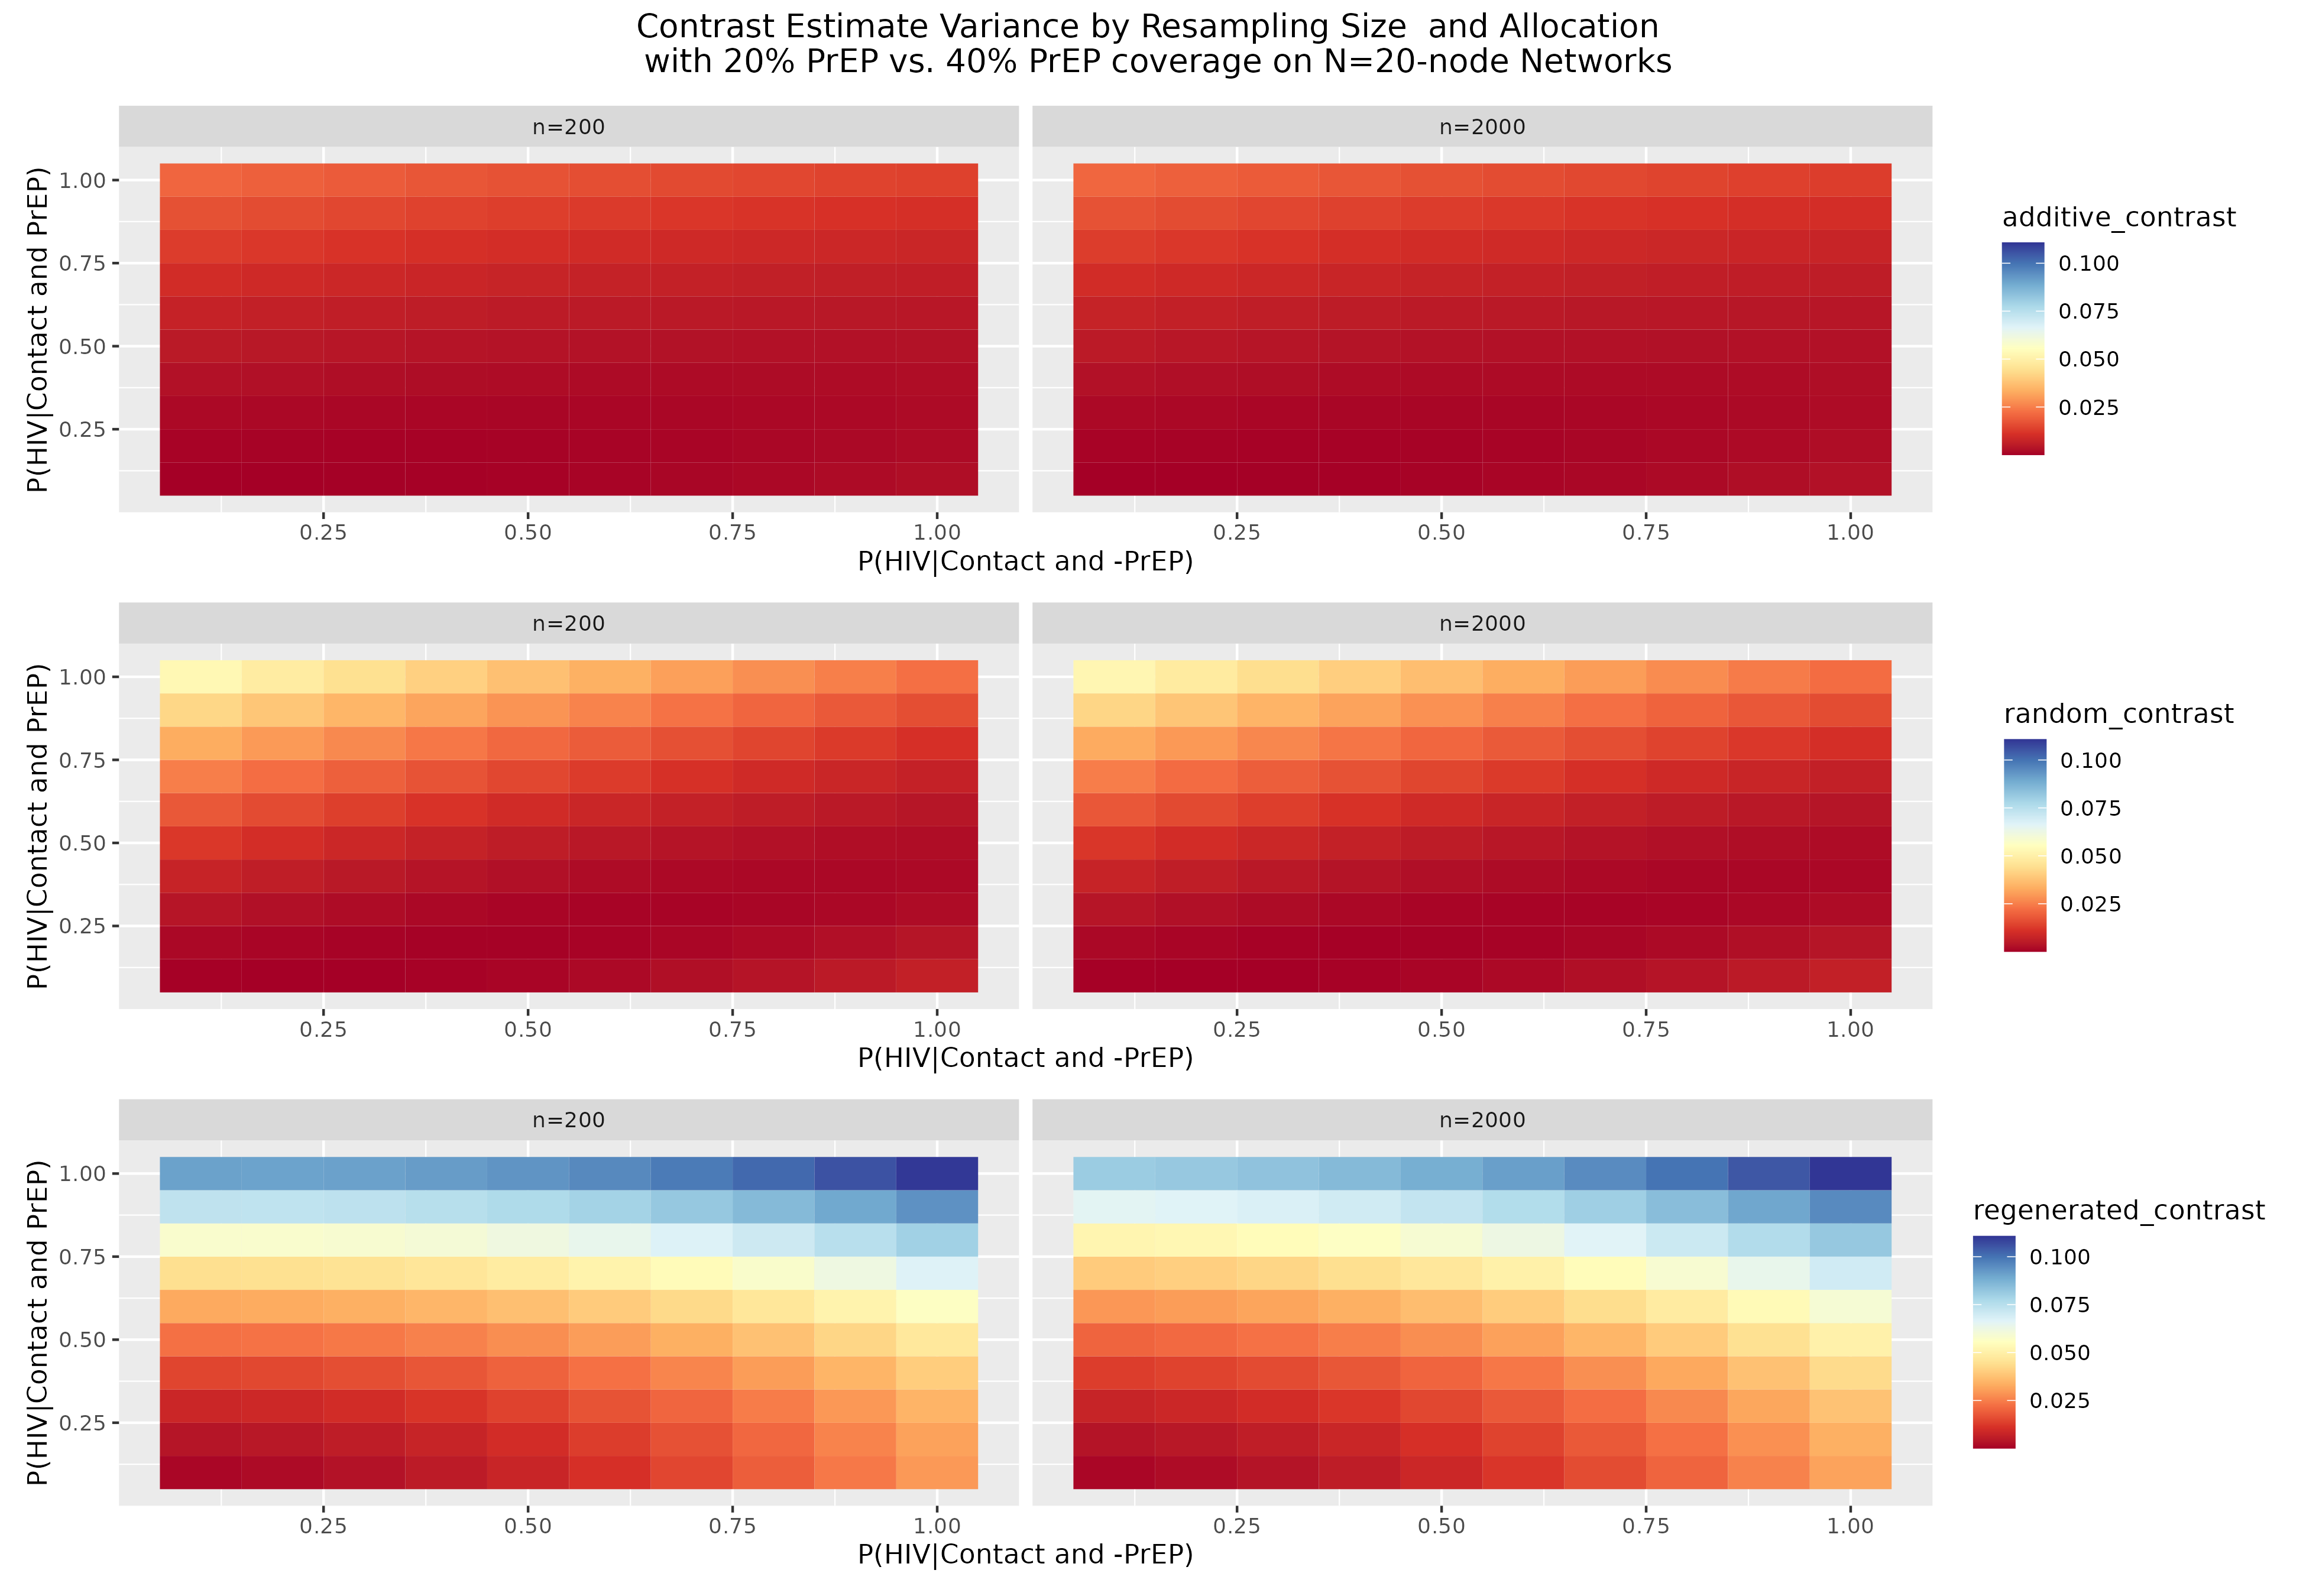
\includegraphics[width=\linewidth]{Corrected Figures/Resampling Size Variance Plot.png}
    \caption{Variance of Causal Contrast estimates as $\mathbb{P}\left[\text{HIV} \vert \neg \text{PrEP} \cap \text{Contact}\right]$ and $\mathbb{P}\left[\text{HIV} \vert \text{PrEP} \cap \text{Contact}\right]$ increase, stratified by resampling sample size. From top to bottom: ``additive" Variance of Contrast of random 20\% additional vs. random 20\% PrEP allocation control, ``random" Variance of Contrast of random 40\% PrEP allocation vs. random 20\% control, ``regenerated" Variance of Contrast of random 40\% allocation on regenerated network vs. random 20\% control.}
    \label{ffig:Figure S4.4}
\end{figure}
Much like with network size, effect modification of the relationship between underlying HIV risks and treatment strategy by resampling size is apparent in both Mean and Variance plots above. We can see clearly from these plots that Contrast estimate variances differ not only in range of magnitudes, but also follow very different gradients under different treatment strategies.
\subsubsection{Effect Modification by HIV Prevalence}
\begin{figure}[H]
    \centering
    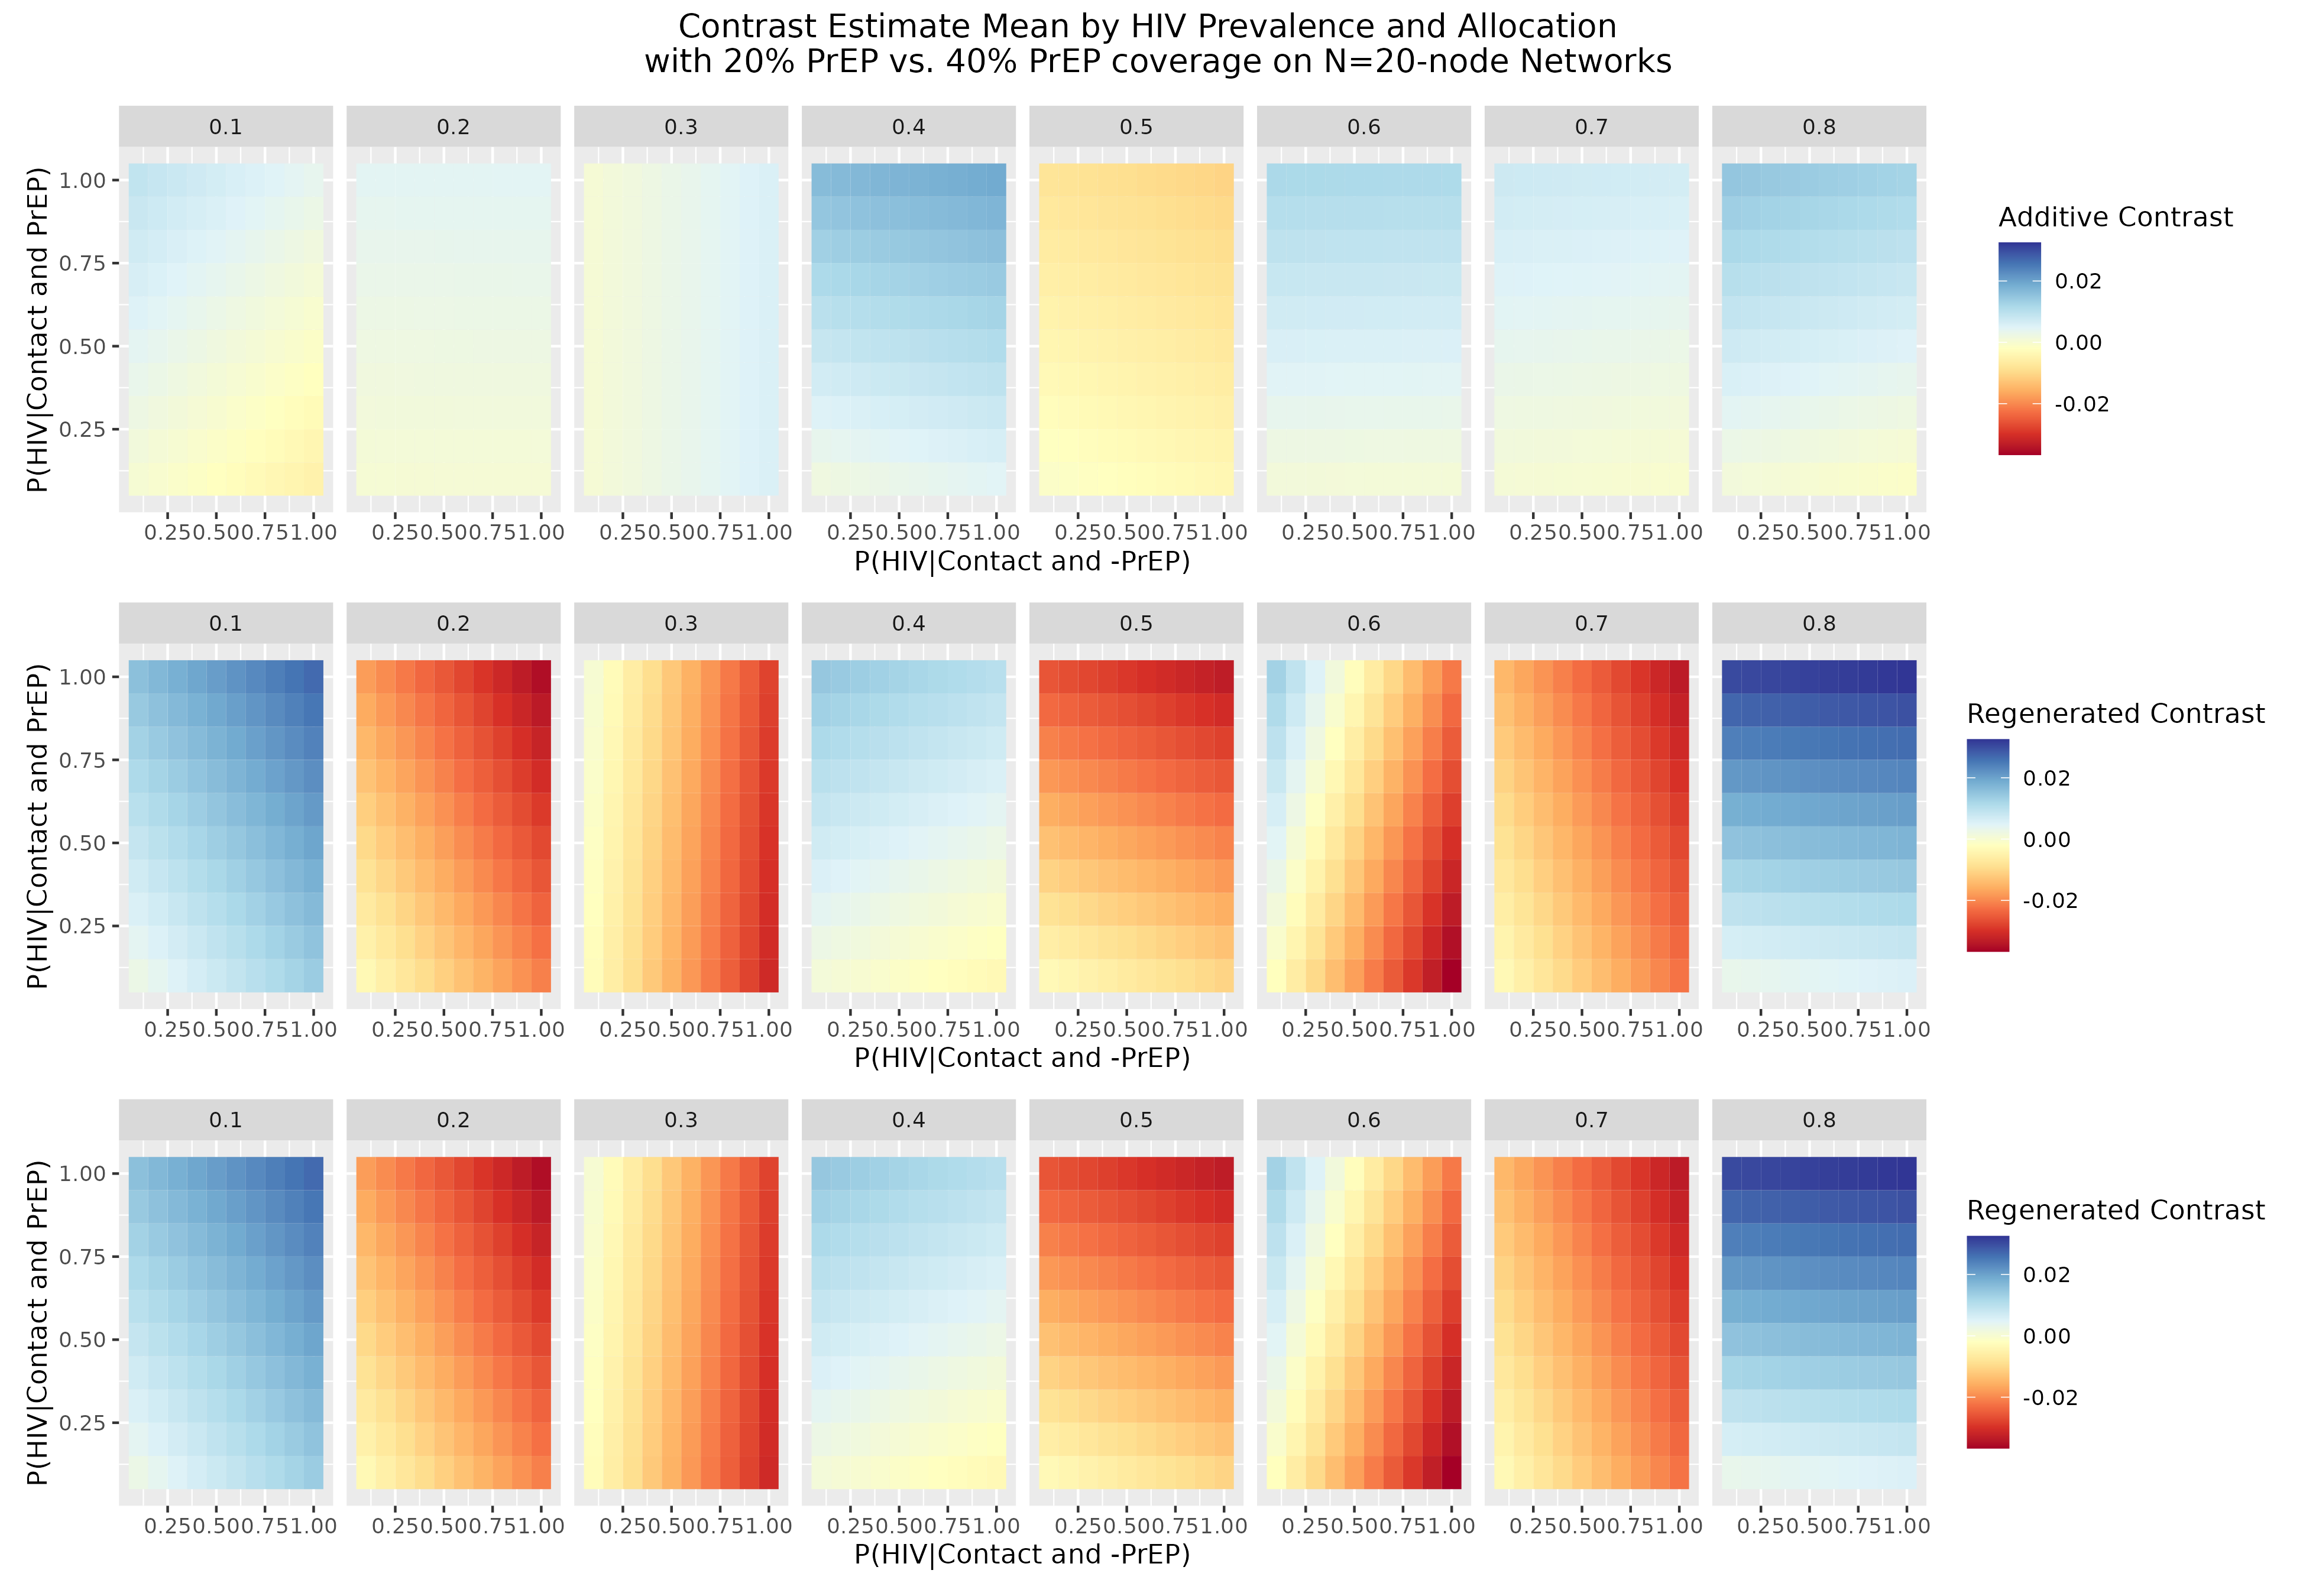
\includegraphics[width=\linewidth]{Corrected Figures/HIV Prevalence Mean Plot.png }
    \caption{Mean Causal Contrast estimates as $\mathbb{P}\left[\text{HIV} \vert \neg \text{PrEP} \cap \text{Contact}\right]$ and $\mathbb{P}\left[\text{HIV} \vert \text{PrEP} \cap \text{Contact}\right]$ increase,  stratified by HIV Prevalence. From top to bottom: ``additive" Mean Contrast of random 20\% additional vs. random 20\% PrEP allocation control, ``random" Mean Contrast of random 40\% PrEP allocation vs. random 20\% control, ``regenerated" Mean Contrast of random 40\% allocation on regenerated network vs. random 20\% control.}
    \label{fig:Figure S4.5}
\end{figure}
\begin{figure}[H]
    \centering
    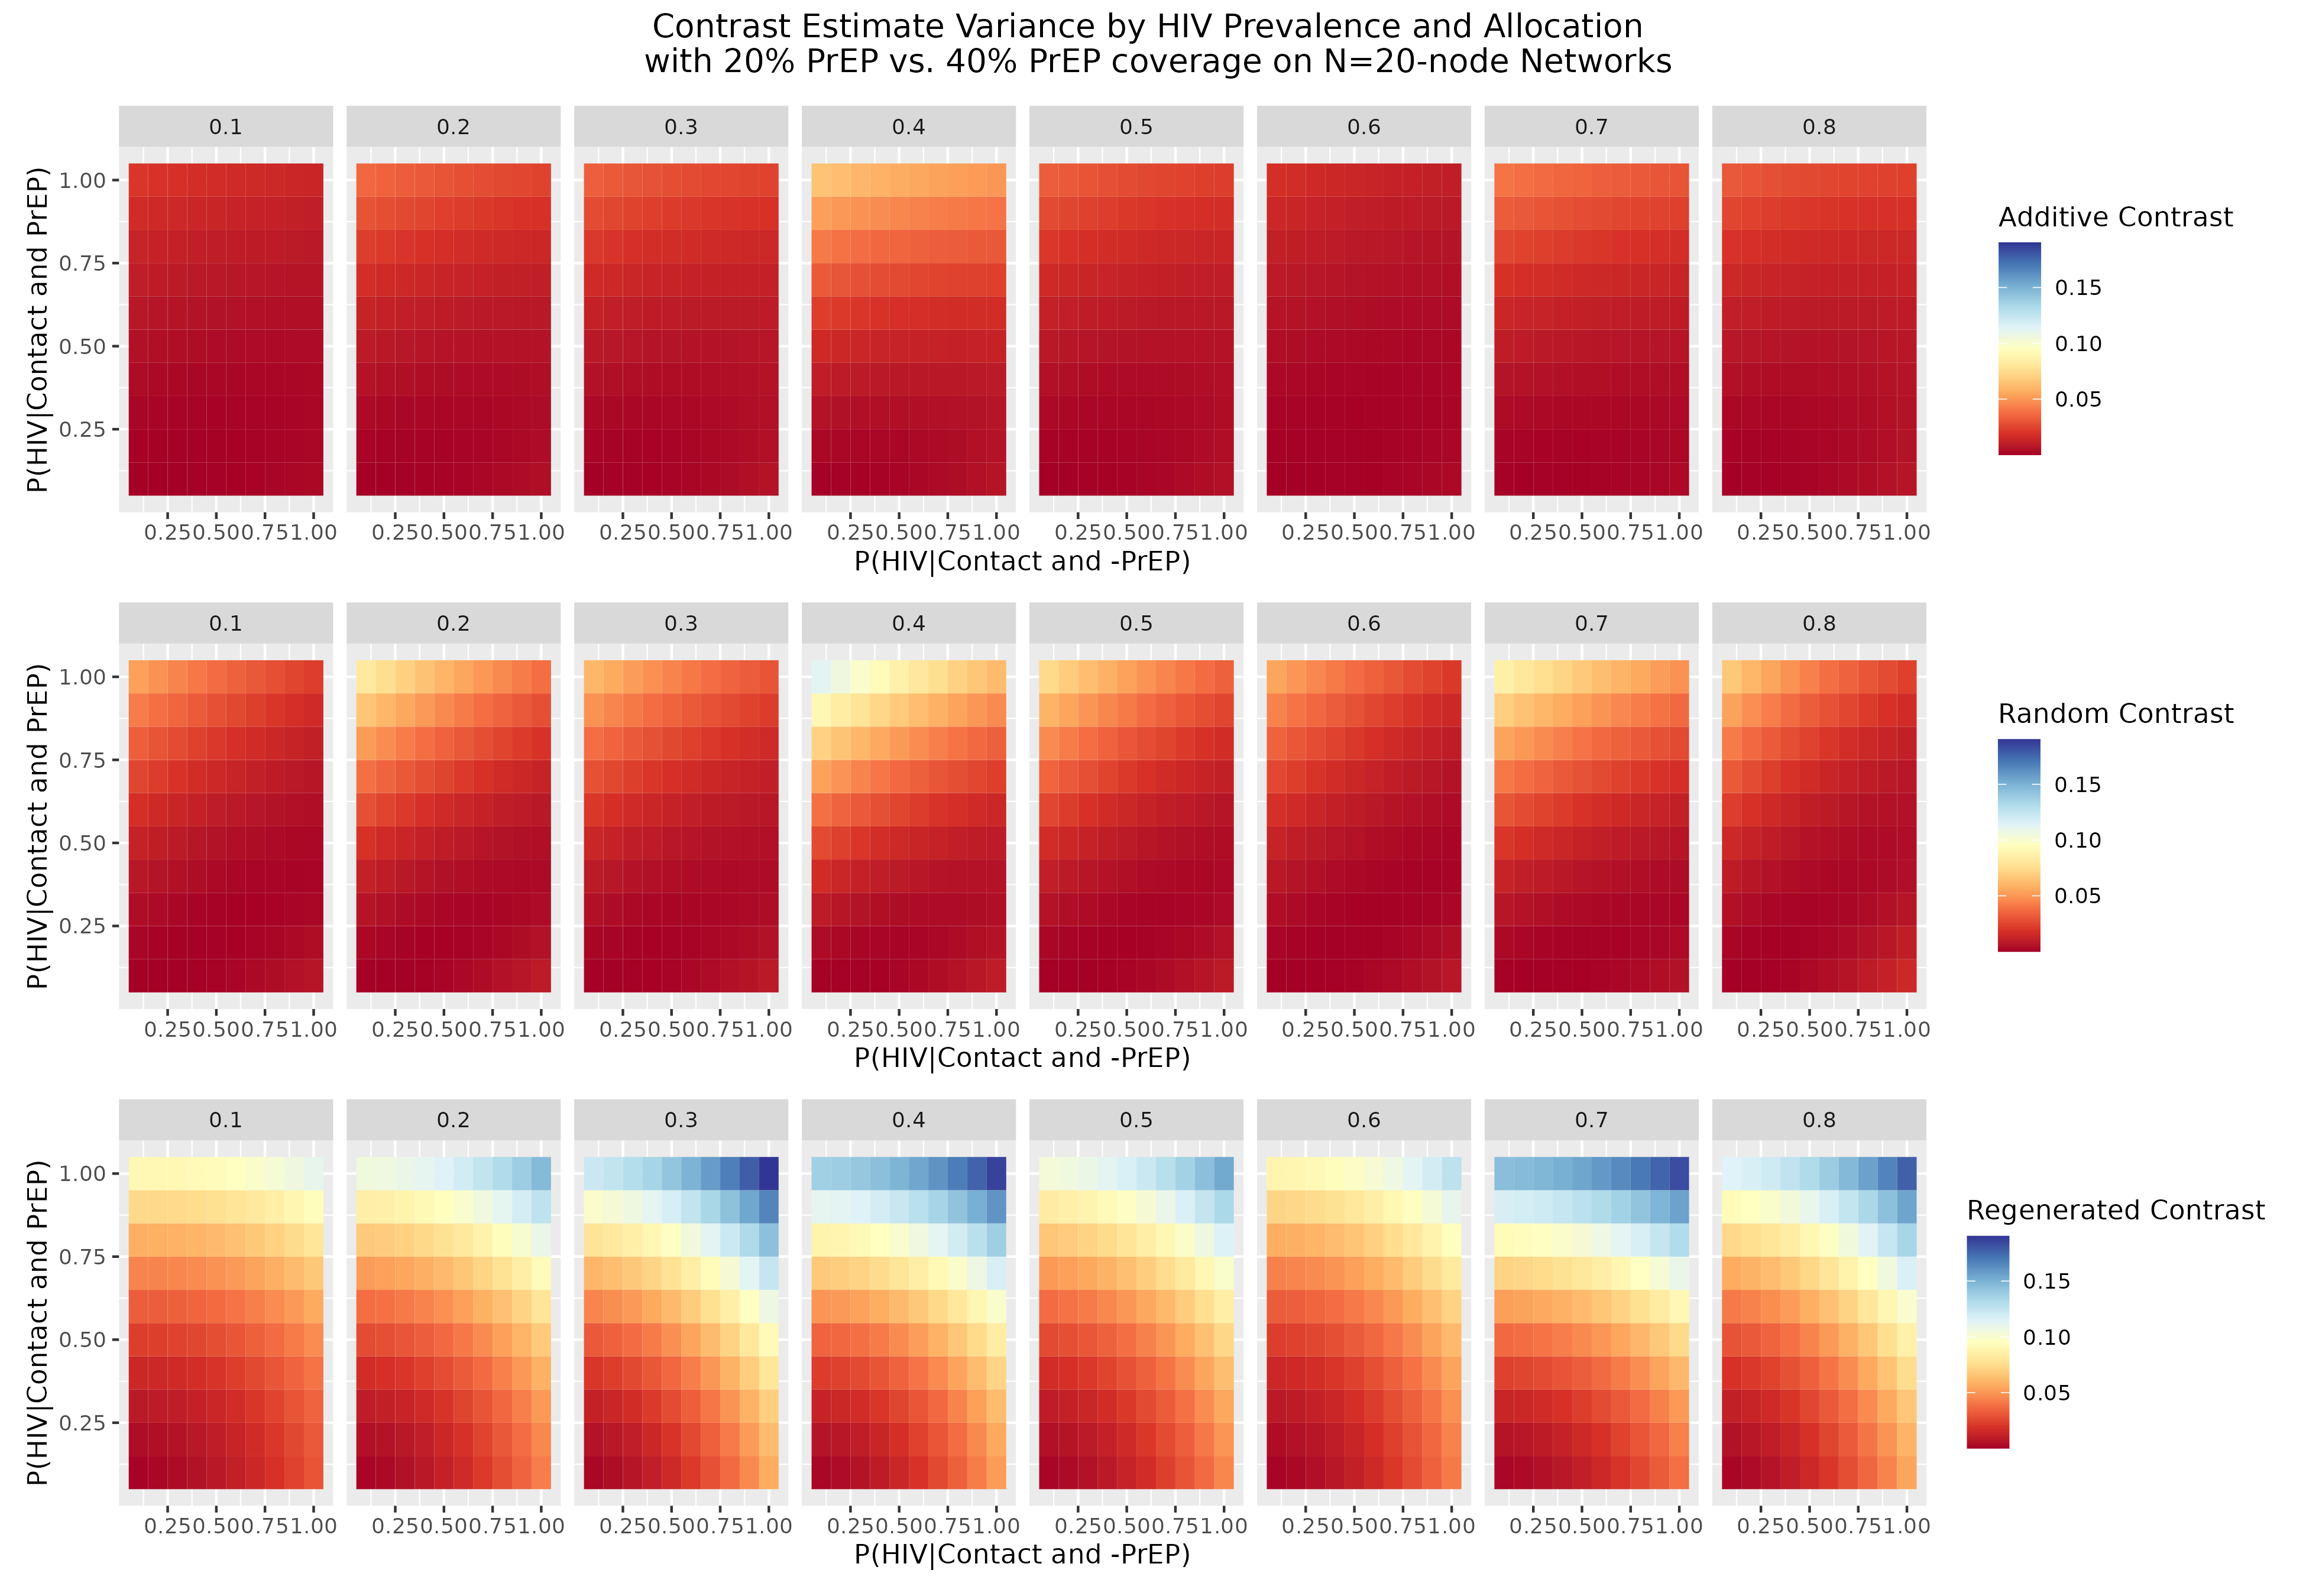
\includegraphics[width=\linewidth]{Corrected Figures/HIV Prevalence Variance Plot.png}
    \caption{Variance of Causal Contrast estimates as $\mathbb{P}\left[\text{HIV} \vert \neg \text{PrEP} \cap \text{Contact}\right]$ and $\mathbb{P}\left[\text{HIV} \vert \text{PrEP} \cap \text{Contact}\right]$ increase,  stratified by HIV Prevalence. From top to bottom: ``additive" Variance of Contrast of random 20\% additional vs. random 20\% PrEP allocation control, ``random" Variance of Contrast of random 40\% PrEP allocation vs. random 20\% control, ``regenerated" Variance of Contrast of random 40\% allocation on regenerated network vs. random 20\% control.}
    \label{fig:Figure S4.6}
\end{figure}

While it may be more obvious from the Variance plots in Figure \ref{fig:Figure S4.6} than in the Mean plots \ref{fig:Figure S4.5}, there is apparent effect modification of the relationship between underlying HIV risks and treatment strategy by the initial HIV prevalence. We can see three distinct gradients in the magnitude of the contrast estimate Variance over the HIV risks for each of the treatment strategies, with distinct changes in these gradients by HIV prevalence. 
\subsubsection{Effect Modification by \texorpdfstring{$\mathbb{P}[\text{HIV } | \text {Contact } \cap \neg \text{ PrEP}]$}{ℙ[HIV | ¬PrEP]}}
\begin{figure}[H]
    \centering
    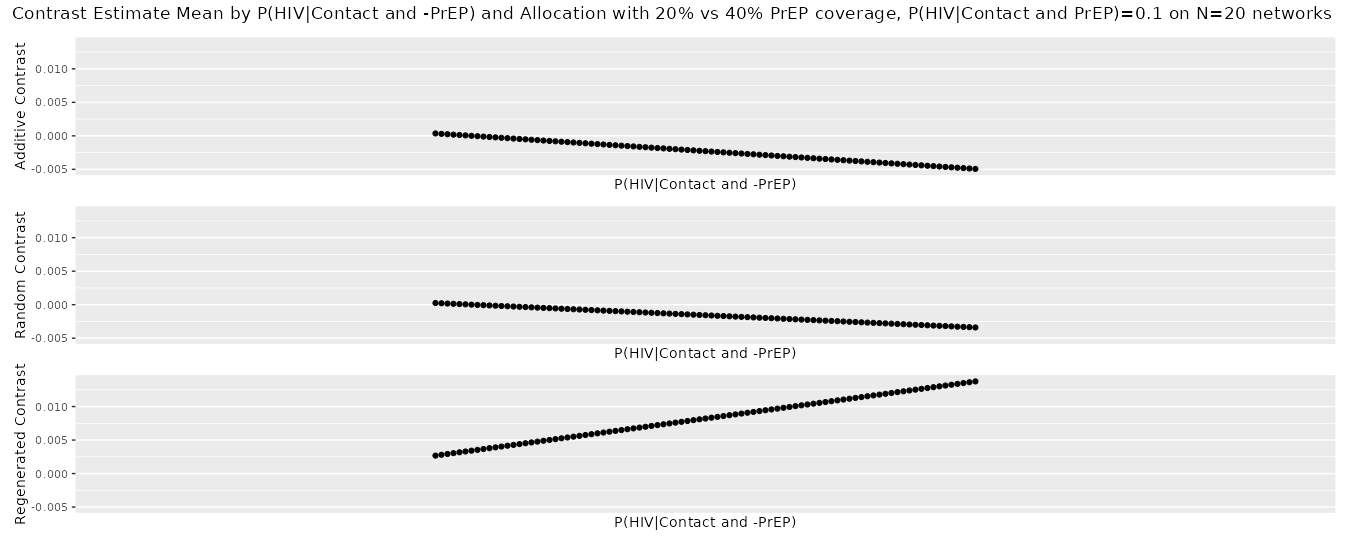
\includegraphics[width=\linewidth]{Corrected Figures/p1 Mean plots.png}
    \caption{Mean Causal Contrast estimates as $\mathbb{P}\left[\text{HIV } \vert \text {Contact } \cap \neg \text{ PrEP}\right]$ increases . From top to bottom: ``additive" Mean Contrast of random 20\% additional vs. random 20\% PrEP allocation control, ``random" Mean Contrast of random 40\% PrEP allocation vs. random 20\% control, ``regenerated" Mean Contrast of random 40\% allocation on regenerated network vs. random 20\% control.}
    \label{fig:Figure S4.7}
\end{figure}
\begin{figure}[H]
    \centering
    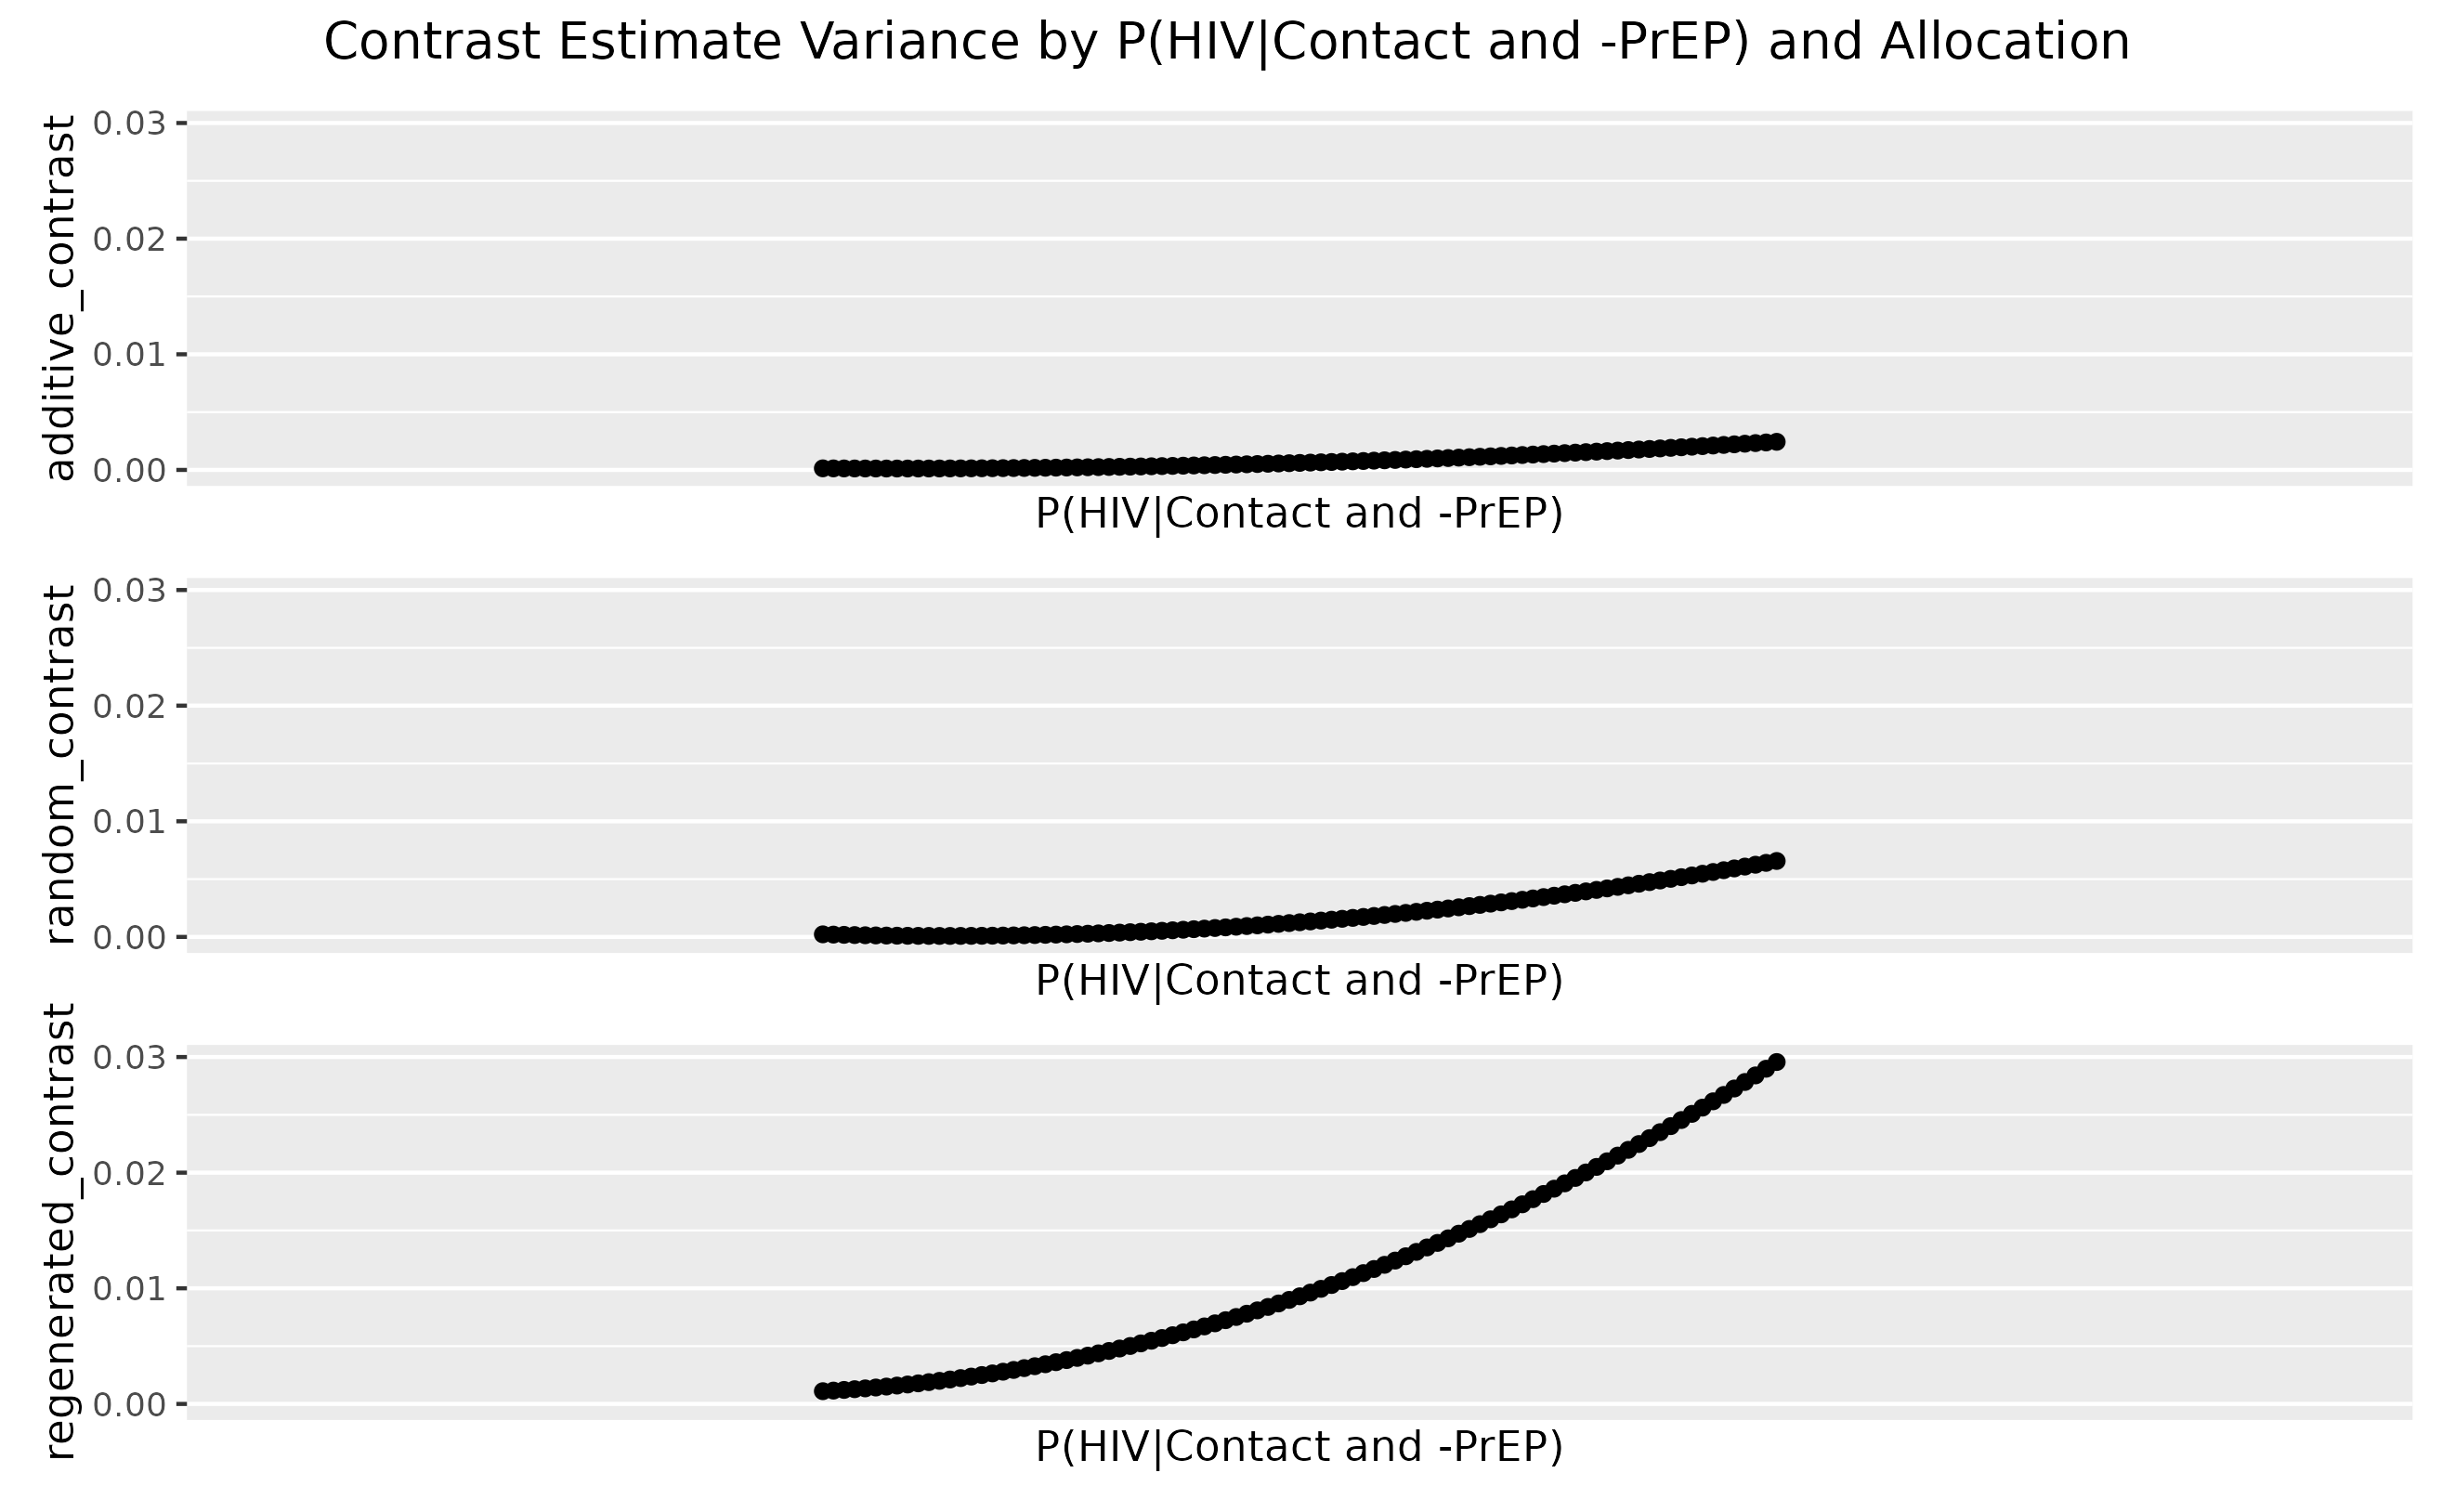
\includegraphics[width=\linewidth]{Corrected Figures/p1 Variance plots.png}
    \caption{Variance of Causal Contrast estimates as $\mathbb{P}\left[\text{HIV } \vert \text {Contact } \cap \neg \text{ PrEP}\right]$ increases .  From top to bottom: ``additive" Variance of Contrast of random 20\% additional vs. random 20\% PrEP allocation control, ``random" Variance of Contrast of random 40\% PrEP allocation vs. random 20\% control, ``regenerated" Variance of Contrast of random 40\% allocation on regenerated network vs. random 20\% control.}
    \label{fig:Figure S4.8}
\end{figure}
From the contrast estimate Mean and Variance plots in figures \ref{fig:Figure S4.7} and \ref{fig:Figure S4.8} above, we observe effect modification of the relationship between the underlying risk of HIV given contact and no treatment and HIV risk by treatment strategy. Whilst in the ``additive" treatment strategy, the contrast estimate Mean and Variance are both very small and relatively constant except for relatively large values of $\mathbb{P}\left[\text{HIV } \vert \text {Contact } \cap \neg \text{ PrEP}\right]$. The ``random" and ``regenerated" treatment strategies show marked heteroskedasticity beginning with much smaller values of $\mathbb{P}\left[\text{HIV } \vert \text {Contact } \cap \neg \text{ PrEP}\right]$, with the "regenerated" strategy usually having larger variability than the ``random" strategy for the same value of $\mathbb{P}\left[\text{HIV } \vert \text {Contact } \cap \neg \text{ PrEP}\right]$.  
\subsubsection{Effect Modification by \texorpdfstring{$\mathbb{P}\left[\text{HIV } \vert \text {Contact } \cap \text{ PrEP}\right]$}{ℙ[HIV | PrEP]}}
\begin{figure}[H]
    \centering
    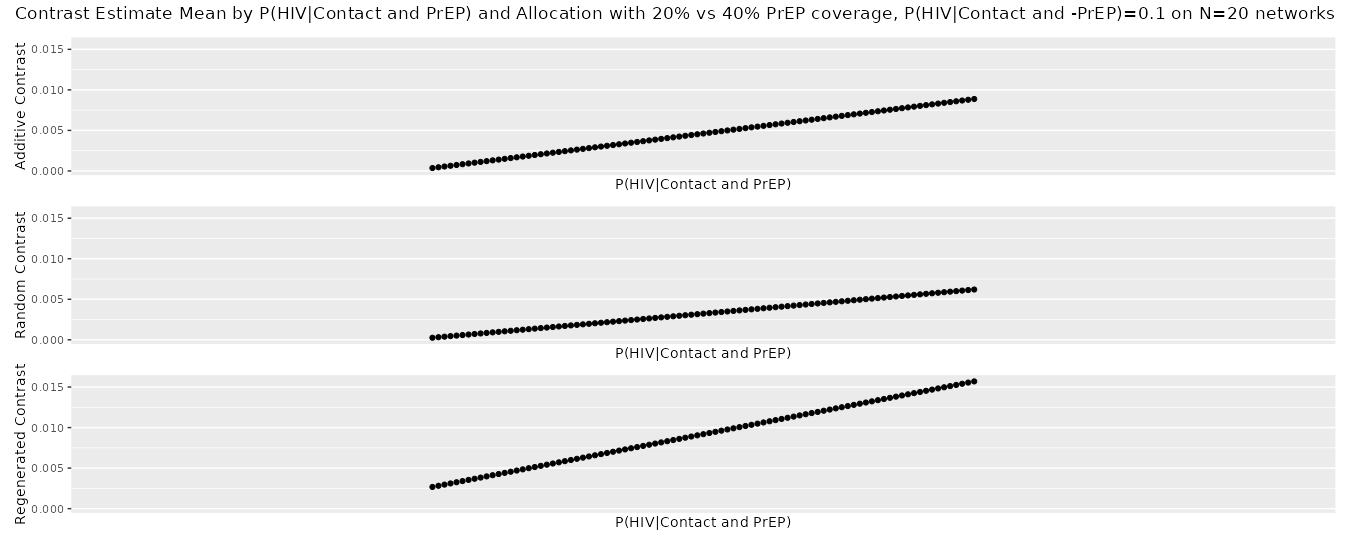
\includegraphics[width=\linewidth]{Corrected Figures/p2 Mean plots.png}
    \caption{Mean Causal Contrast estimates as $\mathbb{P}\left[\text{HIV } \vert \text{ PrEP}\right]$ increases . From top to bottom: ``additive" Mean Contrast of random 20\% additional vs. random 20\% PrEP allocation control, ``random" Mean Contrast of random 40\% PrEP allocation vs. random 20\% control, ``regenerated" Mean Contrast of random 40\% allocation on regenerated network vs. random 20\% control.}
    \label{fig:Figure S4.9}

\end{figure}

\begin{figure}[H]
    \centering
    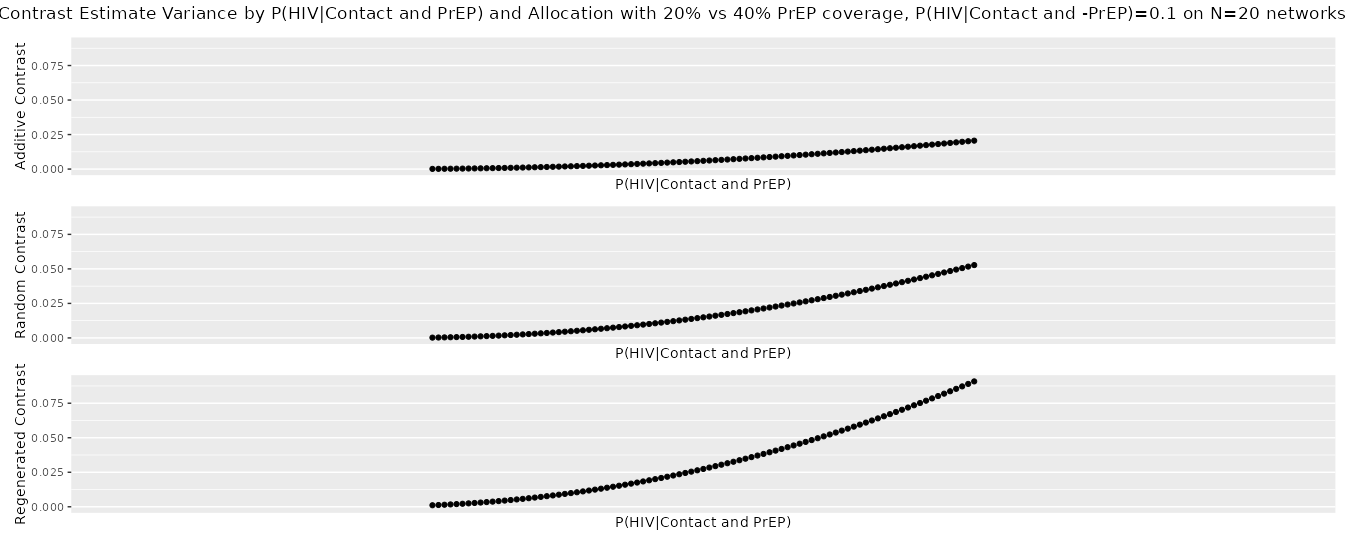
\includegraphics[width=\linewidth]{Corrected Figures/p2 Variance plots.png}
    \caption{Variance of Causal Contrast estimates as $\mathbb{P}\left[\text{HIV } \vert \text{ PrEP}\right]$ increases .  From top to bottom: ``additive" Variance of Contrast of random 20\% additional vs. random 20\% PrEP allocation control, ``random" Variance of Contrast of random 40\% PrEP allocation vs. random 20\% control, ``regenerated" Variance of Contrast of random 40\% allocation on regenerated network vs. random 20\% control.}
    \label{fig:Figure S4.10}
\end{figure}
Much like with the underlying risk of HIV given no treatment, we observe effect modification of the relationship between the underlying risk of HIV given infectious contact and PrEP treatment by allocation strategy. This modification is apparent in both Causal Contrast estimate Mean and Variance plots in Figure \ref{fig:Figure S4.9} and \ref{fig:Figure S4.10}, respectively. While the modification is qualitatively similar to that for the no treatment risk, it is interesting to note that the range of both Mean and Variance magnitudes is larger for $\mathbb{P}\left[\text{HIV } \vert \text{ PrEP}\right]$ than for $\mathbb{P}\left[\text{HIV } \vert \text {Contact } \cap \neg \text{ PrEP}\right]$.

\subsubsection{Effect Modification by PrEP contrasts in ER model}
\begin{figure}[H]
    \centering
    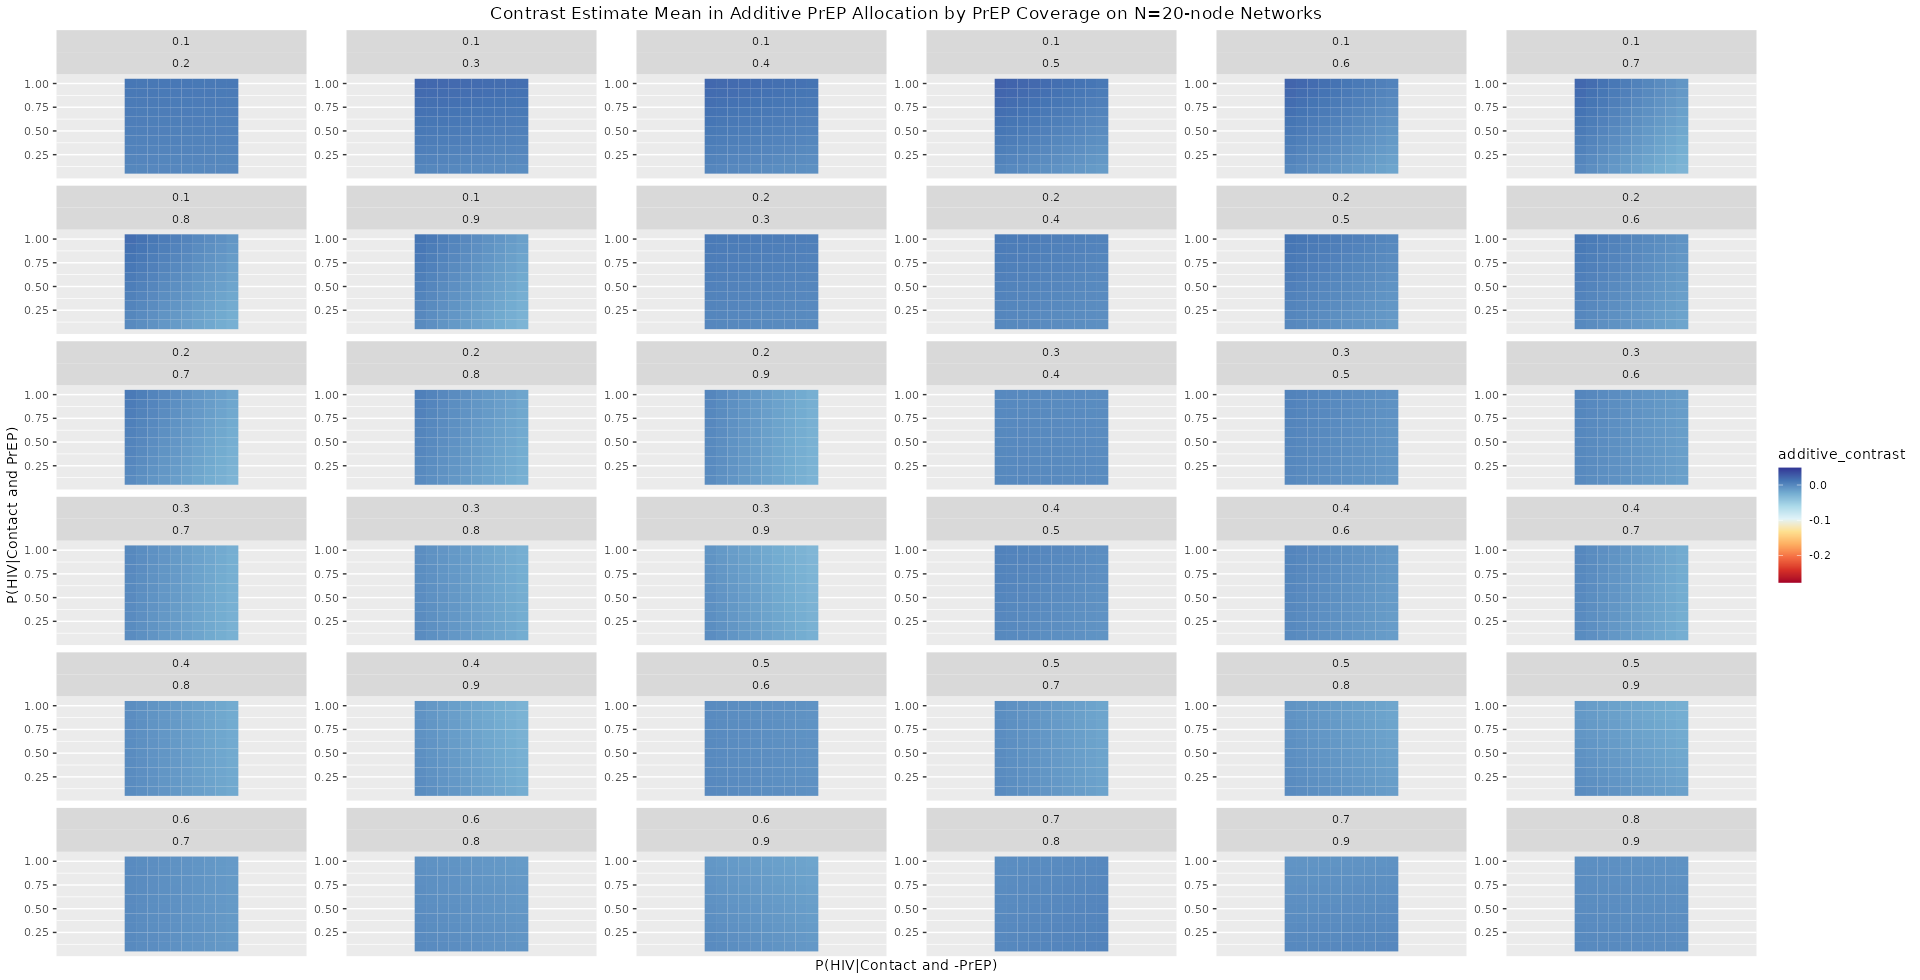
\includegraphics[width=\linewidth]{Corrected Figures/PrEP Additive Mean Plots.png}
    \caption{Mean Causal Contrast estimates as $\mathbb{P}\left[\text{HIV} \vert \neg \text{PrEP} \cap \text{Contact}\right]$ and $\mathbb{P}\left[\text{HIV} \vert \text{PrEP} \cap \text{Contact}\right]$ increase, stratified by random PrEP1\% additional vs. random PrEP2-PrEP1 \% PrEP allocation control. Top number indicates PrEP1 \% control coverage. Bottom number is PrEP2 counterfactual coverage. }
    \label{fig:Figure S4.11}
\end{figure}
\begin{figure}[H]
    \centering
    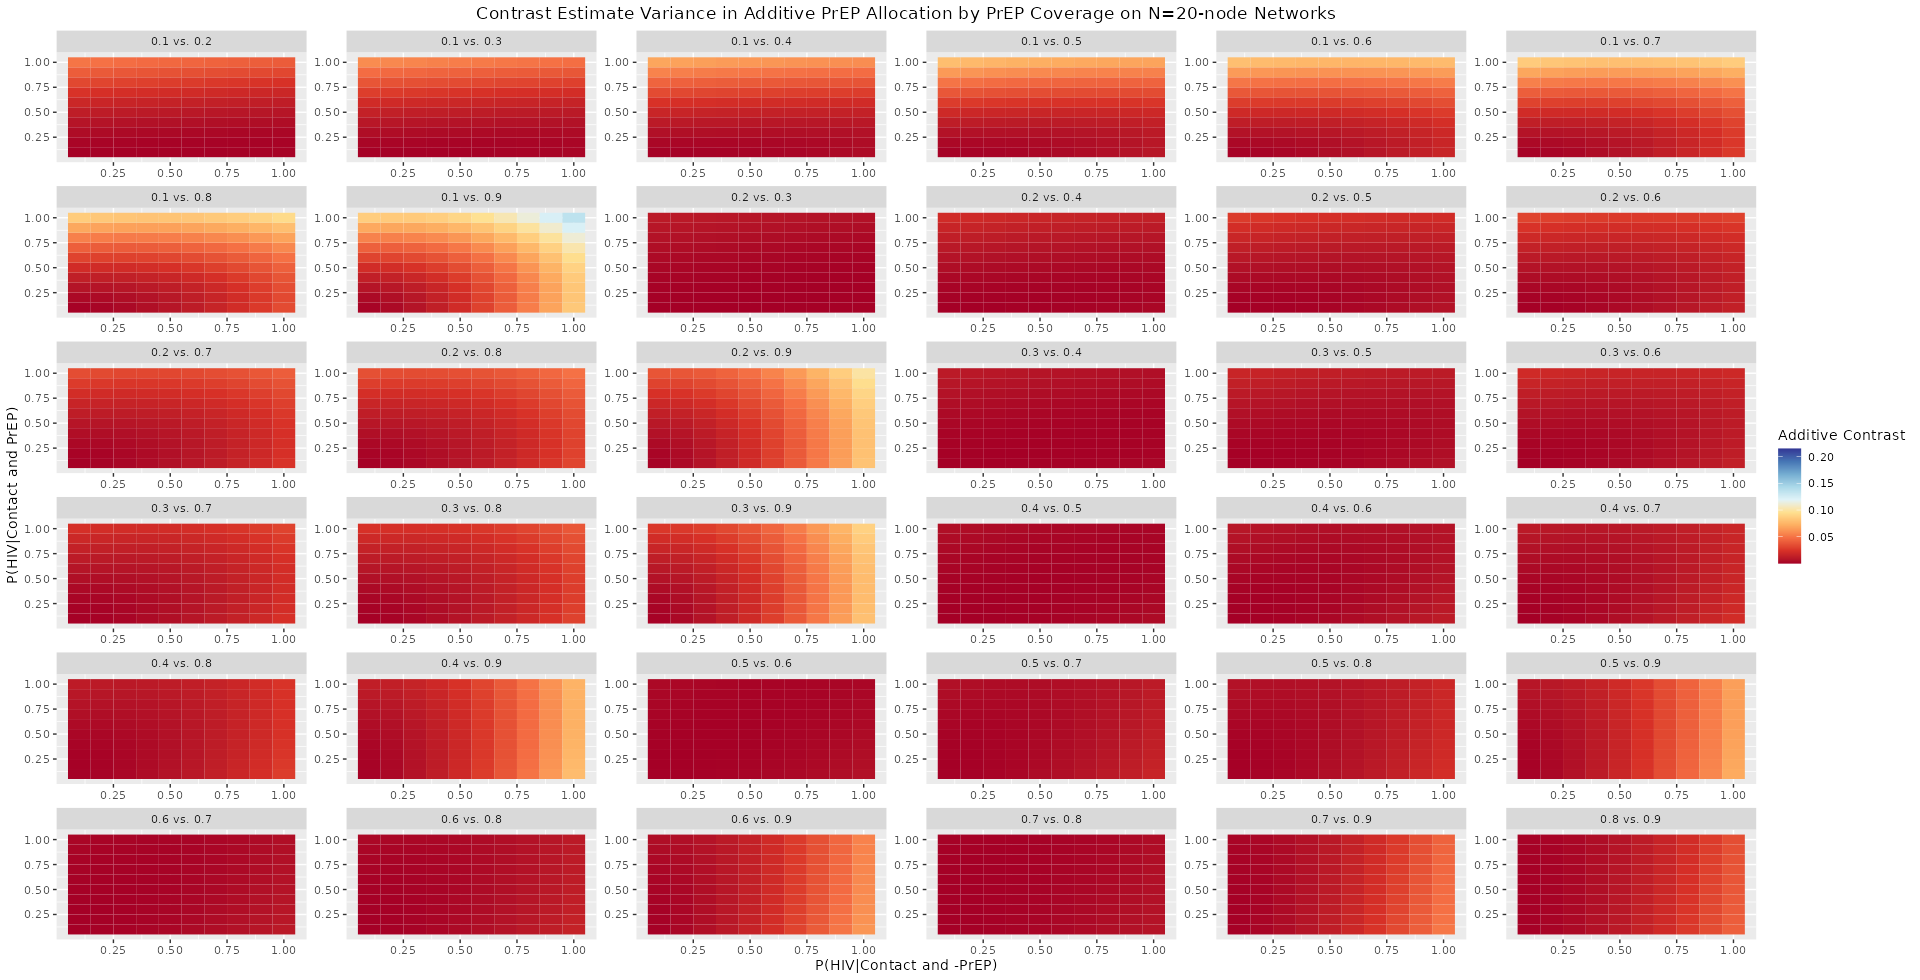
\includegraphics[width=\linewidth]{Corrected Figures/PrEP Additive Variance Plots.png}
    \caption{Variance of Causal Contrast estimates as $\mathbb{P}\left[\text{HIV} \vert \neg \text{PrEP} \cap \text{Contact}\right]$ and $\mathbb{P}\left[\text{HIV} \vert \text{PrEP} \cap \text{Contact}\right]$ increase, stratified by random PrEP2-PrEP1\% additional vs. random PrEP1 \% PrEP allocation control. Top number indicates PrEP1/control coverage. Bottom number is PrEP2 counterfactual coverage.}
    \label{fig:Figure S4.12}
\end{figure}
\begin{figure}[H]
    \centering
    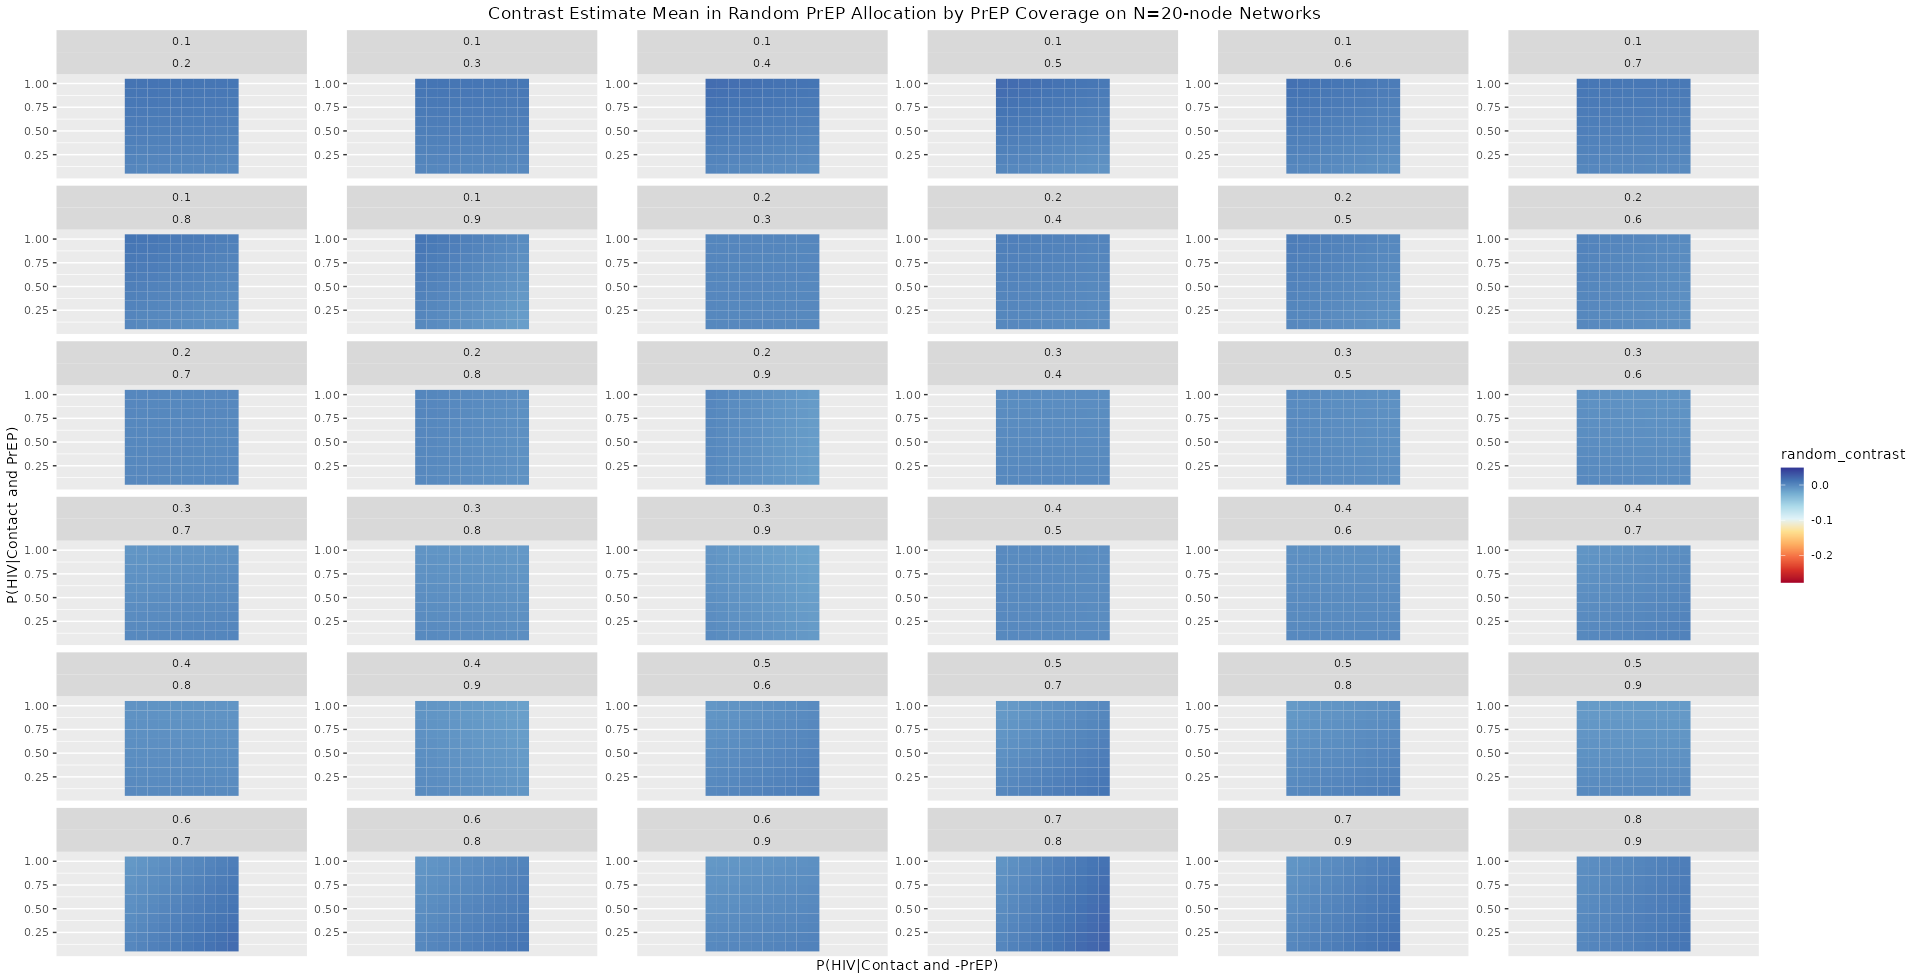
\includegraphics[width=\linewidth]{Corrected Figures/PrEP Random Mean Plots.png}
    \caption{Mean Causal Contrast estimates as $\mathbb{P}\left[\text{HIV} \vert \neg \text{PrEP} \cap \text{Contact}\right]$ and $\mathbb{P}\left[\text{HIV} \vert \text{PrEP} \cap \text{Contact}\right]$ increase, stratified by random PrEP2\% vs. random PrEP1\% PrEP allocation control. Top number indicates PrEP1/control coverage. Bottom number is PrEP2 counterfactual coverage.}
    \label{fig:Figure S4.13}
\end{figure}
\begin{figure}[H]
    \centering
    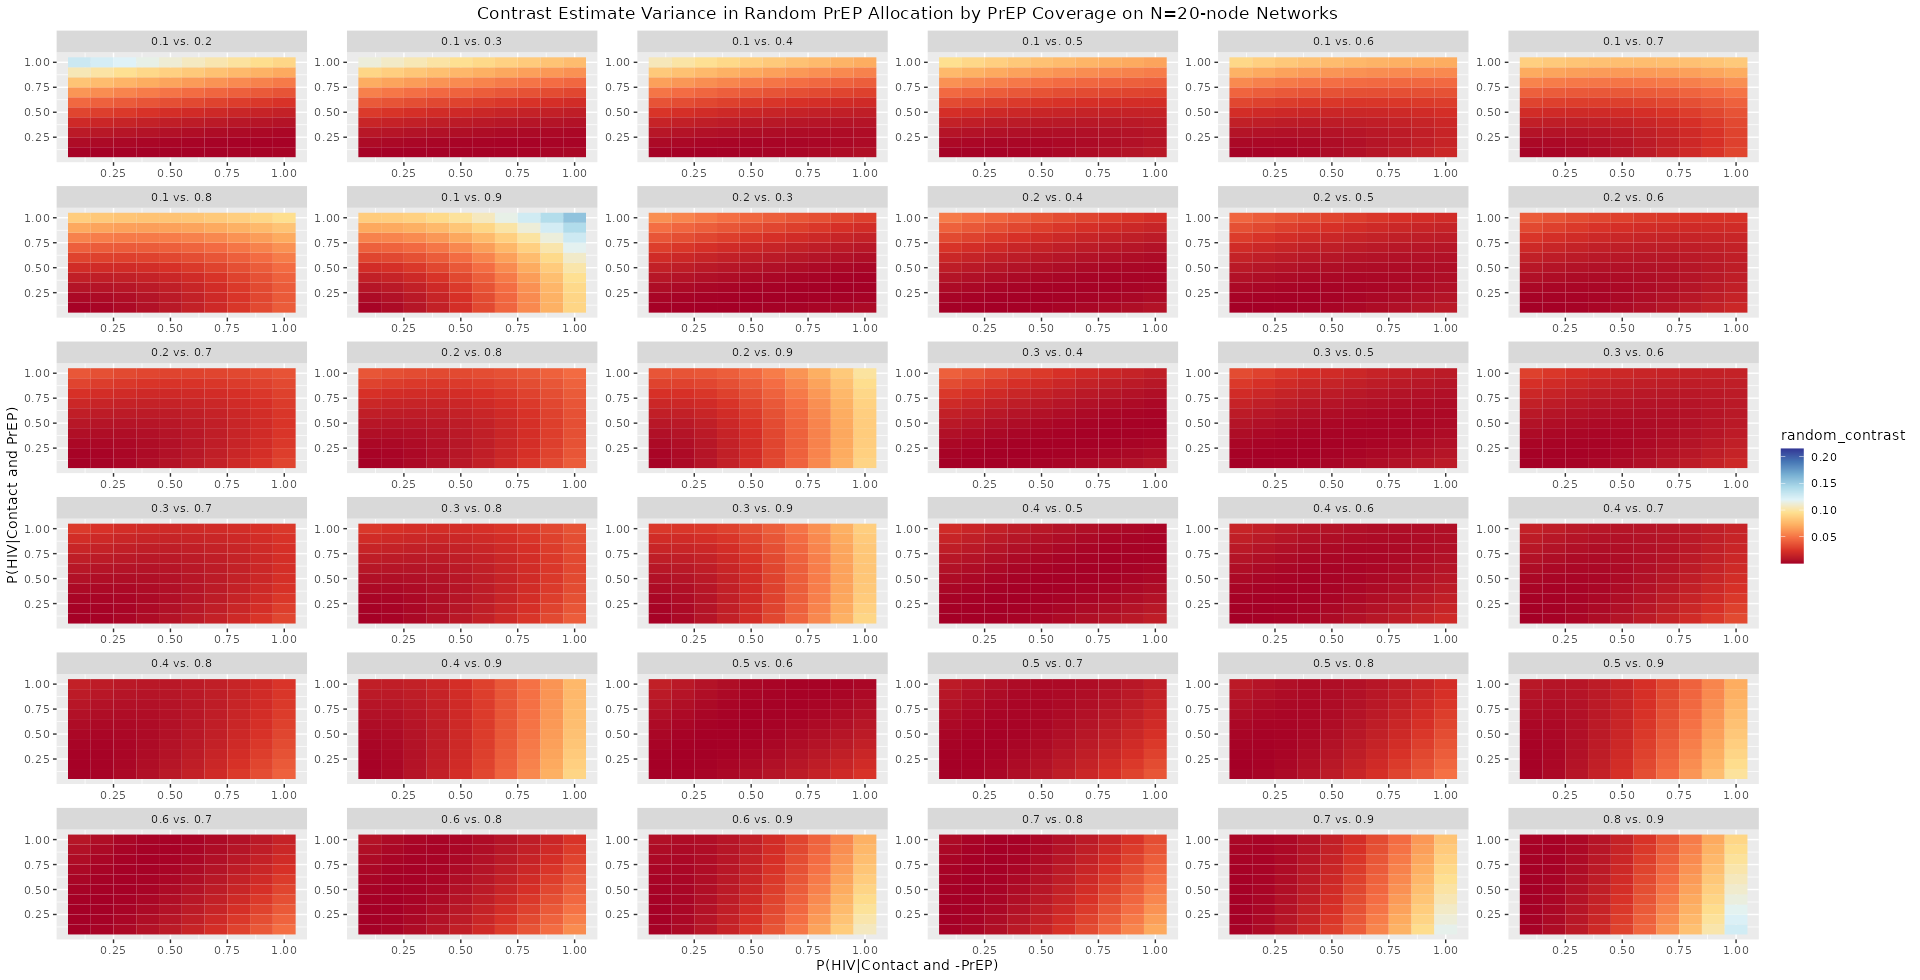
\includegraphics[width=\linewidth]{Corrected Figures/PrEP Random Variance Plots.png}
    \caption{Variance of Causal Contrast estimates as $\mathbb{P}\left[\text{HIV} \vert \neg \text{PrEP} \cap \text{Contact}\right]$ and $\mathbb{P}\left[\text{HIV} \vert \text{PrEP} \cap \text{Contact}\right]$ increase, stratified by random PrEP2\% vs. random PrEP1\% PrEP allocation control. Top number indicates PrEP1/control coverage. Bottom number is PrEP2 counterfactual coverage.}
    \label{fig:Figure S4.14}
\end{figure}
\begin{figure}[H]
    \centering
    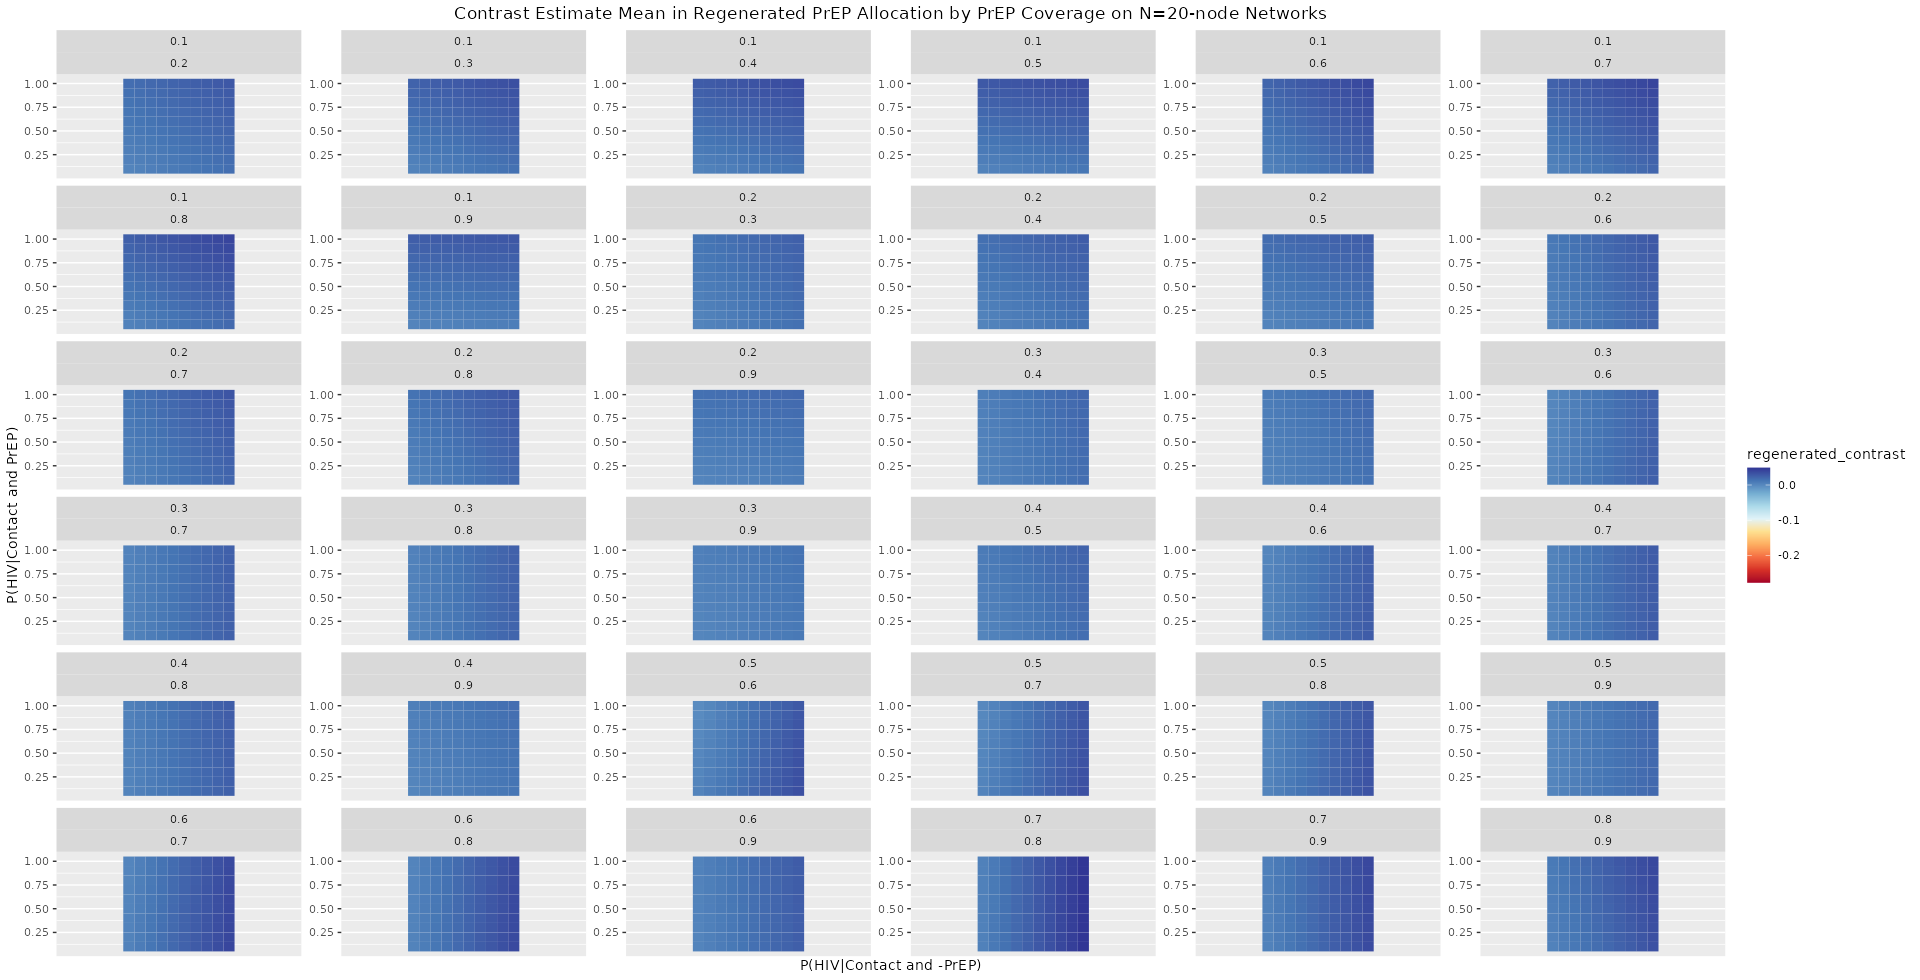
\includegraphics[width=\linewidth]{Corrected Figures/PrEP Regenerated Mean Plots.png}
    \caption{Mean of Causal Contrast estimates as $\mathbb{P}\left[\text{HIV} \vert \neg \text{PrEP} \cap \text{Contact}\right]$ and $\mathbb{P}\left[\text{HIV} \vert \text{PrEP} \cap \text{Contact}\right]$ increase, stratified by  random PrEP1 \% allocation vs random PrEP2\% allocation on a regenerated network. Top number indicates PrEP1/control coverage. Bottom number is PrEP2 counterfactual coverage.}
    \label{fig:Figure S4.15}
\end{figure}
\begin{figure}[H]
    \centering
    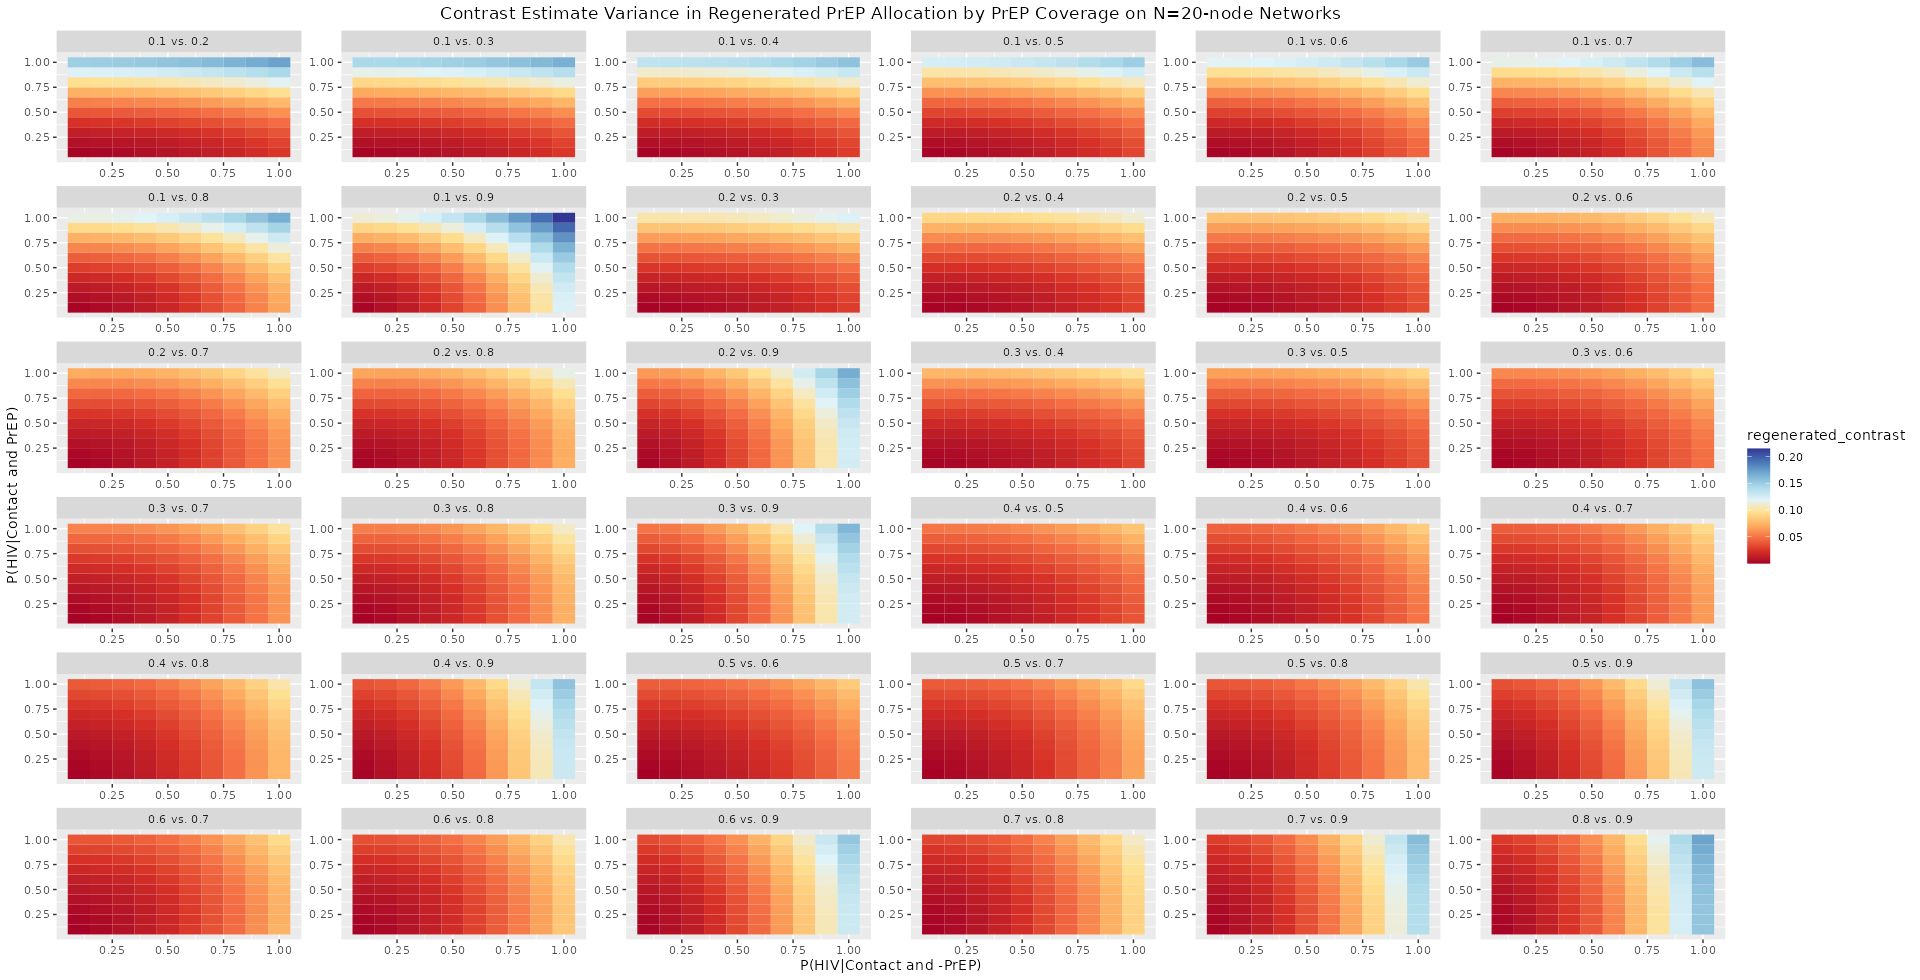
\includegraphics[width=\linewidth]{Corrected Figures/PrEP Regenerated Variance Plots.png}
    \caption{Variance of Causal Contrast estimates as $\mathbb{P}\left[\text{HIV} \vert \neg \text{PrEP} \cap \text{Contact}\right]$ and $\mathbb{P}\left[\text{HIV} \vert \text{PrEP} \cap \text{Contact}\right]$ increase, stratified by random PrEP1 \% allocation vs random PrEP2\% allocation on a regenerated network. Top number indicates PrEP1/control coverage. Bottom number is PrEP2 counterfactual coverage. }
    \label{fig:Figure S4.16}
\end{figure}

We can observe from the Causal Contrast Mean and Variance plots in Figures \ref{fig:Figure S4.11}-\ref{fig:Figure S4.16} that there is effect modification of the relationship between underlying HIV risks and treatment strategy by the choices of PrEP treatment contrasts. This modification is easier to identify in the Variance plots, as once again the variances for the regenerated allocation strategy contrasts display a completely different gradient across underlying risks from the additive and random strategy for all pairs of PrEP coverages. While the gradients are more similar between the random and additive strategies, there are still clear differences in contrast Variance magnitude for given choices of PrEP coverage and HIV risks. With respect to the contrast estimate Mean, effect modification is more subtle between the random and additive strategies and more apparent when comparing these two to the regenerated strategy contrasts. 
\subsection{Other Network Models}

\subsubsection{Effect Modification by Network Generating Model with Default Parameters}
\begin{figure}[H]
    \centering
    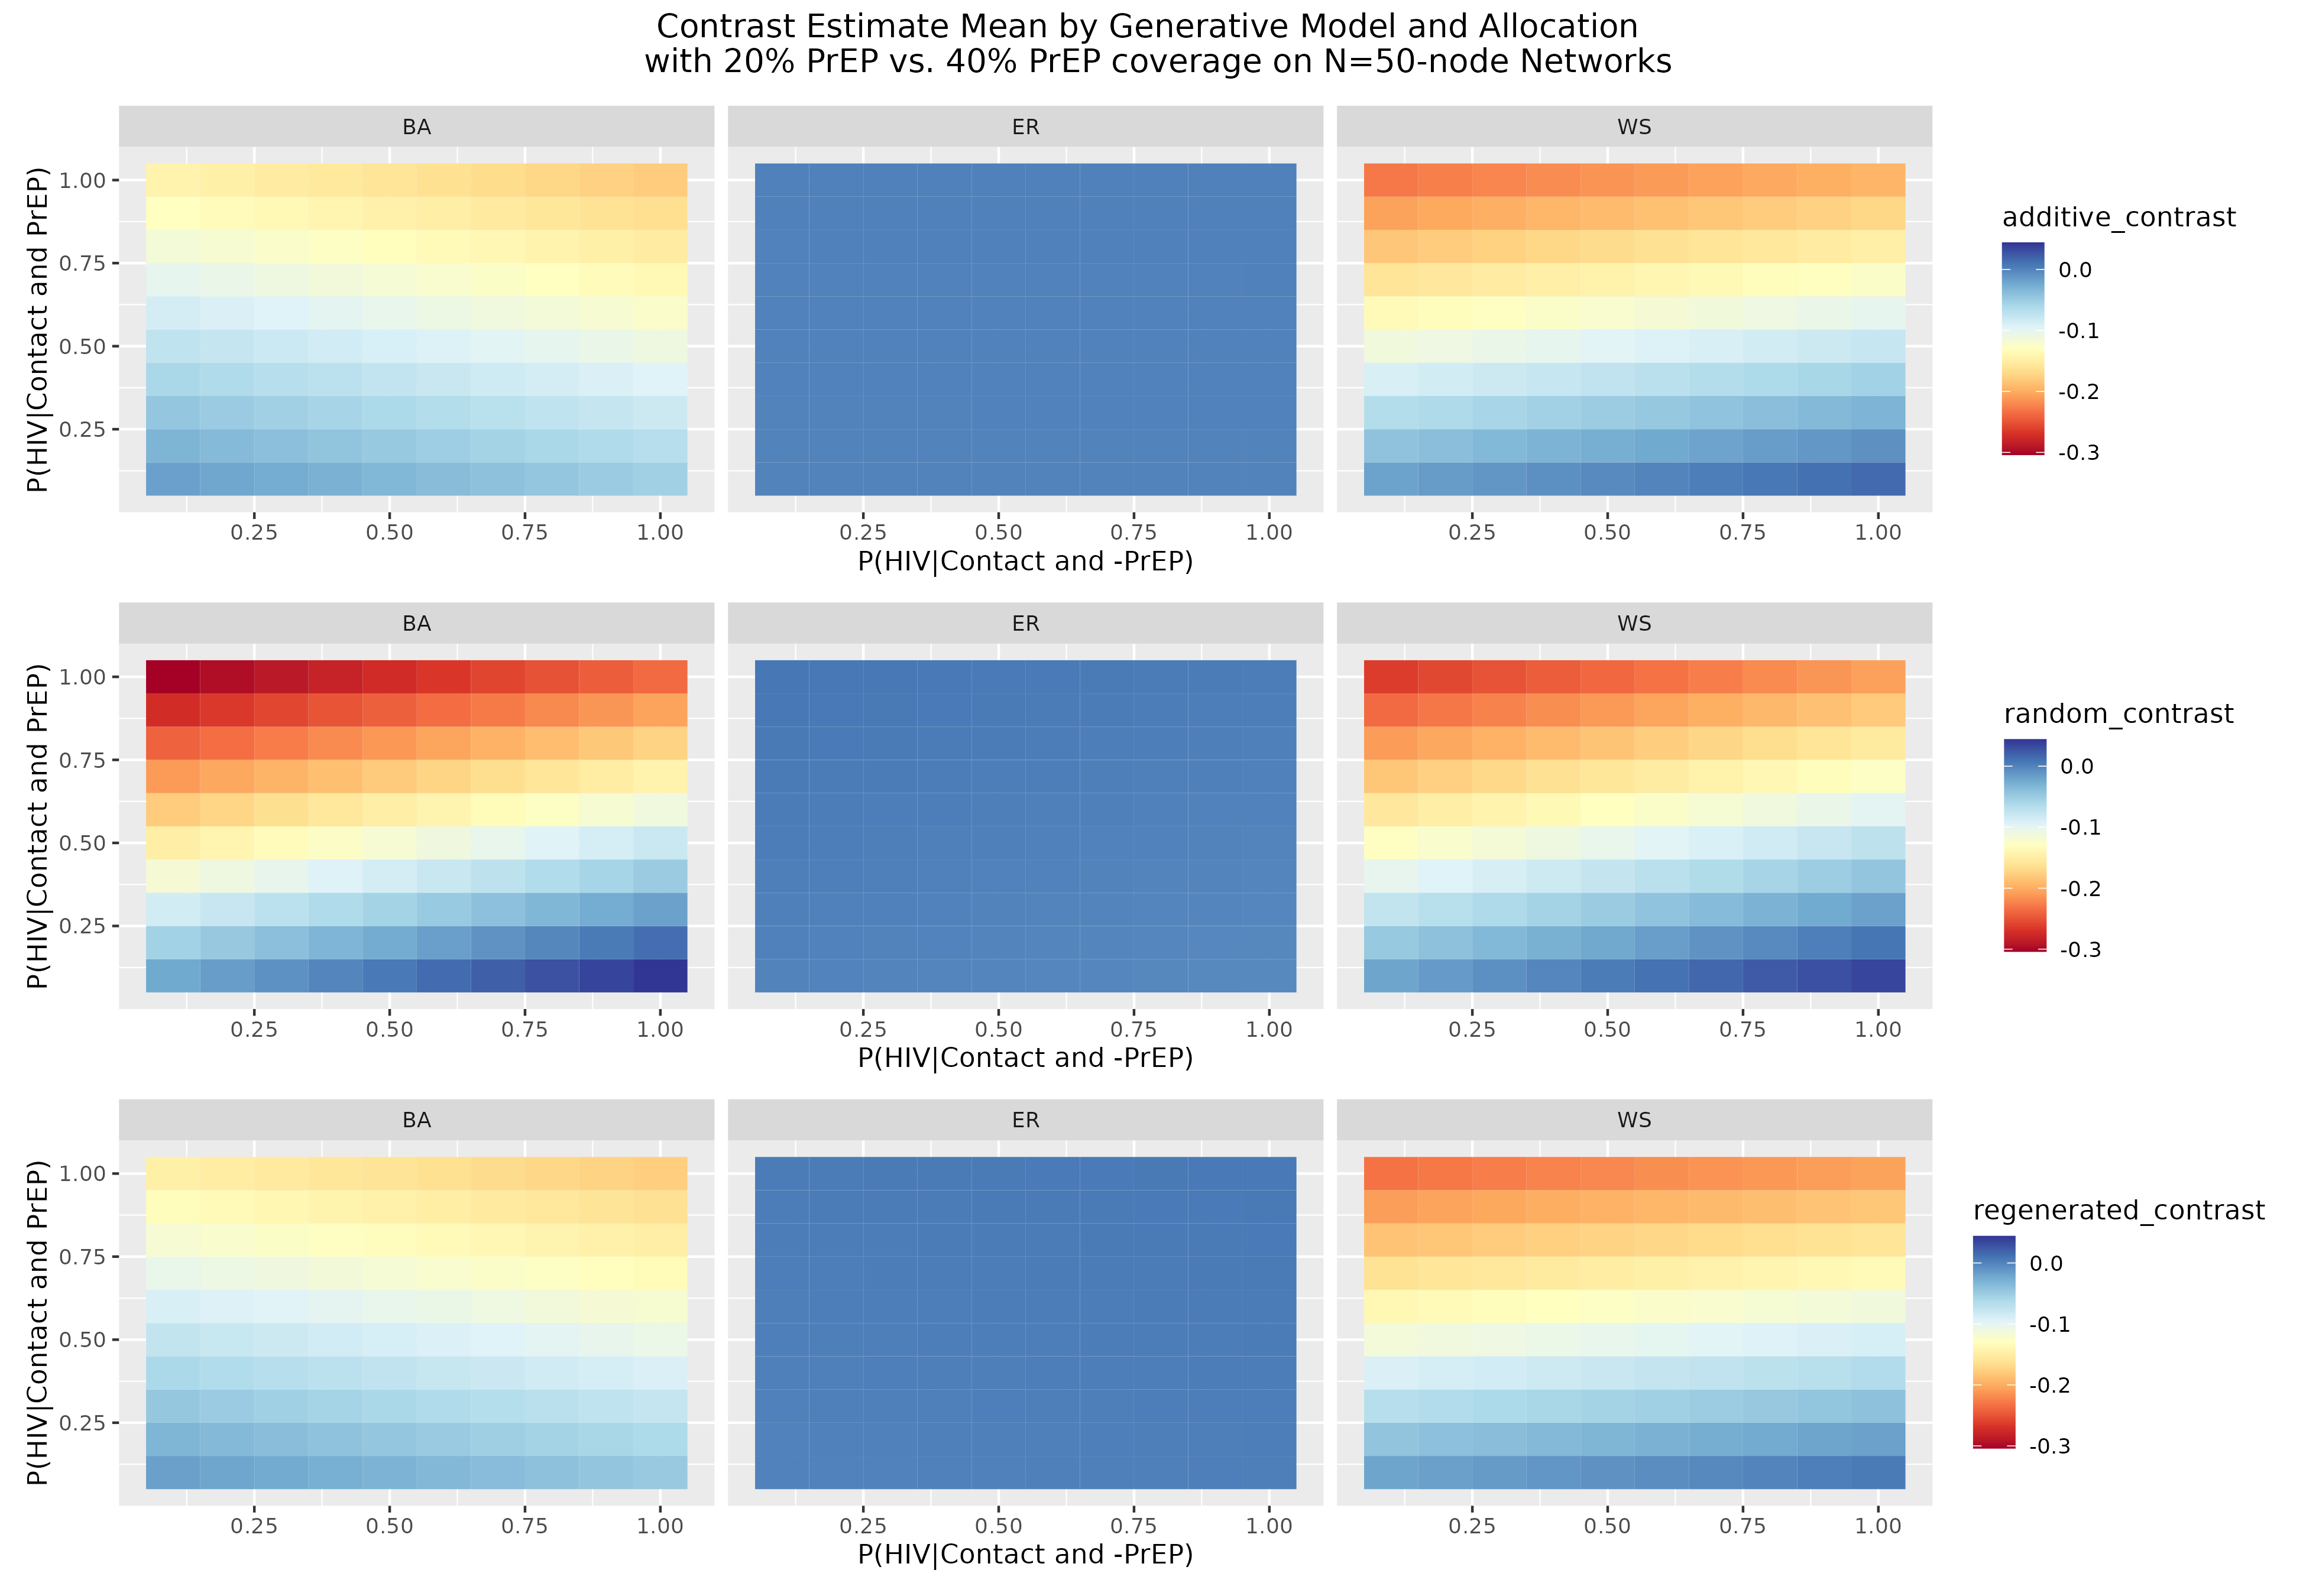
\includegraphics[width=\linewidth]{Corrected Figures/Generative Model Mean Plot.png}
    \caption{Mean of Causal Contrast estimates as $\mathbb{P}\left[\text{HIV} \vert \neg \text{PrEP} \cap \text{Contact}\right]$ and $\mathbb{P}\left[\text{HIV} \vert \text{PrEP} \cap \text{Contact}\right]$ increase, stratified by the model used to generate the networks, and by estimator. From left to right, ``BA" the Barabási–Albert scale-free model, ``ER" the Erdős–Rényi Random Graph model, ``WS" the Watts-Strogatz Small-World model. From top to bottom: ``additive" Mean Contrast of random 20\% additional vs. random 20\% PrEP allocation control, ``random" Mean Contrast of random 40\% PrEP allocation vs. random 20\% control, ``regenerated" Mean Contrast of random 40\% allocation on regenerated network vs. random 20\% control. }
    \label{fig:Figure S4.17}
\end{figure}
From the Causal Contrast Mean plots in Figure \ref{fig:Figure S4.17} above, we can see stark effect modification of the relationship between underlying HIV risks and treatment strategy by the choice of network generative model. In particular, the ER model displays a completely different gradient than those of the BA or WS models for all treatment strategies. There is also a ``reversal" in the direction of effects for the BA model with random allocation compared to additive and regenerated strategies, as well as relatively large differences in magnitude of effect estimates. WS model effect estimate magnitudes are also different across treatment strategies. 

\begin{figure}[H]
    \centering
    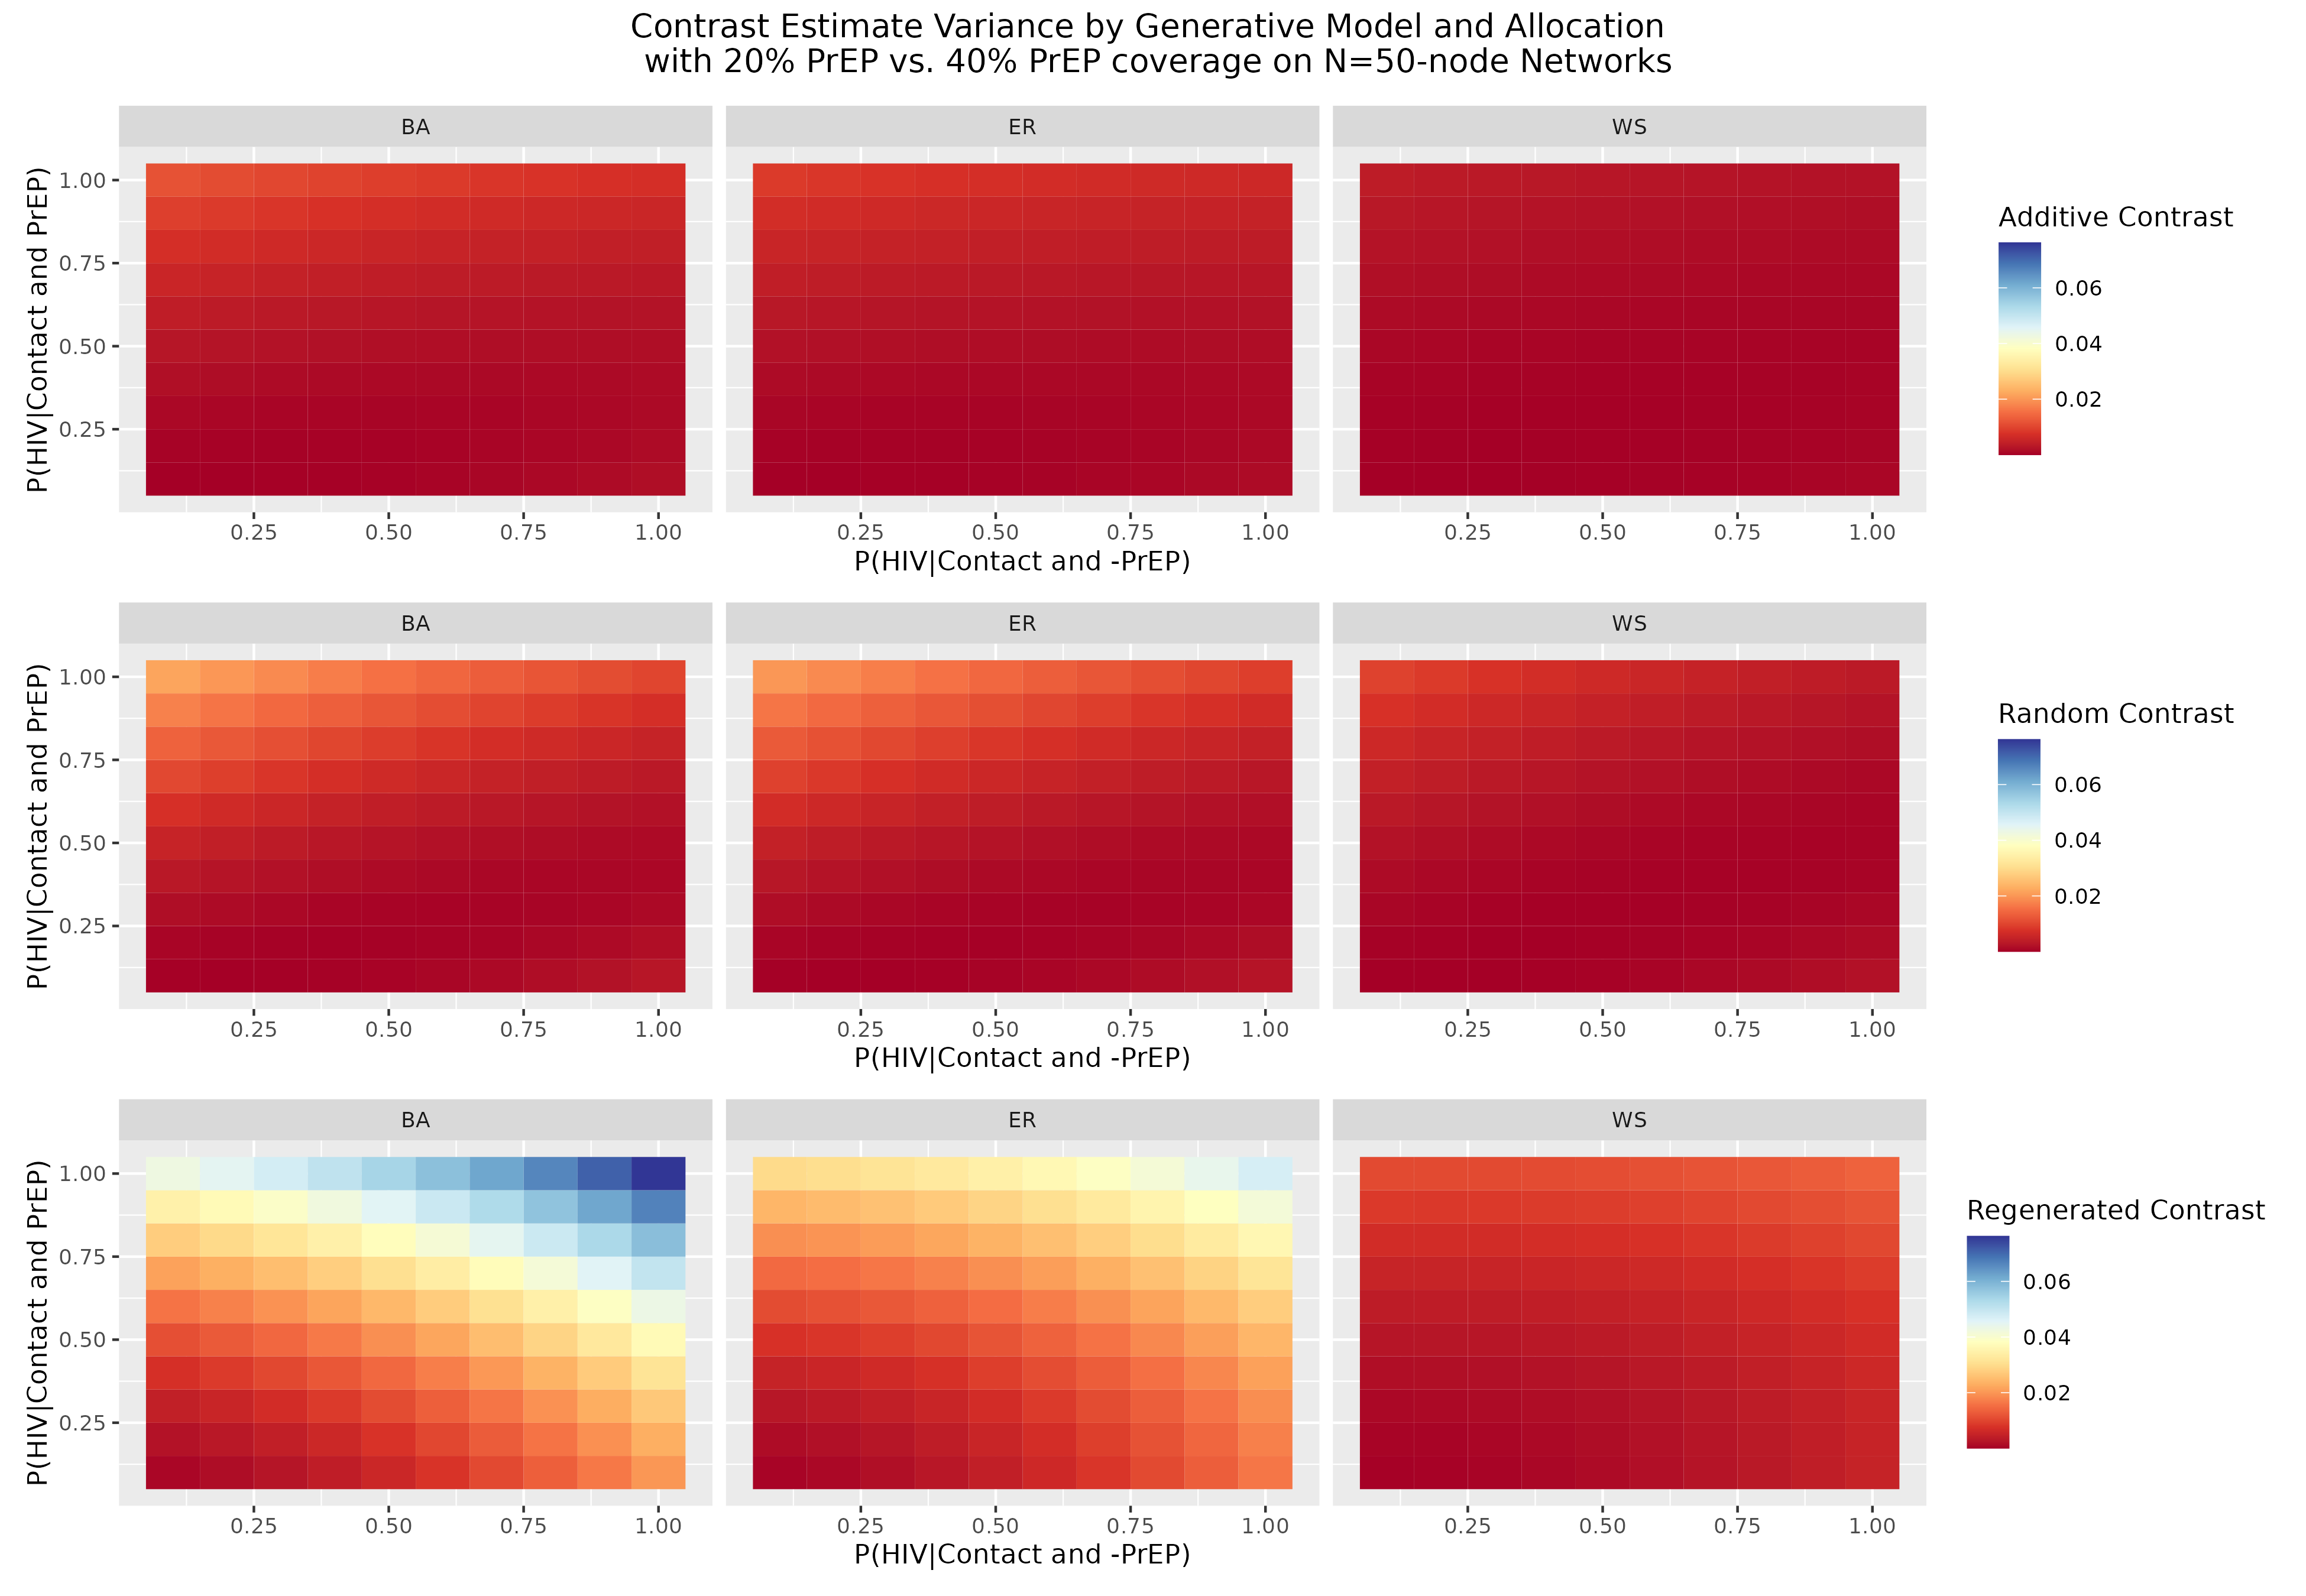
\includegraphics[width=\linewidth]{Corrected Figures/Generative Model Variance Plot.png}
    \caption{Variance of Causal Contrast estimates as $\mathbb{P}\left[\text{HIV} \vert \neg \text{PrEP} \cap \text{Contact}\right]$ and $\mathbb{P}\left[\text{HIV} \vert \text{PrEP} \cap \text{Contact}\right]$ increase, stratified by stratified by the model used to generate the networks, and by estimator. From left to right, ``BA" the Barabási–Albert scale-free model, ``ER" the Erdős–Rényi Random Graph model, ``WS" the Watts-Strogatz Small-World model. From top to bottom: ``additive" Variance of Contrast of random 20\% additional vs. random 20\% PrEP allocation control, ``random" Variance of Contrast of random 40\% PrEP allocation vs. random 20\% control, ``regenerated" Variance of Contrast of random 40\% allocation on regenerated network vs. random 20\% control.}
    \label{fig:Figure S4.18}
\end{figure}
The Causal Contrast Variance plots in Figure \ref{fig:Figure S4.18} above also clearly show effect modification  of the relationship between underlying HIV risks and treatment strategy by the choice of network generative model.  Interestingly, the Variance gradients appear similar across models in the ``additive" allocation strategy. While the magnitudes of Variance estimates vary slightly, the gradient for the Watts-Strogatz model is much more consistent  across allocation strategies than for the Barabási–Albert or  Erdős–Rényi models. In particular, the gradients within these two models are markedly different by allocation strategy, although the pattern of changes is similar between these models across strategies. 


\end{document}